\status{review}
\chapter{muEDM}
\label{ch:muEDM}
\begin{refsection}

{\itshape
This chapter is an introduction to the muEDM experiment. After describing in some detail the spin dynamics, a reminder on the EDM searches for the different particles will follow.
We will then outline the measuring principle of the experiment, the frozen spin technique, and a deep dive into the current status of the experiment. 
The study of systematic uncertainties and the upcoming schedule will close this chapter. 
As always, the early stage of the experiment means the rate of changes and improvement is outstanding. 
This is my attempt at an up-to-date description, which relies on the ``muEDM Status Report 2023'' submitted to PSI, but some details might be already outdated.}

\cite{muEDM:Semertzidis:2001} \cite{muEDM:Adelmann:2010} \cite{muEDM:J-PARC:2011} \cite{muEDM:J-PARC:2016} \cite{muEDM:PSI:2021} \cite{muEDM:PSI:Mikio:2022} \cite{muEDM:PSI:Kim:2022}

\status{review}
\section{Electric Dipole Moment}
    As introduced in \ref{intro:edm}, the Hamiltonian describing the spin dynamics is:
    \begin{equation*}
        \hat{H} = -\mu\bm{\hat{\sigma}\cdot B}-d\bm{\hat{\sigma}\cdot E}
    \end{equation*}
    We then saw that, when considering a combination of magnetic and electric fields and a moving particle it is useful to introduce the polarization vector $\bm{\Pi}=\bm{s}/s$ and the Thomas precession $\bm{\Omega}_0$:
    \begin{equation*}
        \dv{\bm{\Pi}}{t}=\bm{\Omega}_0 \times \bm{\Pi}, \quad
        \bm{\Omega}_0 = -\frac{e}{m\gamma} \left[ (1+\gamma a)\bm{B}-\frac{a\gamma^2}{\gamma+1}(\bm{\beta}\cdot\bm{B})\bm{\beta}-\gamma \left( a+\frac{1}{\gamma+1} \right) \frac{\bm{\beta}\times \bm{E}}{c} \right]
    \end{equation*}
    With no electrical field parallel to the momentum and with $\bm{\Omega}_c$ the cyclotron frequency, the relative spin precession of a muon in a storage ring is described by (T-BMT \cite{miss-59}):
    \begin{equation}
        \begin{split}
            \bm{\Omega}=\bm{\Omega}_0-\bm{\Omega}_c &=
            \underbrace{ 
                \frac{q}{m}\left[ a\bm{B} -{\frac{a\gamma}{\gamma+1}(\bm{\beta}\cdot \bm{B})\bm{\beta}} - \left(  a+\frac{1}{1-\gamma^2}\right)\frac{\bm{\beta} \times \bm{E}}{c} \right]
            }_{\text{Anomalous precession, } \omega_a=\omega_L-\omega_c} \\&+
            \underbrace{
                \frac{\eta q}{2m}\left[ \bm{\beta} \times \bm{B} + \frac{\bm{E}}{c}- {\frac{\gamma c}{\gamma+1}(\bm{\beta}\cdot\bm{E\beta})} \right]
            }_{\text{Interaction of EDM and relativistic $\bm{E}$, } \omega_a}
        \end{split}
        \label{eq:muedm:precession}
    \end{equation}
    The second term describes the precession due to the \gls{edm} coupling to the relativistic $\bm{E}$, perpendicular to the $\bm{B}$ in which the particle is moving. 
    In the presence of a muon \gls{edm} the plane would be tilted and a vertical precession ($\bm{\omega}_e\perp\bm{B}$), shifted by $\pi/2$ to the horizontal anomalous precession, would become observable.

    \status{review}
    \subsection{Symmetry violation}
        In physics, there are three cardinal discrete symmetries: Charge (C), Parity (P), and Time (T).
        P and T are related to the invariance under spatial and temporal reversal while C is the invariance for particle $\leftrightarrow$ \textit{anti}particle exchange.
        While the magnetic field and the spin are \textit{pseudo}-vectors under P and vectors under T, the electric field behaves in the opposite way.
        The implication of this difference is that EDM and MDM behave differently under C, P, and T:
        \begin{equation}
            MDM : 
            \begin{cases}
                \textbf{P} (-\mu\bm{\hat{\sigma}\cdot B}) = -\mu \bm{P(\hat{\sigma}) \cdot P(B)} = -\mu\bm{(+\hat{\sigma})\cdot (+B)} = -\mu\bm{\hat{\sigma}\cdot B} \\
                \textbf{T} (-\mu\bm{\hat{\sigma}\cdot B}) = -\mu \bm{T(\hat{\sigma}) \cdot T(B)} = -\mu\bm{(-\hat{\sigma})\cdot (-B)} = -\mu\bm{\hat{\sigma}\cdot B} 
            \end{cases}
        \end{equation}
        \begin{equation}
            EDM : 
            \begin{cases}
                \textbf{P} (-d\bm{\hat{\sigma}\cdot E}) = -d \bm{P(\hat{\sigma}) \cdot P(E)} = -d\bm{(+\hat{\sigma})\cdot (-E)} = +d\bm{\hat{\sigma}\cdot E} \\
                \textbf{T} (-d\bm{\hat{\sigma}\cdot E}) = -d \bm{T(\hat{\sigma}) \cdot T(E)} = -d\bm{(-\hat{\sigma})\cdot (+E)} = +d\bm{\hat{\sigma}\cdot E}          
            \end{cases}
        \end{equation}
        In light of the CPT theorem, the breaking of the T symmetry implies the breaking of CP.
        
    \status{review}
    \subsection{Current limits on EDM}
        As discussed in \ref{sec:exp:edm}, the last decades saw a continuous effort to measure the EDM of different particles.
        There the experiments setting the current limits were discussed but we report in Tab.~\ref{tab:edm} the results to aid the reader.
        It is important to note there are two limits for $\upmu$: one obtained by rescaling the limit on $d_e$, obtaining an \textit{indirect limit}; one, less stringent, is a \textit{direct} limit ($^*$).
        
        \setcounter{table}{0}
        \begin{table}[h]
            \centering
            \begin{tabular}{|c|c|c|}
                \hline
                Experiment & Particle & EDM limit in ecm \\
                \hline
                \hline
                nEDM \cite{nEDM} & n & \num{0.18e-25}\\
                \hline
                ACME \cite{eEDM:ACME} & e & \num{1.1e-29} \\
                \hline
                Indirect \cite{muEDM:indirect} & $\upmu$ & \num{0.19e-19} $^*$ \\
                \hline
                g-2 \cite{muEDM:direct} & $\upmu$ & \num{1.8e-19} \\
                \hline
            \end{tabular}
            \caption[]{Sumary of the current limits on the EDM for neutron electron and muon.}
            \label{tab:edm}
        \end{table}

    \status{review}
    \subsection{The \textit{frozen spin} technique}
        
        As illustrated in \cite{1,9}, with the appropriate choice of electric field and having $\bm{p}$, $\bm{B}$ and $\bm{E}$ forming an orthogonal basis, the anomalous precession term in eq. \ref{eq:muedm:precession} can be set to zero. 
        \begin{equation}
            a\bm{B}=\left( a-\frac{1}{\gamma^2-1} \right)\frac{\bm{\beta}\times\bm{E}}{c}
        \end{equation}
        In this situation the relative angle between $\bm{p}$ and spin remains unchanged if $\eta=0$, hence 'frozen'. 
        In the presence of an \gls{edm} the change in polarization would then follow
        \begin{equation}
            \label{eq:freezed}
            \dv{\bm{\Pi}}{t}=\bm{\omega}_e \times \bm{\Pi}, \quad
            \bm{\omega}_e=\frac{\eta q}{2m} \left(\bm{\beta}\times\bm{B}+\frac{\bm{E}_f}{c} \right) =
            \frac{2 d_\mu}{\hbar} \left(\bm{\beta}c\times\bm{B}+\bm{E}_f\right)
        \end{equation}
        The net result of the \gls{edm} is then a vertical build-up of the polarization given by Eq.~\ref{eq:edm:polarization} and illustrated by the sketch in Fig.~\ref{fig:muEDM:g-2_EDM}.
        \begin{equation}
            |\bm{\Pi}(t)|=P(t)=P_0\sin(\omega_e t)\approx P_0 \omega_e t \approx 2P_0\frac{d_\mu}{\hbar}\frac{E_f}{a\gamma^2}t
            \label{eq:edm:polarization}
        \end{equation}    
        The evaluation of the sensitivity will follow a brief introduction to the muEDM experiment, to better familiarize the reader with the system.

        \begin{figure}
            \centering
            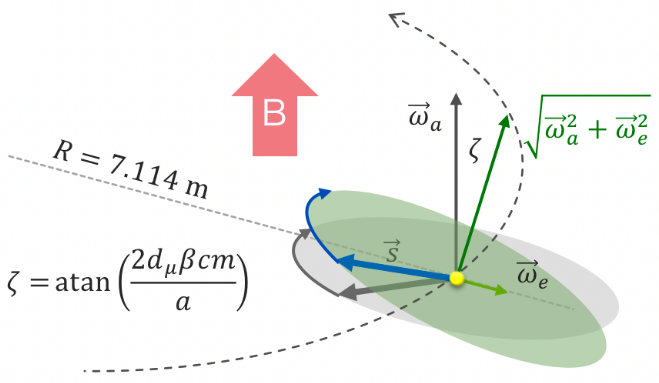
\includegraphics[width = 0.6\textwidth]{Figures/muEDM/g-2_EDM.png}
            \caption{}
            \label{fig:muEDM:g-2_EDM}
        \end{figure}

\status{review}
\section{The muEDM experiment}
    In the upcoming years, we plan to search for a muon Electric Dipole Moment (EDM) using an existing solenoid, as shown in Fig.~\ref{fig:PSCSolenoid}. 
    The experiment will be connected to a surface muon beam line at PSI, delivering approximately \SI{4e6}{\upmu \per s} of $p=\SI{28}{MeV/c}$. 
    The muons are confined in a transverse phase space of $\epsilon_{xx'}= 192\ \pi$mmrad and $\epsilon_{yy'}= 171\ \pi$mmrad. 
    To enhance precision, a long copper tube within a superconducting shield is employed for collimation, reducing the number of muons inside the solenoid to about \SI{1.2e5}{\upmu \per s}. 
    A precisely timed magnetic pulse is then used to capture and store the selected muons within the weakly focusing magnetic field.
    
    A trigger is generated from the anticoincidence between two scintillators at the collimation channel exit. 
    This setup allows us to store only one muon at a time, with an expected rate of about \SI{800}{\upmu \per s} meeting the required conditions. 
    During storage, muons circulate with a radius of $r=\SI{31}{mm}$, and a scintillating fiber tracker is employed to track the direction of the positron resulting from muon decay. 
    The precession frequency, $\Omega$, is extracted by measuring the oscillation of the positron energy distribution as a function of decay time. 
    The frozen-spin condition is determined when $\Omega(E)=0$, allowing for the measurement of a non-zero EDM.
    
    In the presence of an EDM, the muon spin precesses out of the orbit plane, influencing the decay positron's trajectory. 
    By detecting the decay asymmetry, we can identify the EDM. 
    The project is to divide the task in to phases.
    During Phase I, the highest sensitivity is achieved for positron momenta above \SI{40}{MeV/c}, resulting in a mean asymmetry of about $A=0.35$.
    With an expected sensitivity of $\sigma(d_\mu)<\SI{2.8E-16}{ecm}$ per muon, we anticipate achieving $\sigma(d_\mu)<\SI{3E-21}{ecm}$ in a year of data taking with a detection rate of $N=\SI{300}{\per\second}$ positrons.
    
    \begin{figure}%
    \centering
        \subfloat[Picture of the muEDM superconducting solenoid.]{
        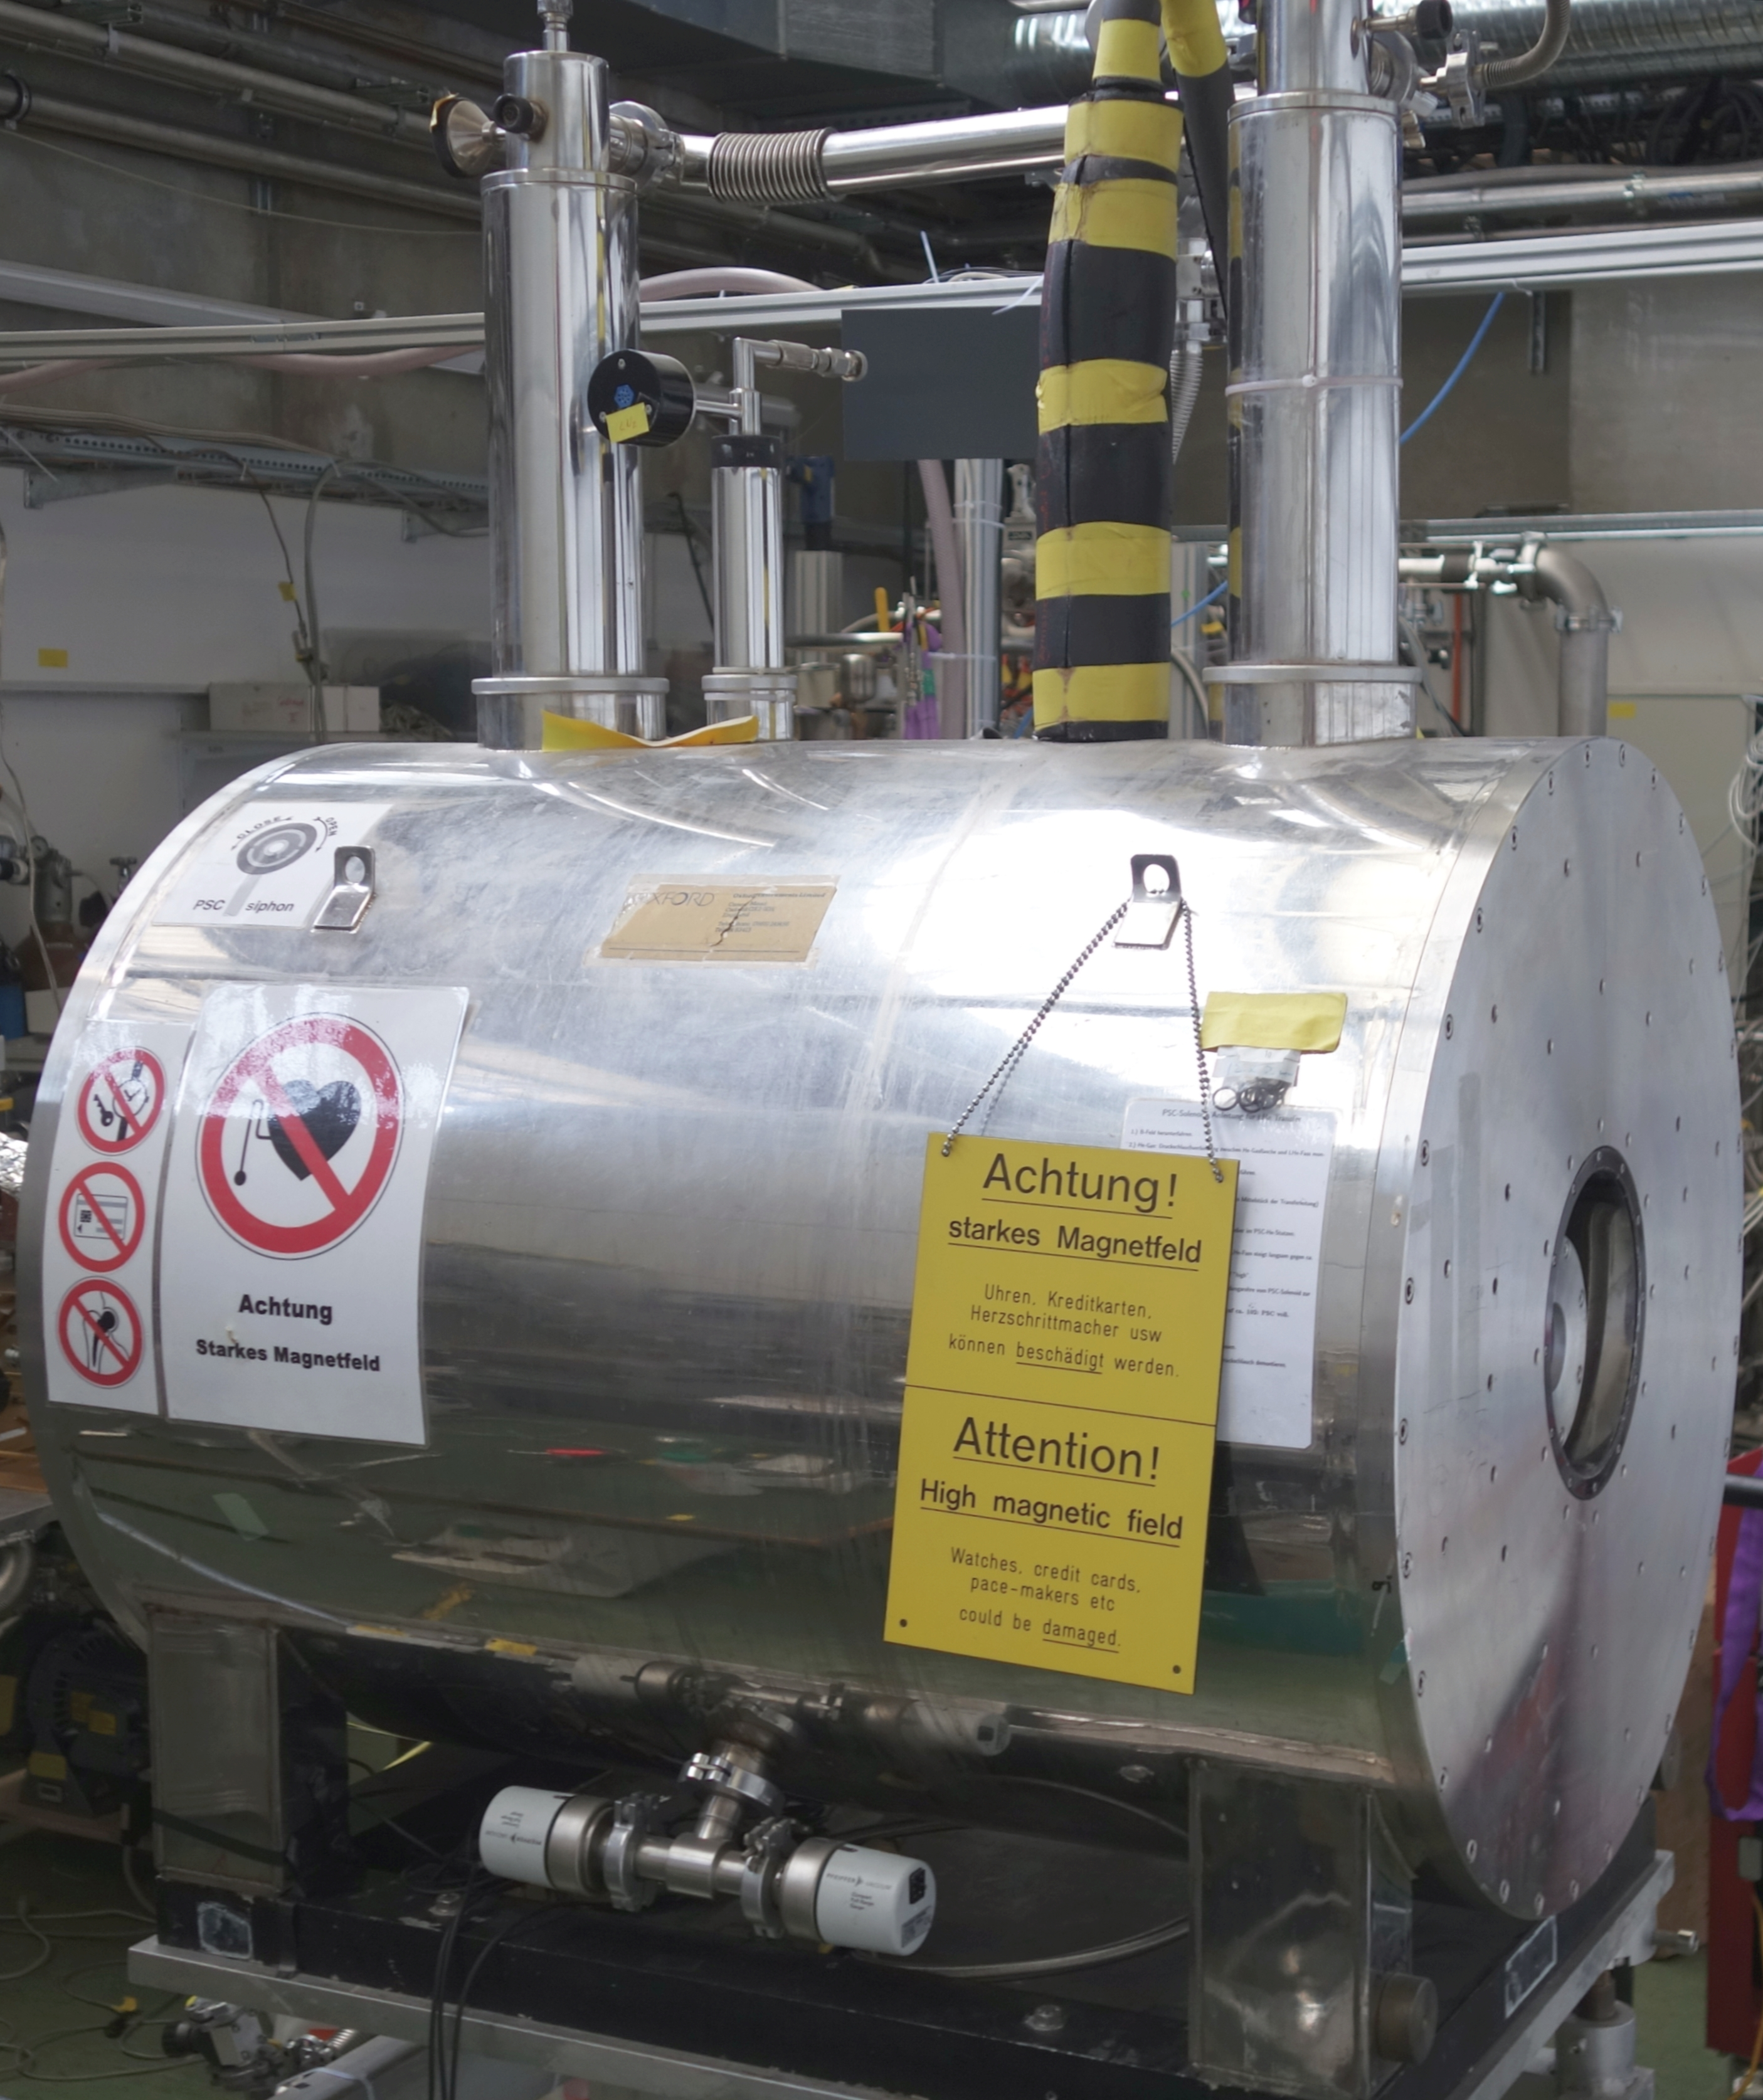
\includegraphics[width=0.35\columnwidth]{Figures/muEDM/PSCSolenoid.jpg}
        \label{fig:PSCSolenoid}}%
        \hfill
        \subfloat[Sketh of the muEDM setup.]{
        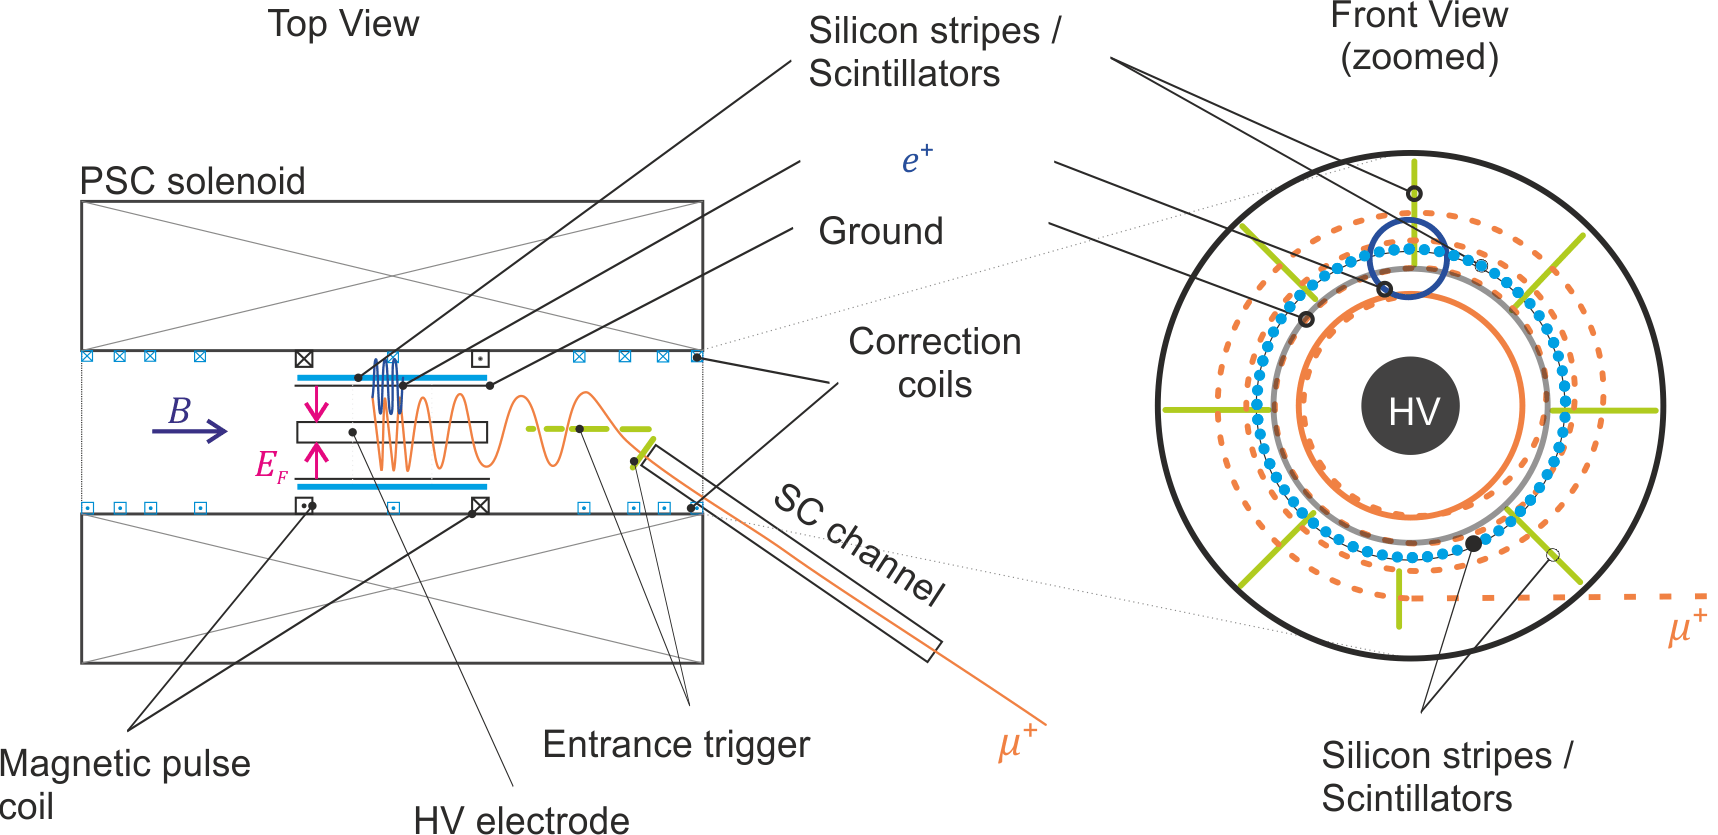
\includegraphics[width=0.60\columnwidth]{Figures/muEDM/PSC-FrozenSpin2023.png}
        \label{fig:PrecusorSketch}}
        \caption{Photo~(a) and sketch~(b) of the compact superconducting solenoid and the experimental setup for the search for the EDM of the muon. The warm bore of the solenoid has an inner diameter of \SI{200}{mm} and an outer diameter of about \SI{1000}{mm}.}%
    \label{fig:PhaseISetup}%
    \end{figure}

\begin{figure}
\centering
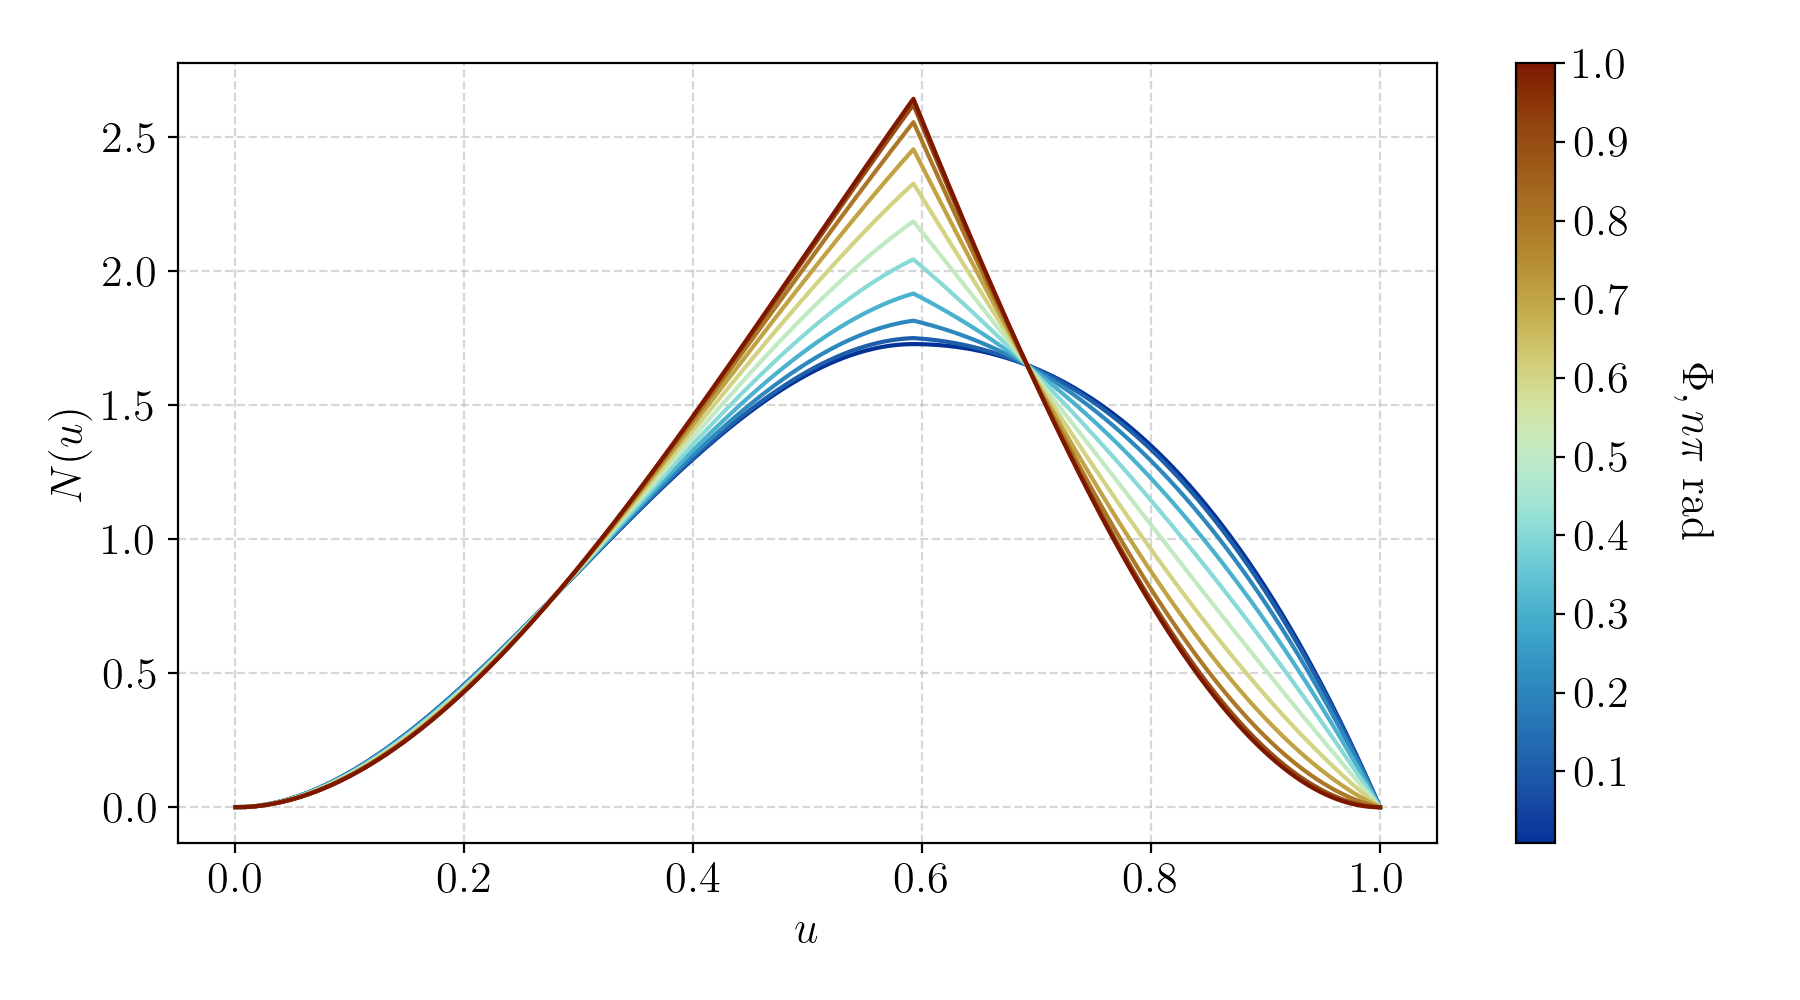
\includegraphics[width=0.66\columnwidth]{Figures/muEDM/n_vs_phi.png}
\caption{Positron energy distribution as a function of the angle between the muon spin and momentum. The fractional energy $u = E/E_\text{max}$ is shown on the abscissa. The maximum positron energy for Phase~I is $E_\text{max} = \SI{68.9}{MeV}$. The color bar shows the $g-2$ phase in units of $\pi$ radians, where 0 is spin and momentum aligned (blue) and 1 is anti-aligned (red).
}%
\label{fig:n_vs_phi}
\end{figure}

\status{review}
\section{The precursor}
    The task at hand is quite complex and for this reason, the aim is to first have a working prototype to demonstrate the measuring principles, the achieved control on the different sources of uncertainties, and the correct working of the different subdetectors.
    A review of the design and status of the different parts will be now given, in order of appearance during an event:
    \begin{center}
        \vspace*{-3em} % Adjust the vertical space as needed
        \begin{align*}
        &\text{Muon injection:} \quad \text{beam monitor} \rightarrow \text{TOF} \rightarrow \text{Injection} \rightarrow \text{Injection channel} \rightarrow \text{muon tracker} \\
        &\text{Storing and decay:} \quad \text{kicker} \rightarrow \text{Faraday rotator} \rightarrow \text{Frozen-spin electrodes} \rightarrow \text{positron tracker}
        \end{align*}
        \vspace*{-3em} % Adjust the vertical space as needed
    \end{center}
    
    \status{review}
    \subsection{Beam monitor}
        For precise muon beam focusing in the muonEDM experiment, a detector with front and back scintillator planes was designed. 
        The beam passes through the central hole of the detector, corresponding to the injection tube size. 
        The scintillator tiles, optically coupled to SiPMs, register the muon rates and these are used to center the beam by adjusting the count imbalances.
        To discriminate muons from positrons, the front scintillator layer fully absorbs surface muons, while the thicker back layer detects positrons.
        Simulation using \textsc{G4beamline} determined that a \SI{2}{mm}-thick scintillator for the front layer and a \SI{5}{mm}-thick one for the back provide optimal separation.
        Two detector geometries, with four diagonally-segmented tiles and eight rectangular tiles, were tested during the 2023 beam time.
        Sketch and simulation are shown in Fig.~\ref{fig:BeamMonSimCentering} while the picture of the detectors tested is in Fig.~\ref{fig:BeamMonAssembly}.

        A preliminary centering algorithm based on hit counting in individual tiles was implemented. 
        It adjusted the beam position iteratively until asymmetries were reduced. 
        The simulation results showed that muon-positron discrimination becomes crucial for positron contamination above 10\% (see Fig.~\ref{fig:BeamMonAsymmSim}), emphasizing the importance of proper centering for the muon component.
        Eljen Technology plastic scintillator (EJ-212) and BC-404 are used for the front and back layers, respectively. 
        Hamamatsu SiPMs S13360-1325PE and S13360-3025PE are coupled to the scintillator tiles. 
        The SiPMs are coupled to the tiles using optical cement, and the detectors are wrapped in Tedlar foil for light-tightness. 
        Ongoing optimizations of the centering algorithm will benefit from data obtained during the beam time to enhance future measurements.

        \begin{figure}
            \centering
            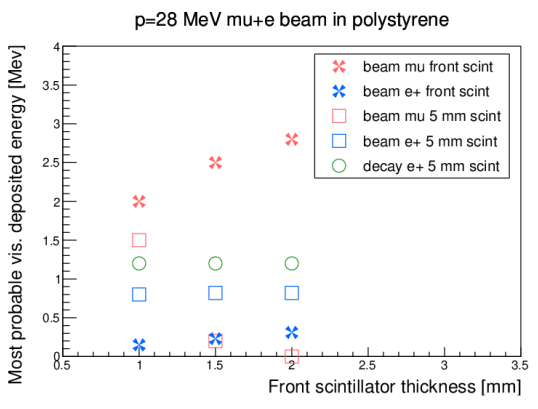
\includegraphics[width=0.5\linewidth]{Figures/muEDM/BeamMonitor/BeamMon_2mmScint_g4bl.png}
            \caption{Most probable visible deposited energy by muons and positrons in scintillators of various thicknesses, simulated in \textsc{G4beamline}. Muons and positrons with a momentum of \SI{28}{\MeVc} pass through a \SI{2}{mm}-thick front scintillator before reaching a \SI{5}{mm}-thick back scintillator. The green points are the decay positrons from muons stopped in the front scintillator.}
            \label{fig:BeamMonSimDepositedEn}
        \end{figure}
        
        \begin{figure}
            \centering
            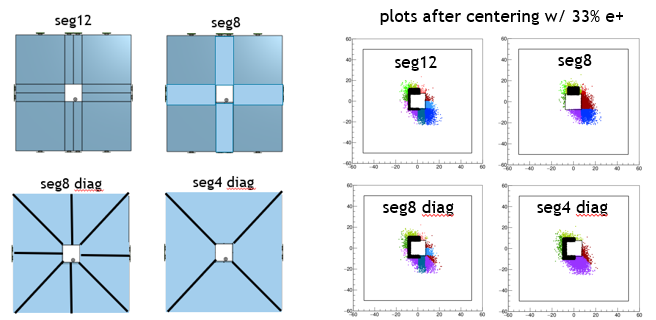
\includegraphics[width=0.8\linewidth]{Figures/muEDM/BeamMonitor/BeamMonConfigurations.png}
            \caption{Left: four geometries considered for the beam monitor. Right: Results of the beam centering in simulation, using the algorithm as described in the text, for the four geometries shown on the left image. Muon hits are colored differently based on which tile they hit, all positron hits are black.}
            \label{fig:BeamMonSimCentering}
        \end{figure}
        
        \begin{figure}
            \centering
            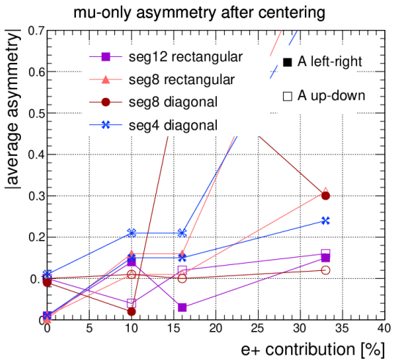
\includegraphics[width=0.4\linewidth]{Figures/muEDM/BeamMonitor/Mu+OnlyAsymm.png}
               \hspace{0.8cm}
            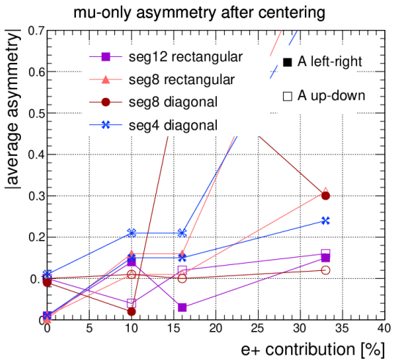
\includegraphics[width=0.4\linewidth]{Figures/muEDM/BeamMonitor/Mu-OnlyAsymm.png}
            \caption{Muon+positron (left) and muon-only (right) average asymmetries after the centering based on muon+positron counts. The asymmetries are plotted as a function of positron contribution in the beam.}
            \label{fig:BeamMonAsymmSim}
        \end{figure}
        
        
        \begin{figure}
            \centering
            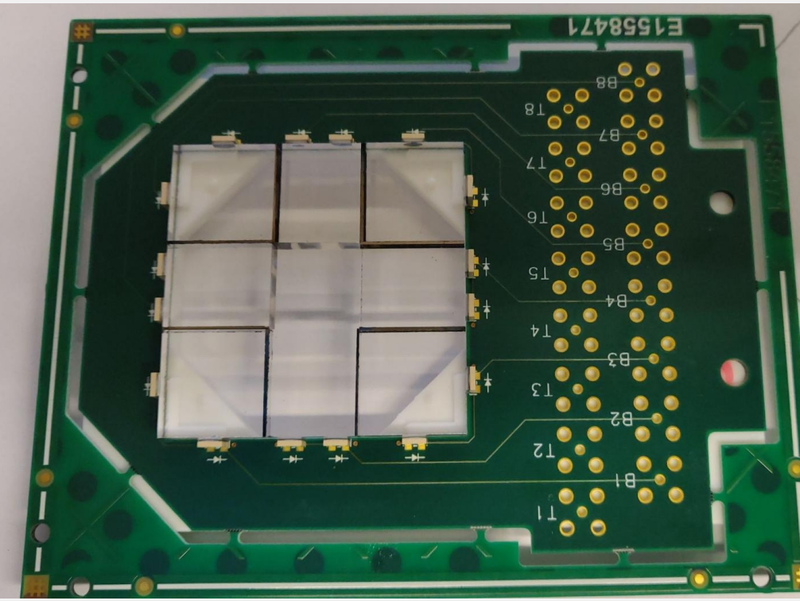
\includegraphics[width=0.4\linewidth]{Figures/muEDM/BeamMonitor/BeamMonRect.png}
            \hspace{0.8cm}
            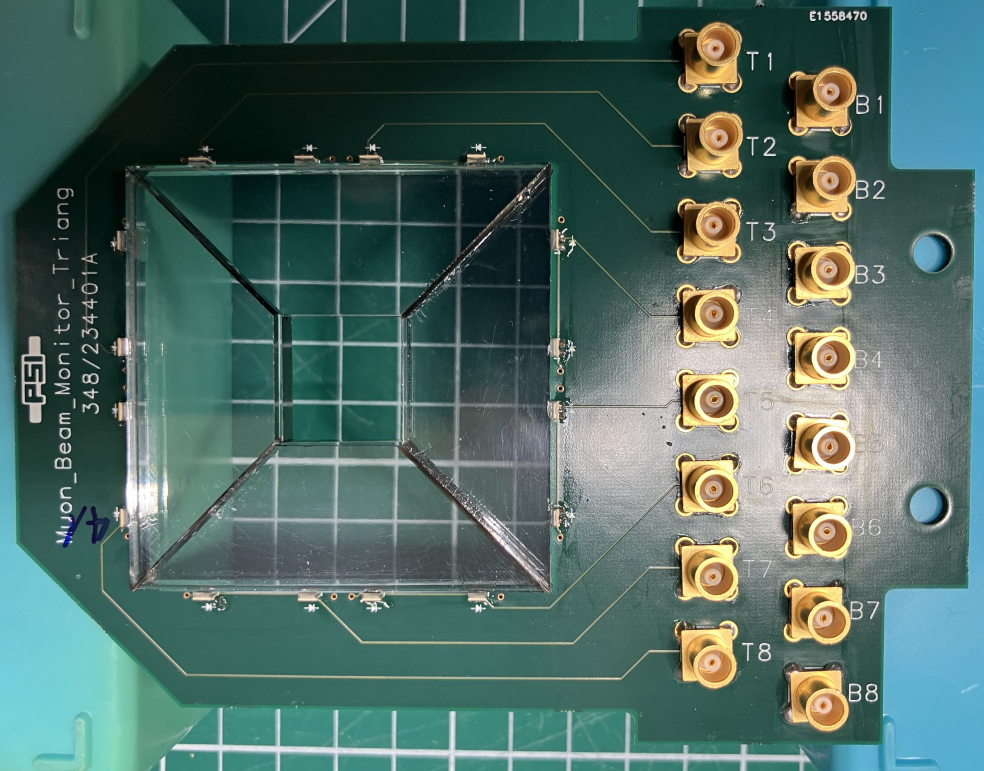
\includegraphics[width=0.4\linewidth]{Figures/muEDM/BeamMonitor/BeamMonTriang4.png}
            
            \caption{The two versions of the beam monitor during the assembly.}
            \label{fig:BeamMonAssembly}
        \end{figure}

    \status{review}
    \subsection{TOF}
        The accurate measurement of the muon Electric Dipole Moment (EDM) relies heavily on systematic effects control, which will be discussed in Sec.~\ref{sec:muEDM:systematics}. 
        The primary concern is the alignment of the electric field in the frozen-spin technique relative to the magnetic field defining the storage orbit. 
        To address this, a strategy involves alternating measurements with both clockwise (CW) and counter-clockwise (CCW) injected muons. 
        Switching from CW to CCW involves inverting the magnetic field and shifting the entire experiment by about \SI{90}{mm}, changing the magnetically shielded injection channel.
        
        The optimal cancellation of systematic effects requires identical initial conditions for the muon beam, like the spin phase and mean momentum. 
        Time of Flight (TOF) measurements for individual muons during injection enable the selection of CW and CCW datasets with nearly identical momentum distributions. 
        In 2023, prototype detectors were produced and TOF was measured in a test setup for alternating magnetic fields. 
        In 2024, the plan is to characterize the relative change in the initial muon spin after CW and CCW injection.
        
        The TOF detectors consist of thin Eljen Technology EJ-212 plastic scintillators coupled to Hamamatsu silicon photomultipliers. 
        Each detector has four channels, and their assembly details are shown in Fig.\ref{fig:muTOF_assemblyprocedure}. 
        The detectors aim for high detection efficiency (>95\%) and timing resolution (<\SI{1}{ns}). 
        Challenges include addressing the low number of collected scintillating photons due to the thin scintillator and handling a relatively high rate of thermal noise photon-electrons ($\sim$kHz). 
        The flexible detector design, with four independent channels, allows for optimal threshold triggering to achieve high detection efficiency and timing resolution.
        Additionally, a \gf-based Monte Carlo simulation aids in optimizing the detector design and complements data analysis.
        
        \begin{figure}
            \centering
            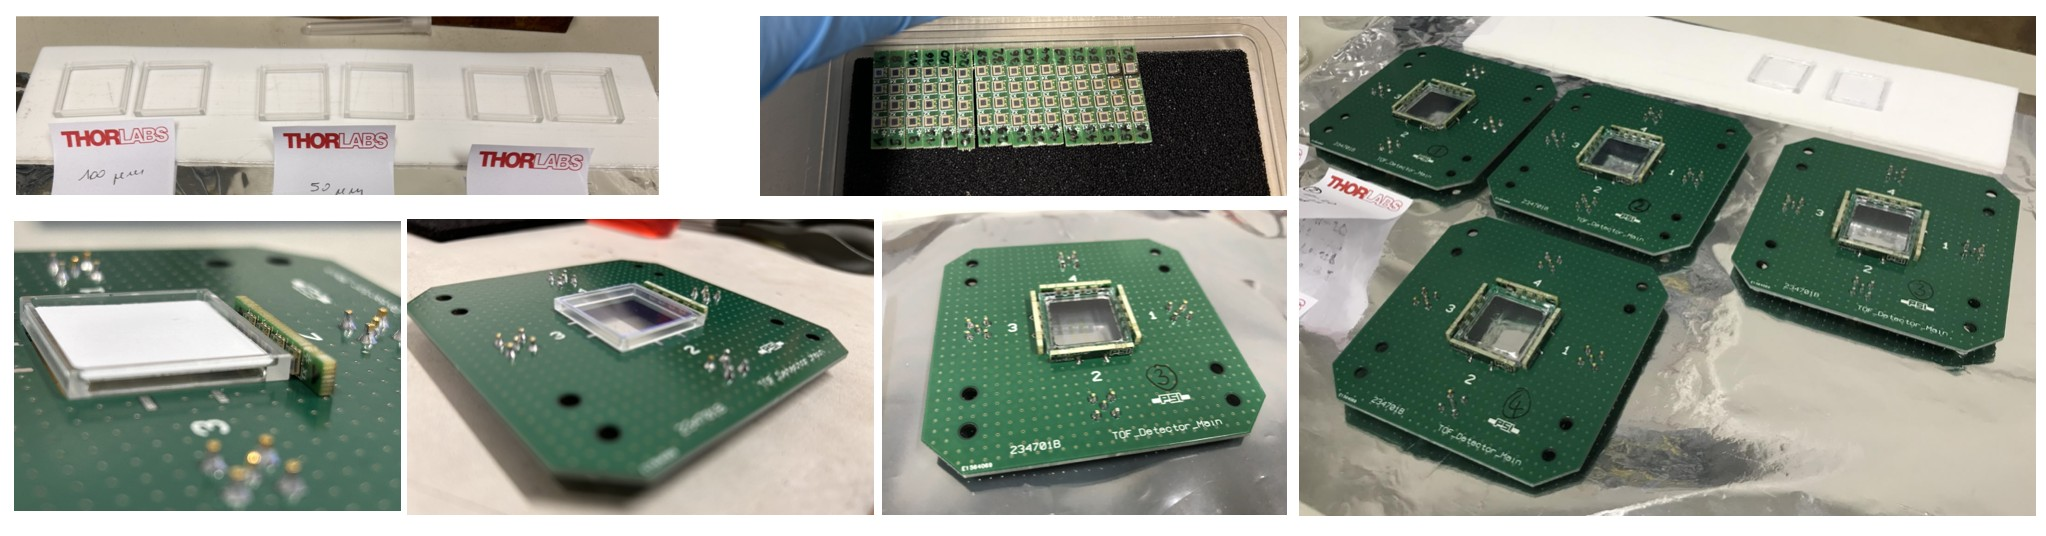
\includegraphics[width=16cm]{Figures/muEDM/muTOF_assembly.jpg}
            \caption{The TOF detectors during the assembly procedure. The scintillating windows during the gluing into the light guide (top left). The MPPC boards, where four MPPCs are soldered in series to form a single channel (top middle). A detail of the light guide (Bottom-right).}
        \label{fig:muTOF_assemblyprocedure}
        \end{figure}
        
    \status{review}
    \subsection{Entrance}
        To store muons at the center of the solenoid, a magnetic kick must be triggered at the right moment when the muon passes the weakly focusing field region. 
        An entrance detector, crucial for generating the trigger signal, consists of two thin scintillator tiles for CW and CCW injection and a thicker scintillator with openings around the nominal reference trajectory of the muon. 
        The trigger is initiated by the thin scintillator in anticoincidence with the thick one, reducing the required pulse rate of the kicker power supply from \SI{120}{kHz} to \SI{500}{Hz}. 
        Phase I entrance detector designs are under investigation \gf-based simulation tools, namely \textsc{musrSim} and \textsc{G4beamline}. 
        The CAD design of the entrance detector is shown in Fig.~\ref{fig:MuonEntranceTriggerCAD}.

        A fast electronic circuit is essential for the timely activation of the magnetic pulse, with simulation studies emphasizing the critical need for pulse latency within the \SI{120}{ns} to \SI{150}{ns} window. 
        Minimizing time delays throughout the system is crucial to meet these specifications.
        
        In 2023, data analysis from a test beam at PSI in late 2022 was conducted. 
        Two prototypes, featuring a thin entrance scintillator followed by a channel of four thick scintillators, all read out by SiPMs, were tested. 
        The measured results, particularly in terms of collected light, showed good agreement with simulations.
        The results of the simulations and the dedicated beamtimes will be discussed in Ch.~\ref{ch:muEDM:entrance}.
        Additionally, in Dic. 2023 new data, with a different readout scheme, were taken. 
        The preliminary analysis (and promising results) of these data will be also discussed.
        Based on these findings, ongoing work focuses on finalizing the design of the entrance detector for its intended functionality.

        \textcolor{red}{Dallo status report 2023 ho tagliato "Power supply for muon trigger electronics", "Pre-amplifier and splitter", "Discriminator". Forse vale la pena di aggiungere? Plus, Injection o Entrance?}

        \begin{figure}
        \centering
            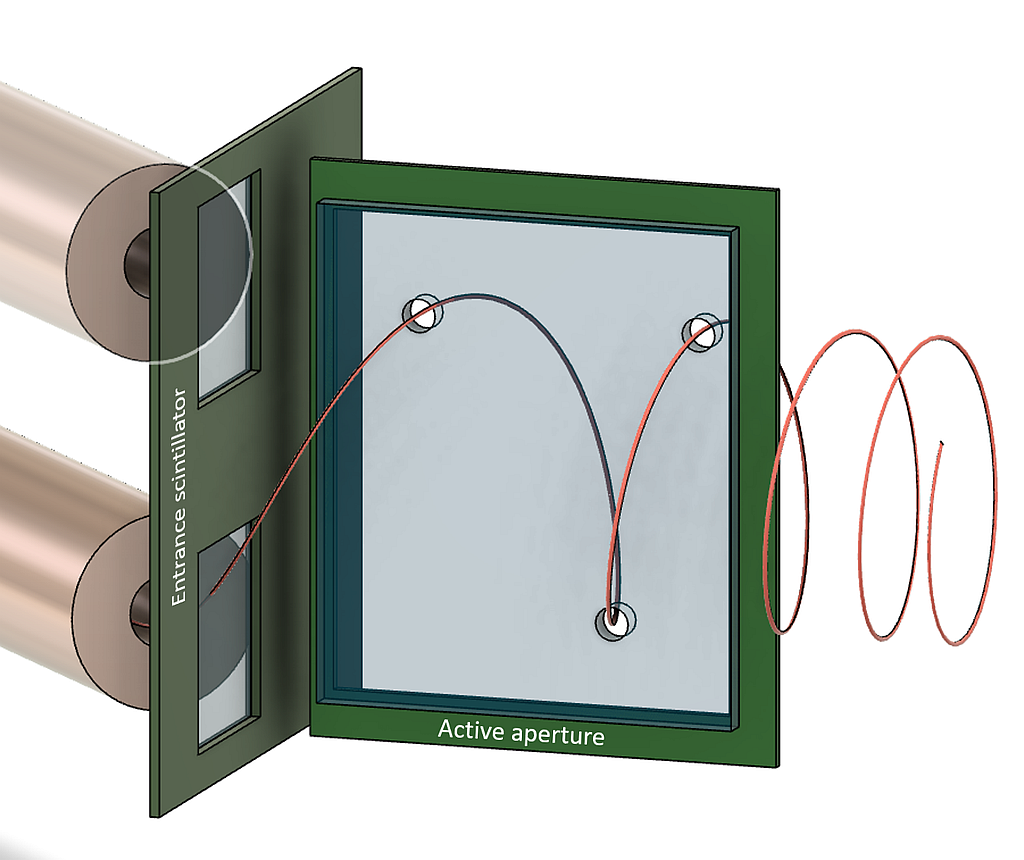
\includegraphics[width=0.35\linewidth]{Figures/muEDM/MuonEntranceTriggerCAD.png}
            \caption{CAD sketch of the entrance trigger. On the left, the muons exit the injection channel. The strong magnetic field immediately bends the muons onto a spiral trajectory. First, they pass through a thin ($\leq\SI{100}{\micro\meter}$) entrance scintillator. A thick second scintillator forms an active aperture, with holes at positions along the reference muon trajectory, which stops and detects muons that are outside the acceptance phase space. The trigger for the magnetic pulse, see Sec.~\ref{sec:muEDM:kicker}, will be generated by the anticoincidence of the two.}
        \label{fig:MuonEntranceTriggerCAD}
        \end{figure}

    \status{review}
    \subsection{Superconducting injection channel}
    \label{sec:muEDM:injection}
        To allow the incoming muons to enter the magnet without being reflected or deviated by fringing fields an injection channel is needed.
        For reasons that will be discussed in the section dedicated to the systematics (see Sec.~\ref{sec:muEDM:systematics}), we will actually require two symmetrical injections.
        The idea is to use a superconducting pipe: the fields around the pipe will generate Eddy currents which will, in turn, generate an opposite field inside the pipe, canceling the first.
        Clearly, the development of such a system is not trivial, and a precise study of the different shapes and materials is required. 
        The hope would be to find a suitable \textit{high-temperature} superconductor.

        \paragraph{Prototypes}
        Three different concepts for SC-prototype shields are currently being investigated and tested. 
        The first concept employs high-temperature superconducting (HTS) tape\footnote{2G HTS wire, S-Innovations, 2011-2020} made of Yttrium barium copper oxide~(YBCO), with a high $T_{\rm c}$ of \SI{93}{K}, wound helically around a copper tube. The second prototype consists of Nb-Ti/Nb/Cu SC-sheets~\cite{Barna2018}, with a $T_{\rm c}$ of \SI{9.2}{K}, clamped around a hollow copper tube. 
        Lastly, the third prototype will be a combination of a commercial SC-tube Bi-2223\footnote{CAN-superconductors, 2023}, with an inner diameter of \SI{15}{mm}, and a $T_{\rm c}$ between \SIrange{105}{110}{K}, and a stack of discs made of rare-earth barium copper oxide (REBCO)\@. 
        This approach benefits from isotropically induced currents in the Bi-2223 tube, as well as persistent currents along the circular paths in the disks.
        Once the SC-prototypes are assembled, we will test them and compare the shielding factor to results from numerical models using the finite element method (COMSOL) to identify the most efficient configuration with the highest shielding factor. 

        \paragraph{First tests}
        We are using a test setup made of a Helmholtz coil pair with a magnetic field strength of \SI{100}{mT} and a liquid nitrogen (LN\textsubscript{2}) bath maintained at \SI{77}{K} to evaluate the superconducting prototypes. 
        The SC prototype, under study, will be placed between the two coils and the whole system will be submerged in the cryogenic bath, as shown in Figure \ref{fig:Setup}.

        \begin{figure}
            \centering
            \subfloat[]{
            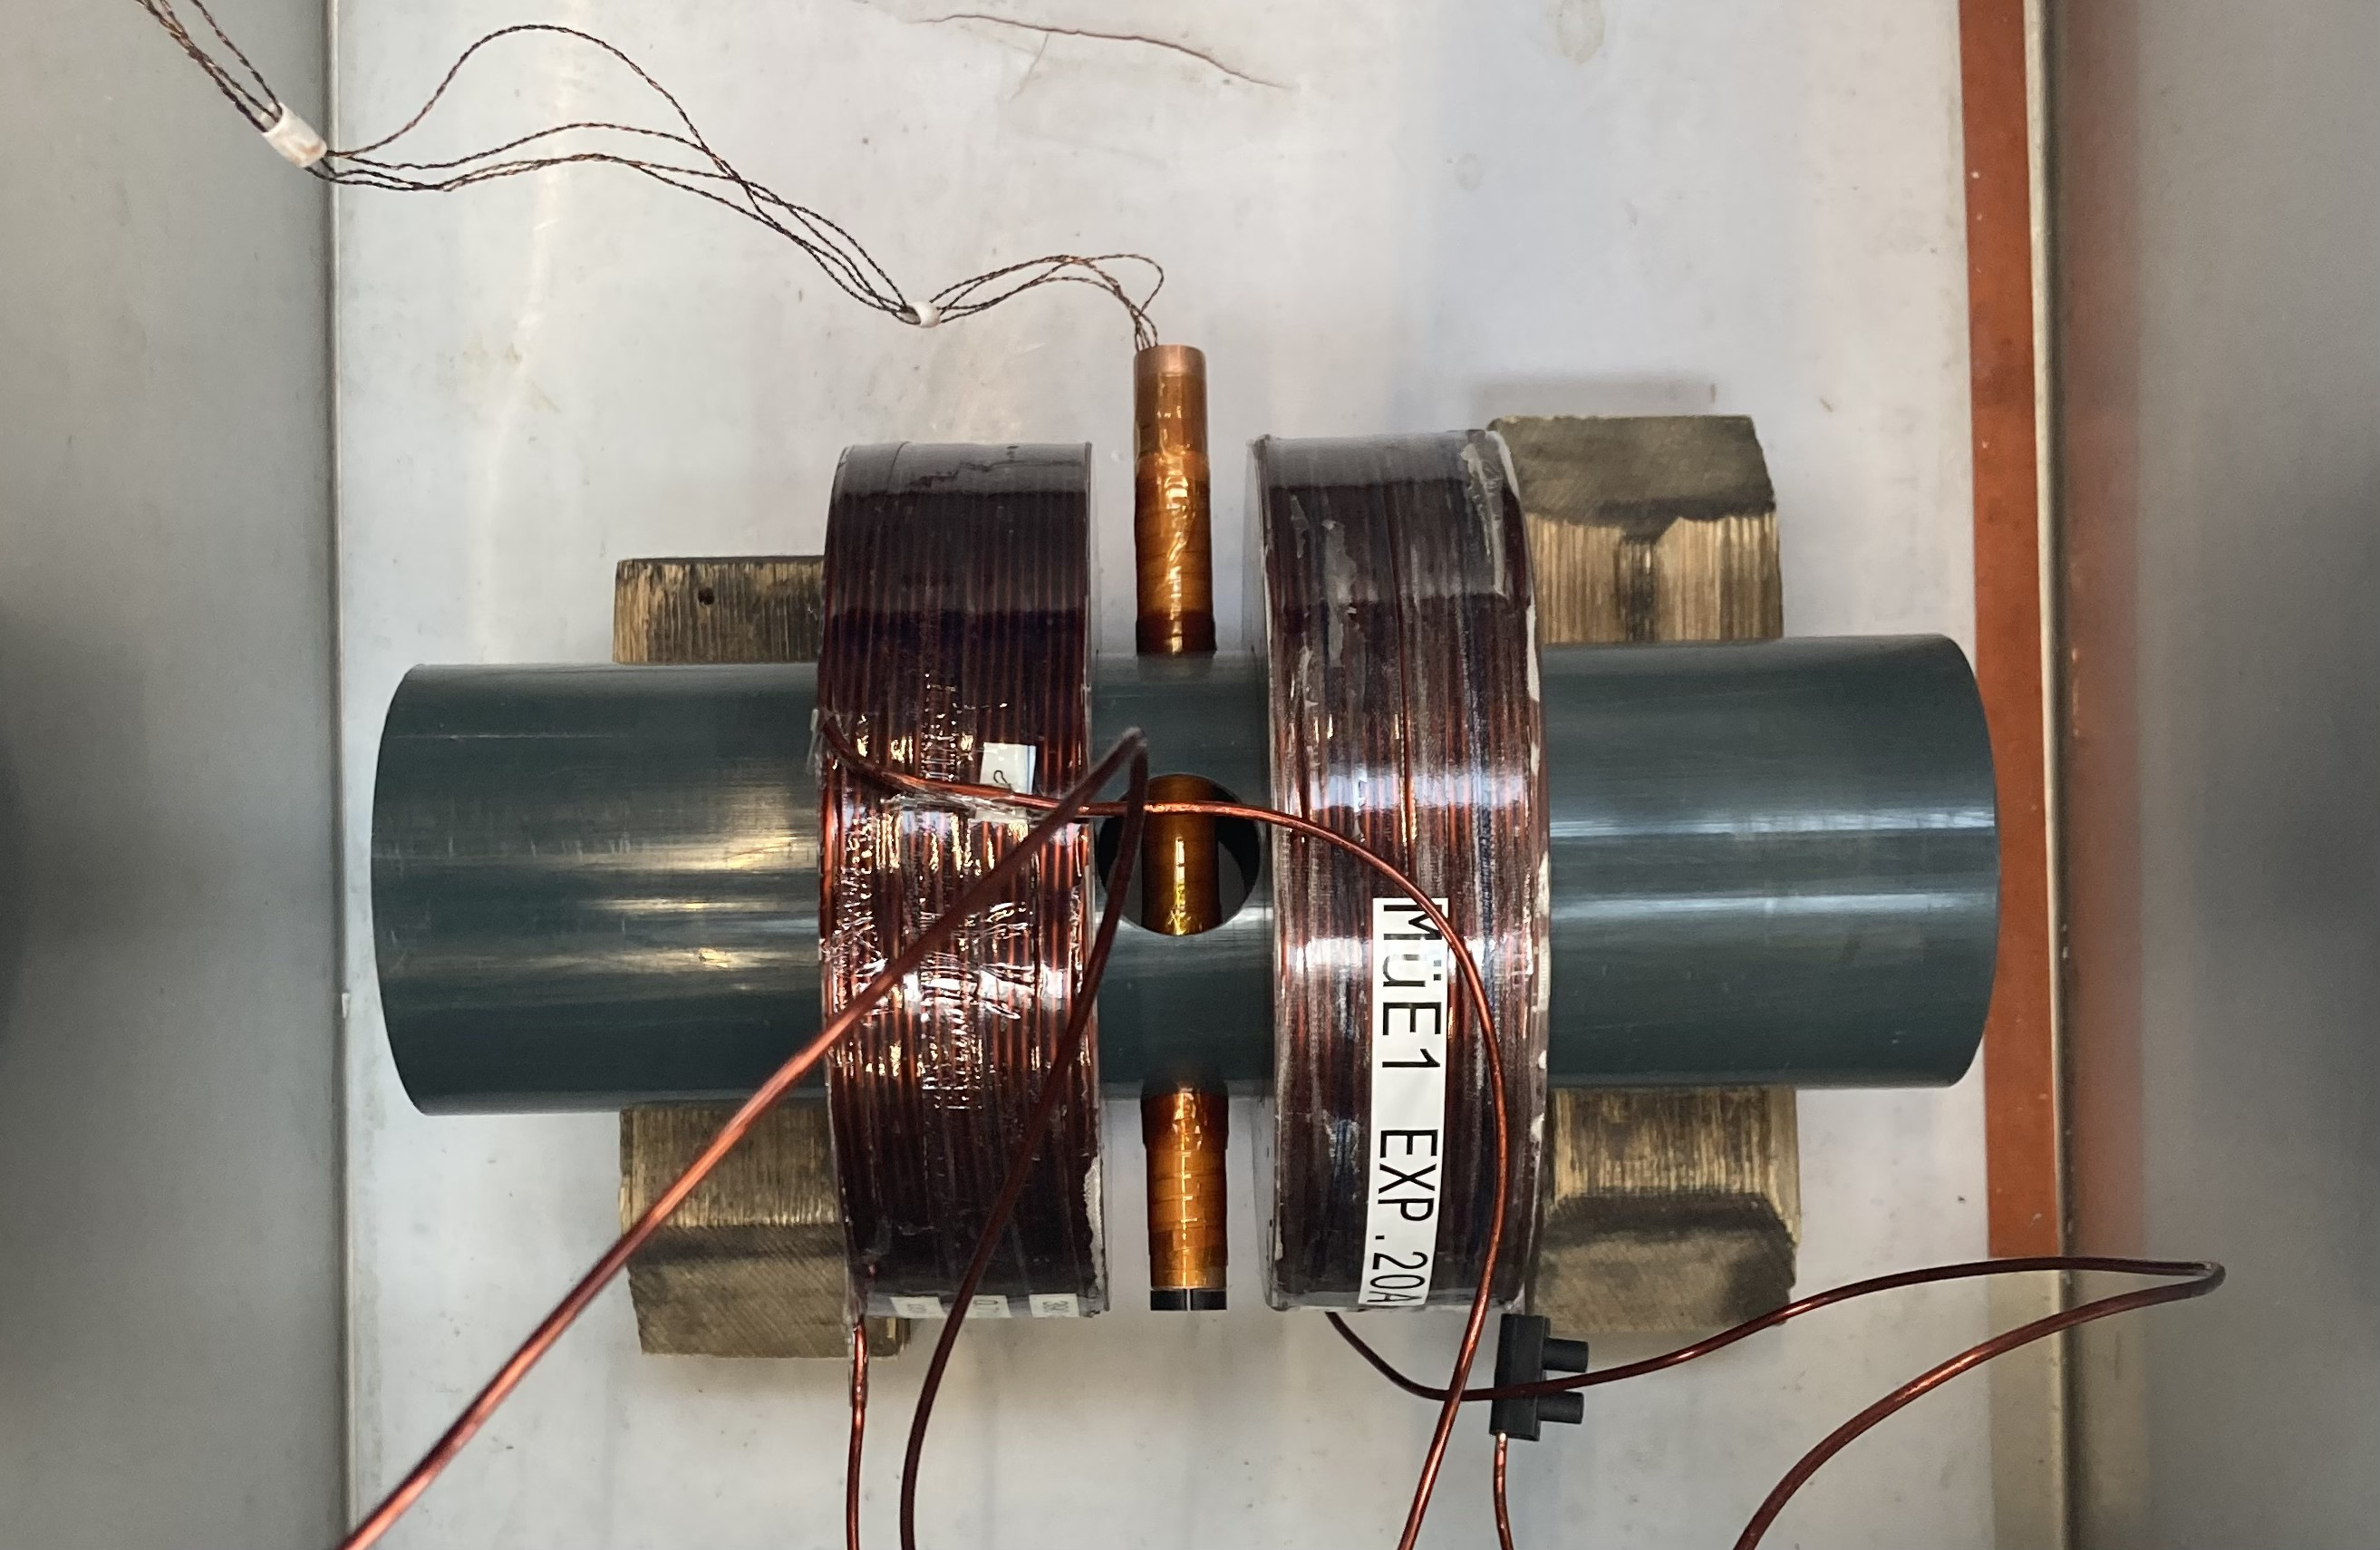
\includegraphics[width=0.5\columnwidth]{Figures/muEDM/SCshielding/SetUp.jpg}}
            \hfill
            \subfloat[]{
            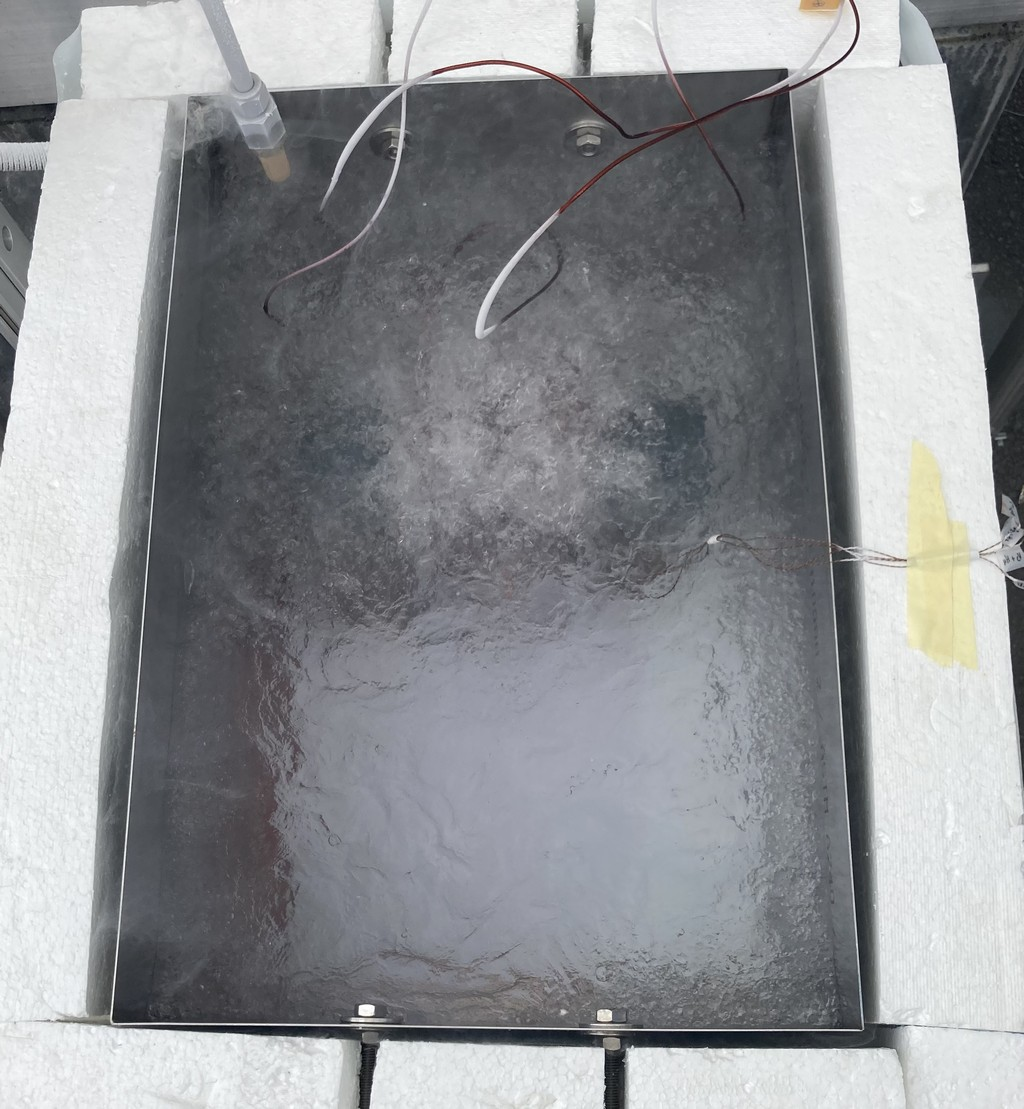
\includegraphics[width=0.3\columnwidth]{Figures/muEDM/SCshielding/IMG_8296.jpg}}
            \caption{(a)~Experimental setup for testing of superconducting shield prototypes; Helmholtz coil pair and a HTS-prototype placed between the two coils; (b)~setup submerged in LN\textsubscript{2}.}
        \label{fig:Setup}
        \end{figure}

        Initial measurements were performed on a prototype with a YBCO-tape, helically wound around a copper tube with an inner diameter of \SI{15}{mm} and a Bi-2223 sintered tube. 
        Measurements of the magnetic field inside the prototypes were conducted using four Hall sensors\footnote{THS119 Hall Sensors, TOSHIBA Electronic Devises \& Storage Corporation, 2023}, distributed along a 3D-printed support inside the tube on four positions with a separation of \SI{24}{mm} between each of them. 
        This setup enabled the measurement of the magnetic field as a function of position. 
        The measurements were taken at \SI{77}{K}, with and without superconducting shielding, as illustrated in Figures~\ref{fig:YBCO} and~\ref{fig:Bi2223}.

        \begin{figure}
            \centering
            \subfloat[]{
            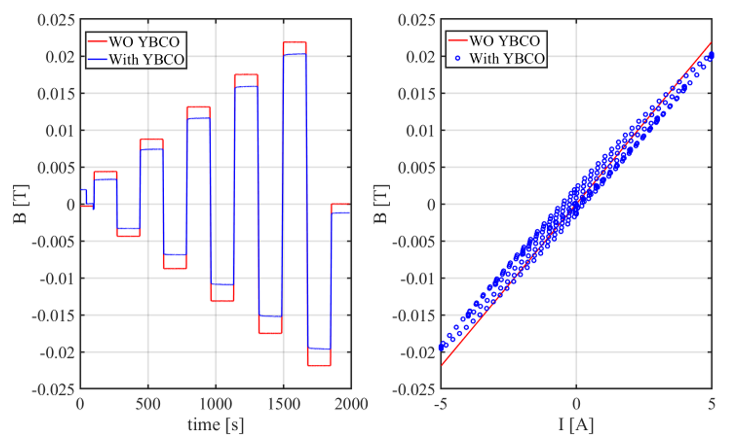
\includegraphics[width=0.58\columnwidth]{Figures/muEDM/SCshielding/YBCO_testMeasurements.png}}\hfill
            \subfloat[]{
            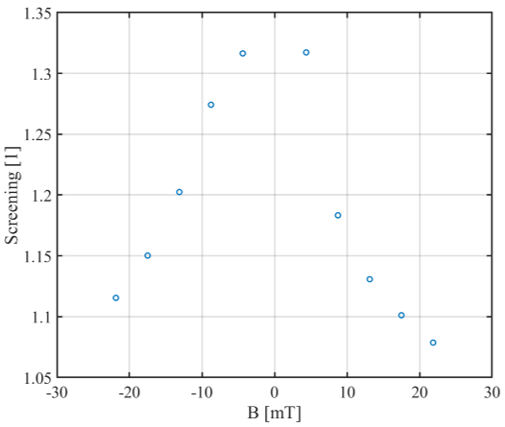
\includegraphics[width=0.40\columnwidth]{Figures/muEDM/SCshielding/YBCO_ScreeningFactor.png}}
            \caption{Measurement of the YBCO prototype. (a)~Measured magnetic field versus time, {\it left}, and versus coil current, {\it center}, at \SI{77}{K} with and without prototype. (b)~Shielding factor of YBCO prototype.}
        \label{fig:YBCO}
        \end{figure}
        
        \begin{figure}
            \centering
            \subfloat[]{
            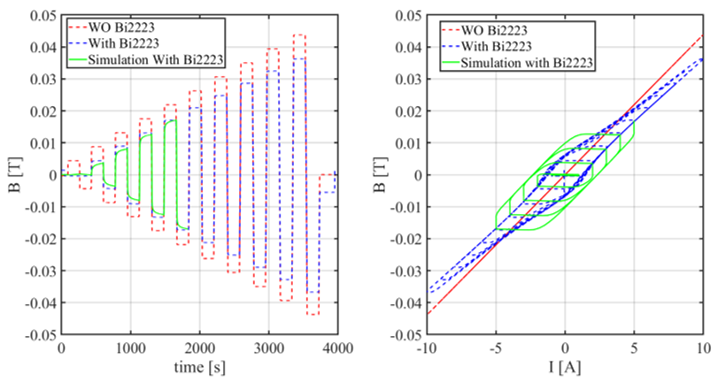
\includegraphics[width=0.62\columnwidth]{Figures/muEDM/SCshielding/Bi2223_testMeasurements.png}}\hfill
            \subfloat[]{
            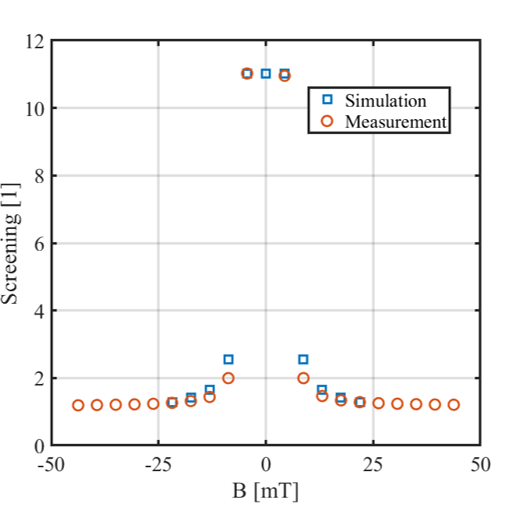
\includegraphics[width=0.34\columnwidth]{Figures/muEDM/SCshielding/Bi2223_ScreeningFactor.png}}
            \caption{Measurement of the Bi2223 prototype. (a)~Measured magnetic field versus time, {\it left}, and versus coil current, {\it center}, at \SI{77}{K} with and without prototype, and as simulated. (b)~Comparison of experimental versus simulated shielding factor of Bi2223 prototype.}
        \label{fig:Bi2223}
        \end{figure}

    \status{review}
    \subsection{Muon tracking}
    \label{sec:muEDM:gridpix:beamtime}
        Although during physics runs it is important to minimize the number of interactions of the muon along the path, it is a cardinal step to prove the muons are following the correct path and are properly stored.
        On top of this, the momentum difference between the CW and CCW injection needs to be below 0.5\%.
        For this reason, a removable muon-tracking device is under development.
        The proposed solution is a Time Projection Chamber (TPC) operated with an extremely light gas mixture based on helium, separated from the vacuum in the magnet bore by an extremely thin and vacuum-tight window (\SI{300}{\nano\meter} Silicon Nitride). 
        As a readout structure for this \tpc, the \grid detector is considered. 
        \grid is a gaseous detector made of a conductive mesh implanted \SI{50}{\micro\meter} above a Timepix chip~\cite{Llopart2007NIMA}.
        A voltage difference between the mesh and the chip produces an avalanche when drift electrons reach the mesh so that the \grid behaves like a sort of microscopic Micromegas.

        \paragraph{Beamtime}
        A prototype of this detector was developed with a single GridPix and flushed with helium-isobutane gas mixtures. 
        It was tested in 2022, and the results have been published and can be found in \cite{muEDM:PSI:GridPix}.
        The setup was quite simple: the beam was centered through the TPC and scintillators were used as an external trigger.
        During this testing, the detector was tested at different pressures and voltages, and with different mixtures of gas.
        In Fig.~\ref{fig:gridpix_plateau} the trend of the detection efficiency of GridPix as a function of the mesh voltage is shown, demonstrating that the detector can be used with these kinds of mixtures with a wide efficiency plateau.
        In Fig.~\ref{fig:tpc_reso} the reconstructed momentum and phase space.\\

        \begin{figure}
            \centering
            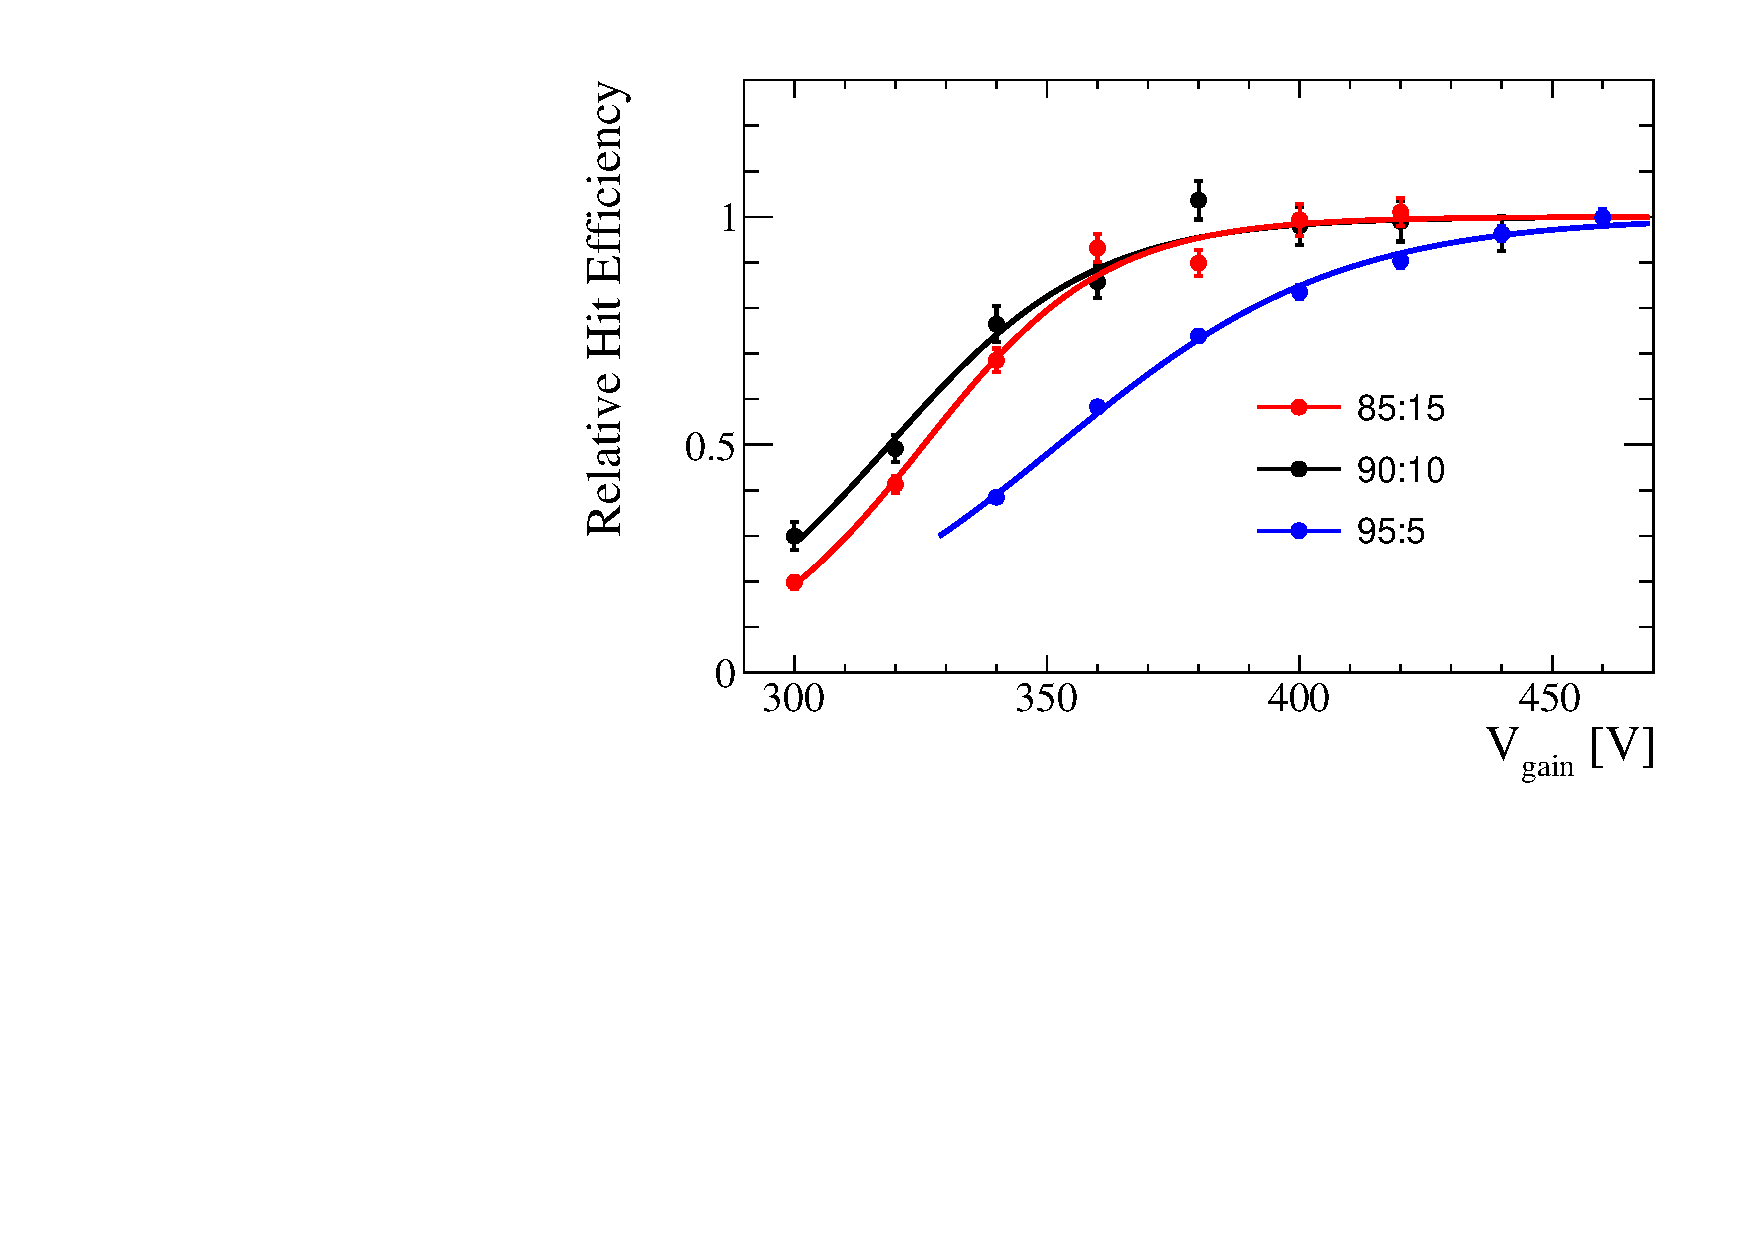
\includegraphics[width=0.5 \linewidth]{Figures/muEDM/gridpix_plateau.pdf}    
            \caption{Average number of reconstructed hits per track in the GridPix detector, as a function of mesh voltage, normalized to the asymptotic value of a sigmoid curve fitting the data points, for three different mixtures of helium-isobutane (95:5, 90:10, and 85:15).}
            \label{fig:gridpix_plateau}
        \end{figure}
        
        \begin{figure}
            \centering
            \subfloat[]{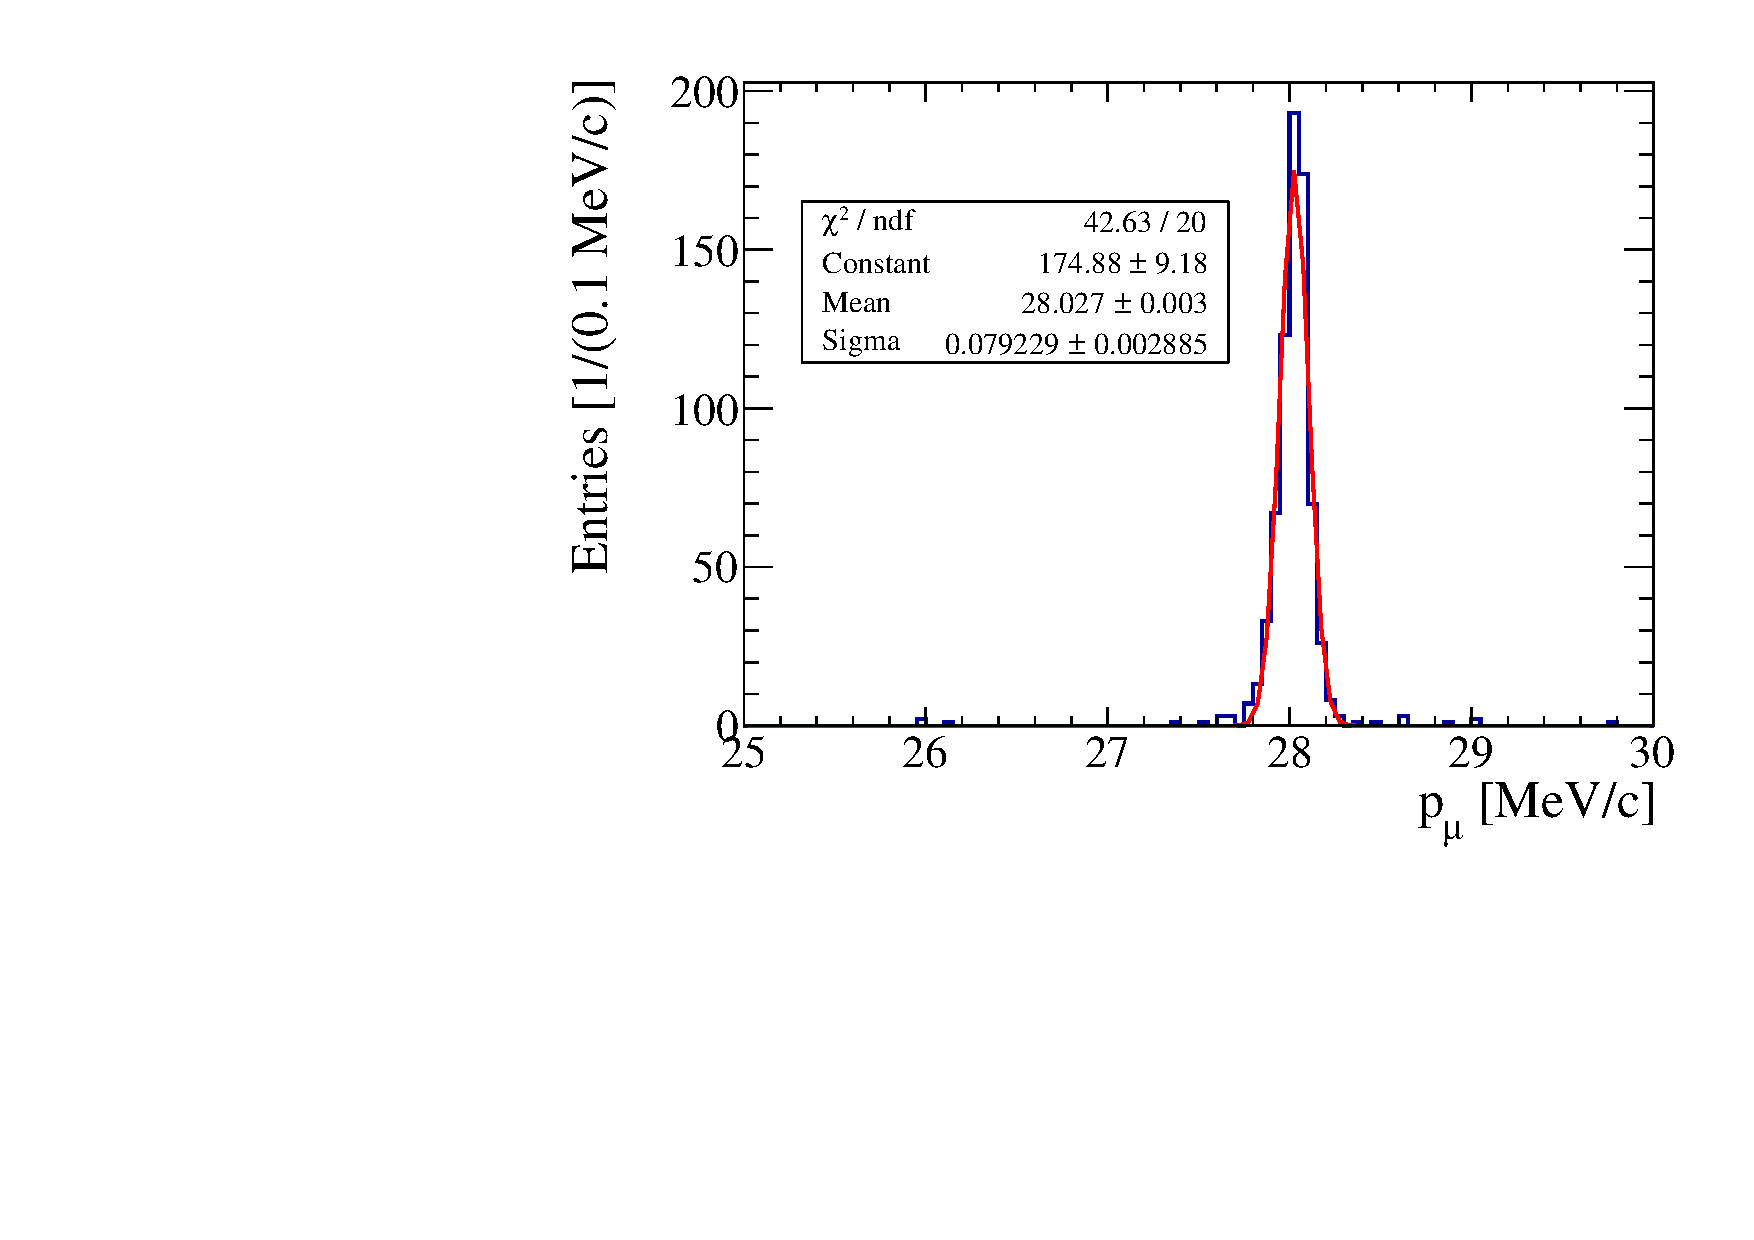
\includegraphics[width=0.5\linewidth]{Figures/muEDM/momentum_long_0.4.pdf}
            }
            \subfloat[]{
            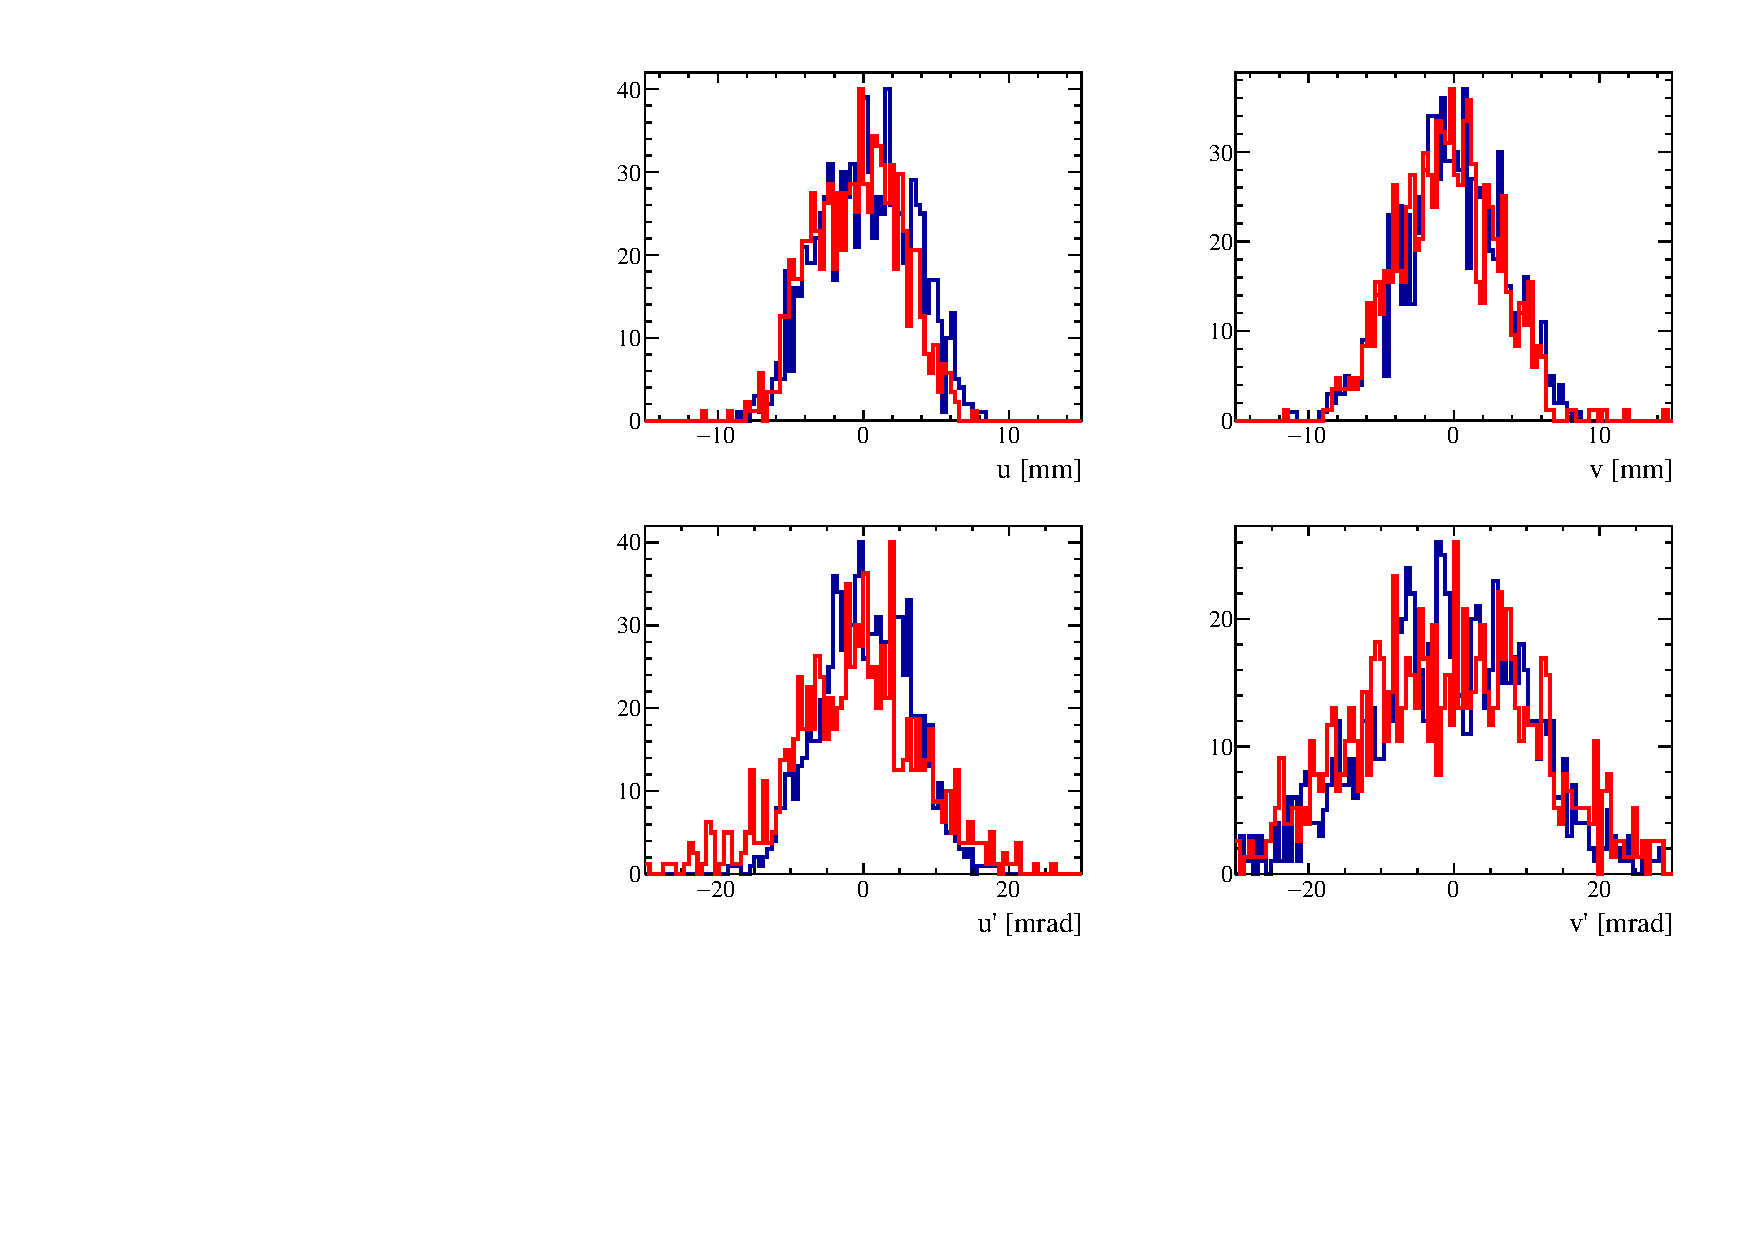
\includegraphics[width=0.45\linewidth]{Figures/muEDM/phase_space_long_0.4.pdf}
            }
            \caption{Performance of a longitudinal TPC for the reconstruction of injected muons. (a) Reconstructed momentum (assuming \SI{28}{MeV/c} initial momentum). (b) True (blue) and reconstructed (red) phase space coordinates and angles (u: horizontal; v: vertical).}
        \label{fig:tpc_reso}
        \end{figure}
        
        \noindent
        Following a successful beam test, simulation studies were conducted to evaluate the tracking capabilities of a Time Projection Chamber (TPC) designed for tracking \SI{28}{MeV/c} muons within the Phase~I magnet. 
        Two geometries were explored: a conventional longitudinal setup, where electrons drift along the $z$ axis parallel to the magnetic field, and an unconventional radial configuration, with electron drift in the $(x,y)$ plane. 
        Typically, TPC track resolution is highest in the direction orthogonal to the drift, favoring the longitudinal option for optimal momentum resolution, while the radial geometry excels in measuring muon entrance angles. 
        Despite assuming a detector pressure of \SI{400}{\milli\bar} in the simulations, the prevalence of multiple scattering effects diminishes the characteristic differences between the two geometries, making the resolution advantages less distinct.
        Achieving a momentum resolution surpassing \SI{0.3}{\percent} appears feasible, and the phase space resolutions seem adequate for alignment purposes. 
        In early 2024, a decision will be made regarding the TPC configuration, and the detector engineering will be finalized by year-end. 
        This encompasses the development of mechanical mockups for installing silicon nitride entrance windows with a thickness of \SI{300}{\nano\meter}. 
        On the detector front, tests are scheduled to experimentally validate the proposal to operate the detector at sub-atmospheric pressure, considering the anticipated very high ionization rates in the Phase~I experiment. 
        The design process will be complemented by thorough simulation studies aimed at optimizing the final configuration.
        
    \status{review}
    \subsection{Kicker}
    \label{sec:muEDM:kicker}
        The prerequisite for the \textit{frozen spin} is to first store the muon around the design orbit.
        This is achieved by applying a longitudinal kick, canceling the momentum component parallel to the magnetic field.
        The development of this element is non-trivial because of the stringent requirements on the strength, time scale, and residual effects of the kick.
        A weakly focusing static field, produced by a circular coil, ensures confinement. 
        To compensate for muon acceleration upon entering the weakly focusing field, the pulsed field must be optimized to reduce longitudinal oscillations.
        The trigger signal for the magnet pulse, generated by the entrance detector previously discussed, selects muons within the storage phase space. 
        Considering processing delays, the \textit{on-demand} pulse generator must have an internal latency <$\SI{60}{ns}$.
        
        The Institute for Pulsed Power and Microwave Technology at KIT developed high-voltage switching technology \cite{GateBoosting}, meeting current pulse specifications. 
        The generator, designed with a \SI{20}{\micro s} recovery time, can deliver up to 2000 pulses per second. 
        Pulse amplitude and shape are defined passively by load circuit impedance characteristics. 
        Lower inductance, achieved by splitting pulse coils into quadrants supplied in parallel, allows operation at \SI{12}{kV}, supporting the required pulse width and reducing voltage ratings of components and cables.

        \paragraph{Prototype}
        A \SI{100}{\micro m} copper sheet prototype for the quadrant pulse coil configuration (Fig.~\ref{fig:coils}(a)) was constructed, minimizing positron multiple scattering compared to \SI{500}{\micro m} thick plastic scintillating fibers. 
        The measured inductance per loop was \SI{76(3)}{nH}, in line with the ANSYS model prediction of \SI{79}{nH}.
        
        ANSYS-generated field maps (Fig.\ref{fig:coils}(c) and(d)) simulated the kick and characterized field strength and inductance. The quadrant model's geometry (Fig.\ref{fig:coils}(b)) with overlapping longitudinal sections led to partial cancellation due to opposite polarities. The DC magnetic field map in the central ($z=0$) $x-y$-plane is shown in(c), and plot~(d) displays the field along the orbit, parameterized by azimuthal angle $\phi$.
        
        The orange line at \SI{8.4}{\micro\tesla\per\ampere} in plot~(d) represents the average field strength over the orbit, falling $20\%$ below the expected strength for ideal circular loops. 
        Despite requiring a higher current for a given field strength, the quadrant model's advantage lies in the shorter pulse width allowed by low-inductance parallel circuits. 
        The compact design minimizes stray capacitance and inductance. 
        Supplying upstream and downstream segments in series within each quadrant ensures better longitudinal symmetry of the field, with equal current flow in both segments.
        
        \begin{figure}
        \centering
            \subfloat[Coil quadrants prototype]{
            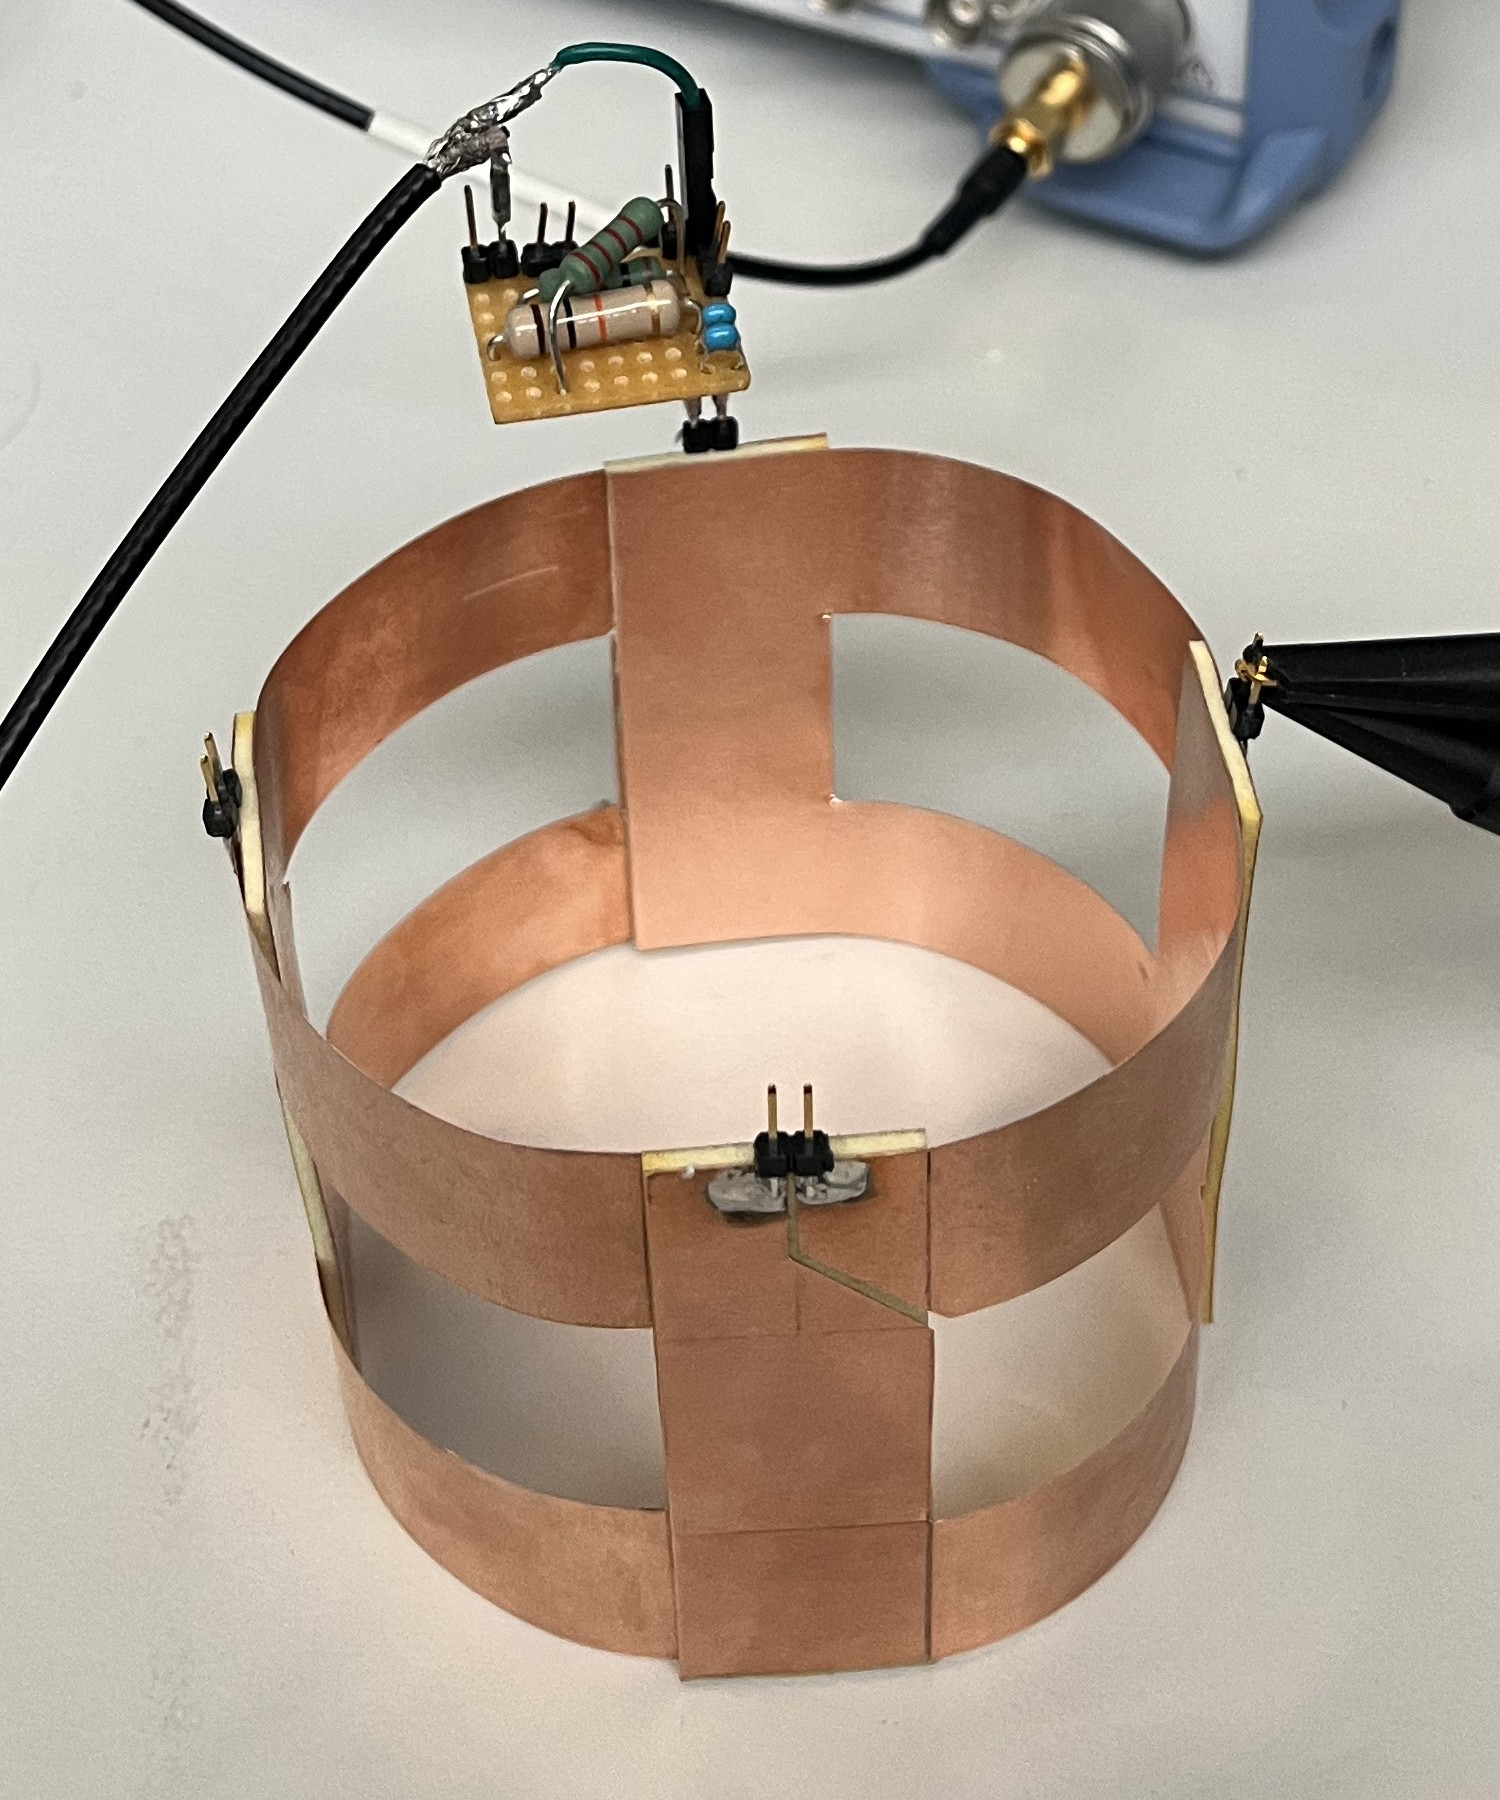
\includegraphics[width=0.27\textwidth]{Figures/muEDM/Pulser/quadprototype.jpg}}
            \hfill
            \subfloat[Quadrant geometry (ANSYS)]{
            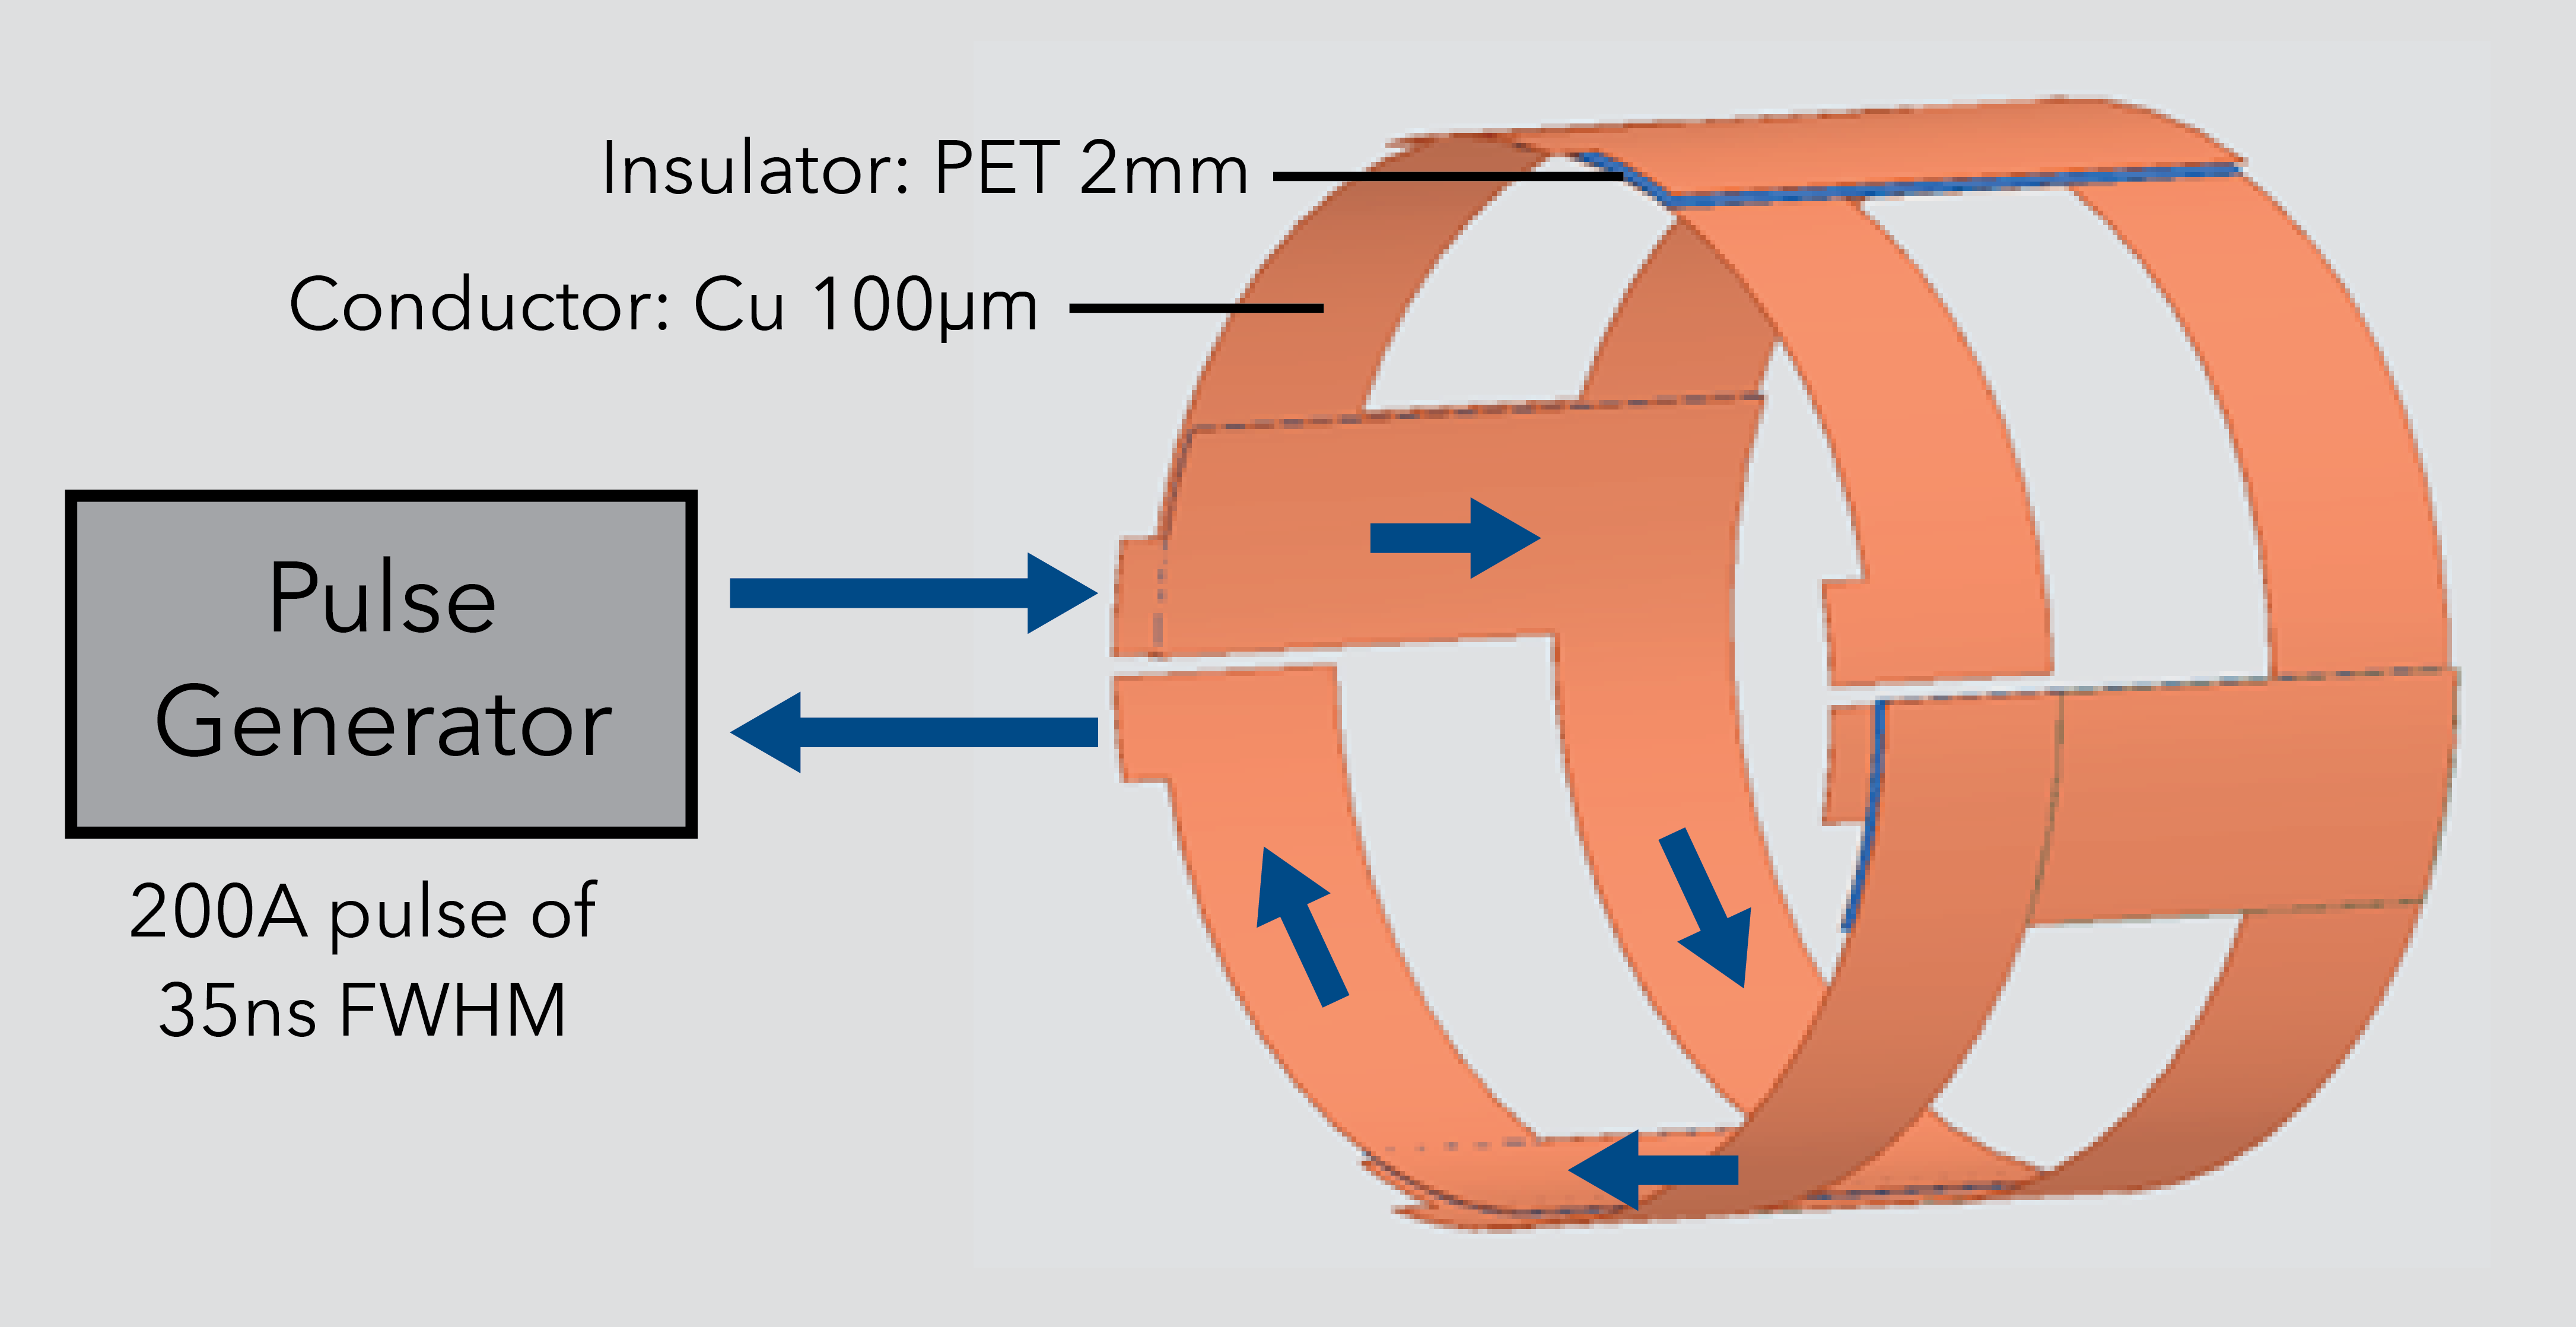
\includegraphics[width=0.65\textwidth]{Figures/muEDM/Pulser/ANSYS_Geometry.png}}
            \hfill
            \subfloat[Magnetic field map (z=0)]{
            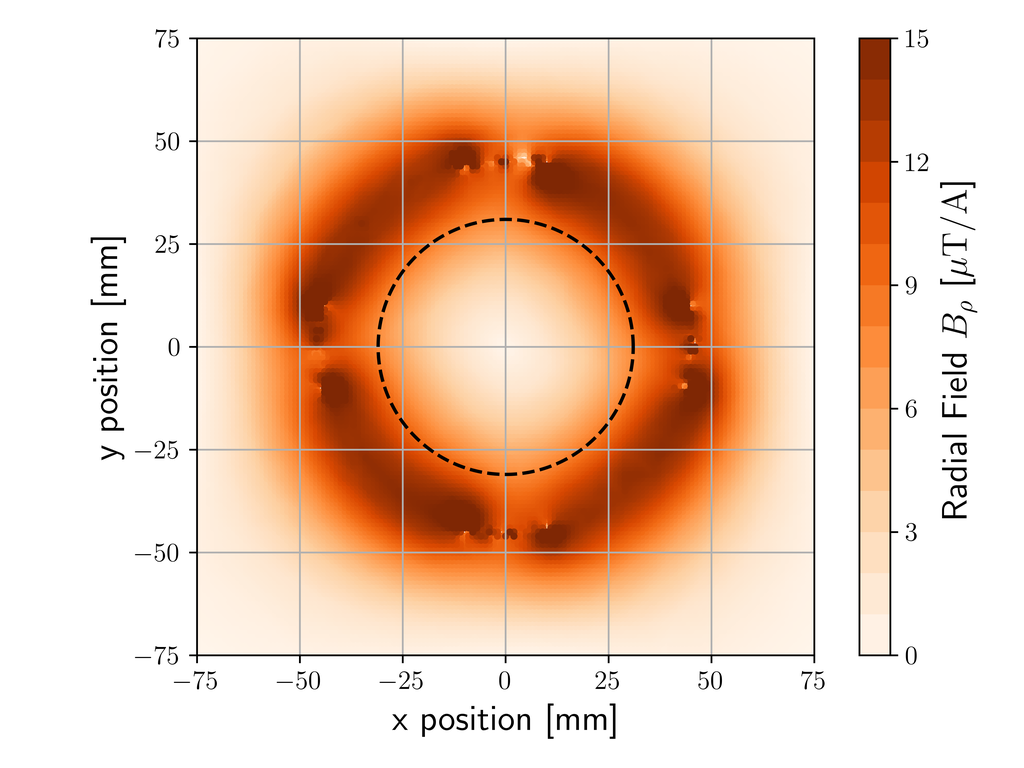
\includegraphics[width=0.45\textwidth]{Figures/muEDM/Pulser/xy0map.png}}
            \hfill
            \subfloat[Magnetic field along orbit]{
            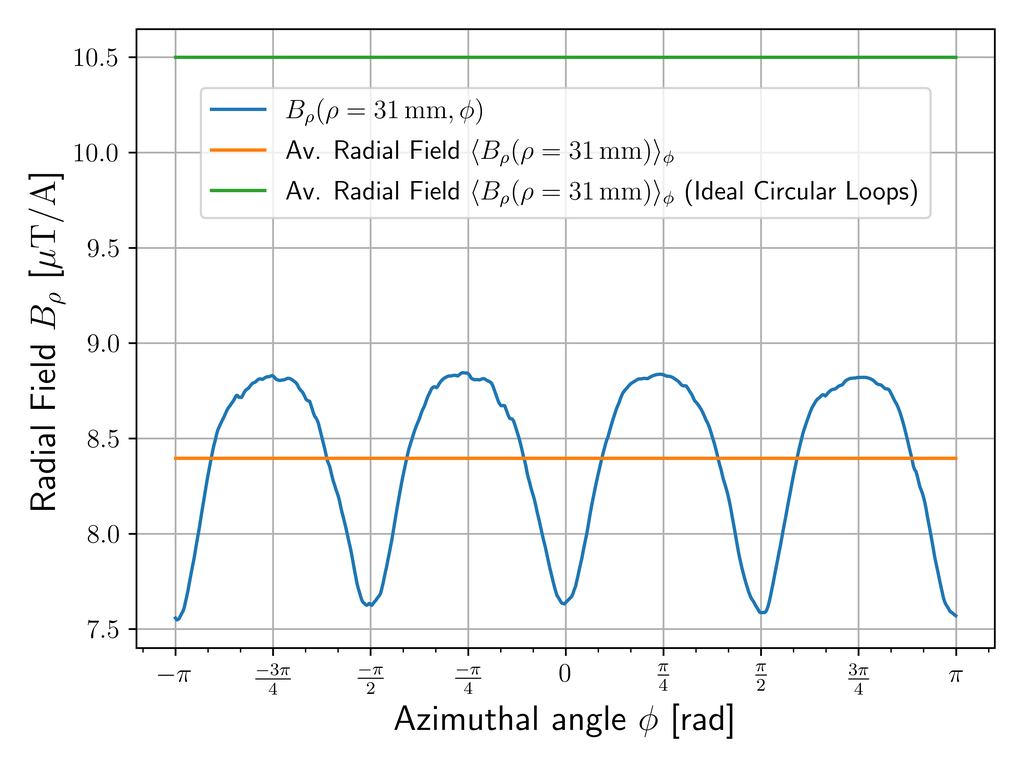
\includegraphics[width=0.45\textwidth]{Figures/muEDM/Pulser/xyint0map.png}}
            \caption{The pulse coils, (a)~prototype and (b)~geometry implemented in ANSYS, are responsible for kicking the remaining longitudinal momentum to permit storage in a weakly-focusing magnetic field. 
            They will be constructed from \SI{100}{\micro m} copper sheets to minimize multiple scattering without significantly increasing electrical resistance for frequencies $\sim \SI{10}{\mega\hertz}$.
            The ANSYS simulation produces field maps, shown on the central $x-y$-plane in~(c) where the dashed black line shows the stored muon orbit. 
            The average field strength over the orbit is \SI{8.4}{\micro\tesla\per\ampere}, as shown by the orange line in~(d), where the field strength is plotted over the orbit parametrized by the azimuthal angle $\phi$.}
        \label{fig:coils}
        \end{figure}
        
        \paragraph{Generator}
        The pulse generator design, developed in collaboration with the KIT team, adheres to constraints from injection simulations and systematic effects studies. 
        Operating at \SI{12}{kV}, it delivers \SI{200}{A} to each coil quadrant. 
        Load characteristics, shaping the pulse, are defined based on prototype measurements and ANSYS simulations. 
        Inductive couplings between parallel circuits are determined from induced voltage measurements on the prototype.
        
        The current design, shown in Fig.~\ref{fig:circuit} includes resistance-capacitive~(RC) damping elements on the coaxial cable, tuned to critically damp the primary pulse and suppress after-pulse oscillations. 
        This avoids perturbing the muon orbit or inducing time-dependent spin precession signals. 
        The pulse shape, influencing the applied momentum kick, is adjustable to maximize storage efficiency. 
        Simulated current profiles, shown in Fig.~\ref{fig:pulses}, illustrate optimized damping for maximizing peak current and reducing after-pulse oscillations. 
        The voltage over the charging capacitor \textit{C1} demonstrates recovery within $1\%$ of the nominal operating voltage after a \SI{20}{\micro s} delay, meeting the desired interval between muon triggers.
        We plan to commission and test the pulse generator in mid-2024 for the upcoming beam test. 
        The circuit parameters are being finalized, while a full load circuit characterization, utilizing a network analyzer, is ongoing to refine the ANSYS model of the quadrant configuration.
            
        \begin{figure}
            \centering
            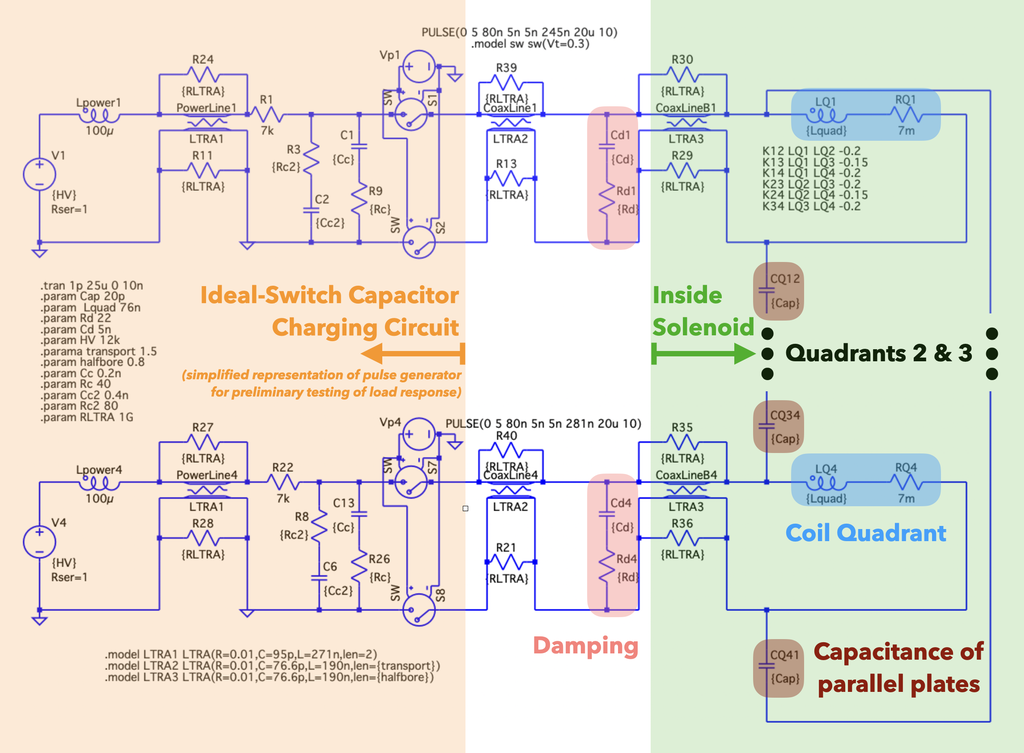
\includegraphics[width=\textwidth]{Figures/muEDM/Pulser/PulserModelJan2024.png}
            \caption{Circuit model, developed in LTSpice, for the load attached to simplified charging-stage circuits using ideal switches. Transmission lines labeled \textit{CoaxLine1-4} transmit from generator to the external flange of the solenoid; \textit{CoaxLineB1-4} transmit from the flange to the center of the bore, where the coils are located. Inductive couplings between quadrants \textit{i} and \textit{j} are specified by the listed constants labeled \textit{Kij}. Capacitive couplings between quadrants \textit{i} and \textit{j} are described by capacitors labeled \textit{CQij}. The second and third quadrants are not shown for compactness.}
        \label{fig:circuit}
        \end{figure}
        
        
        \begin{figure}
        \centering
        \subfloat[Pulse current]{
        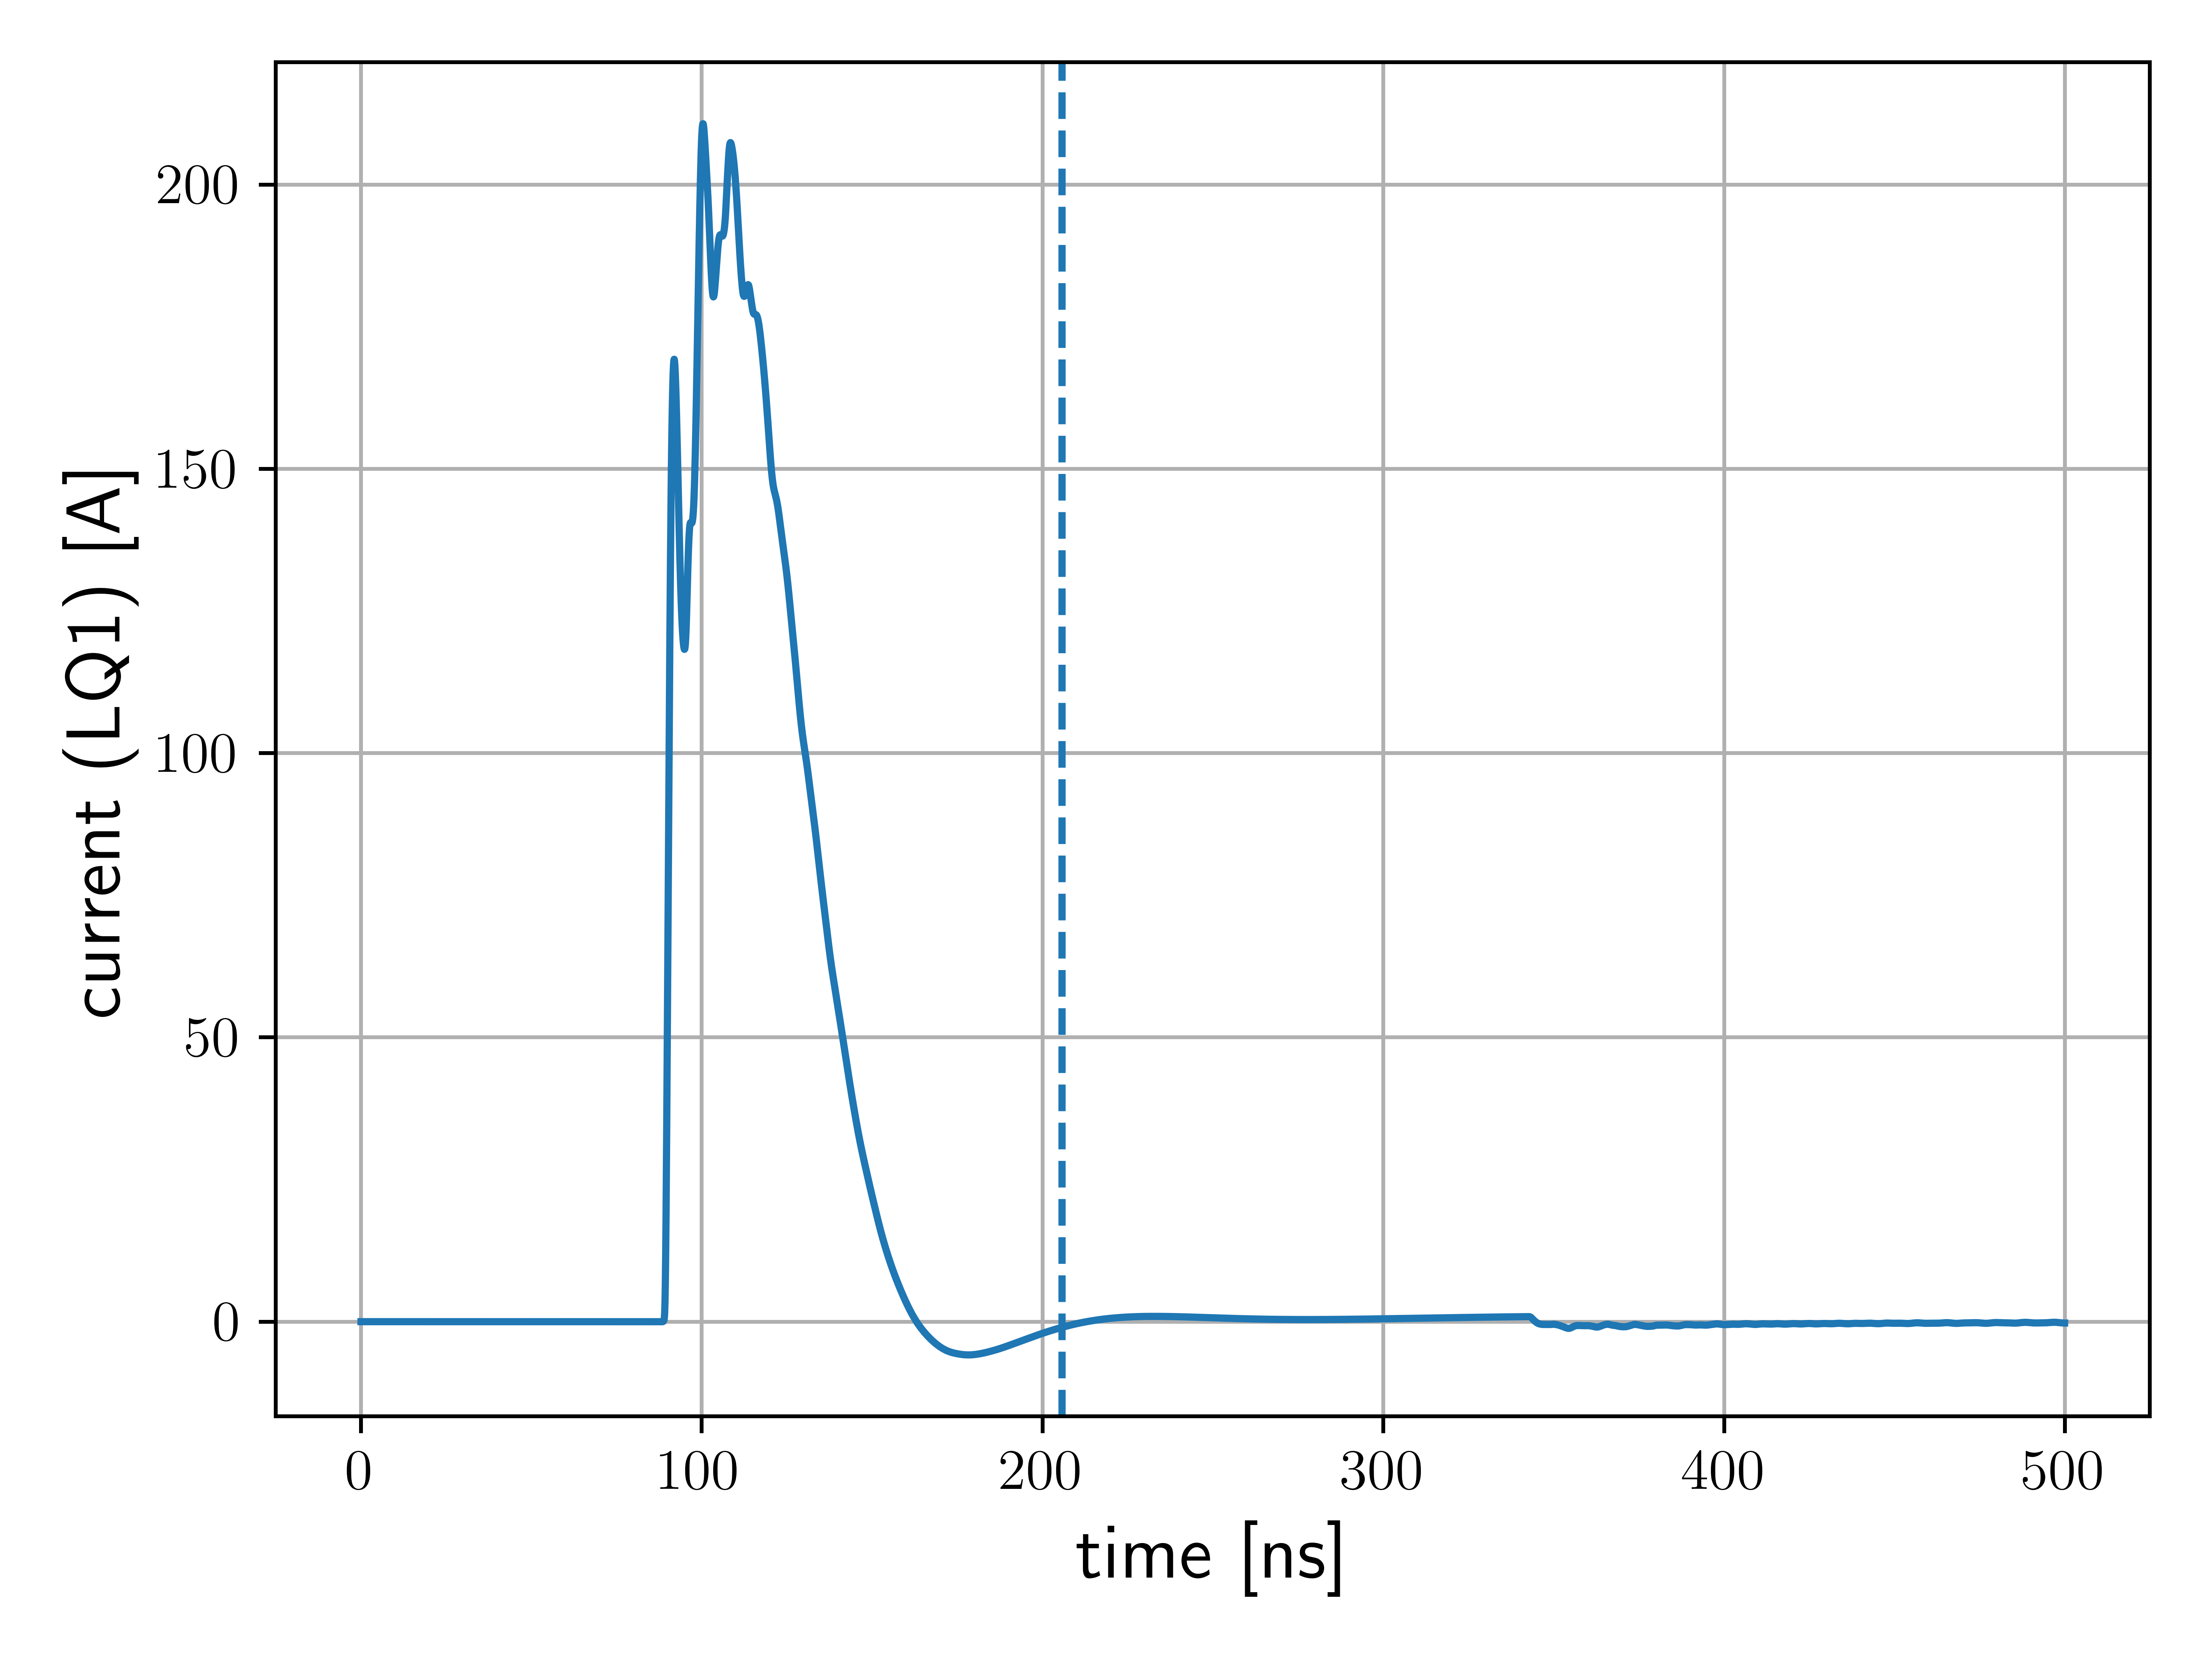
\includegraphics[width=0.3\textwidth]{Figures/muEDM/Pulser/pulse.png}}
        \hfill
        \subfloat[After-pulse oscillations]{
        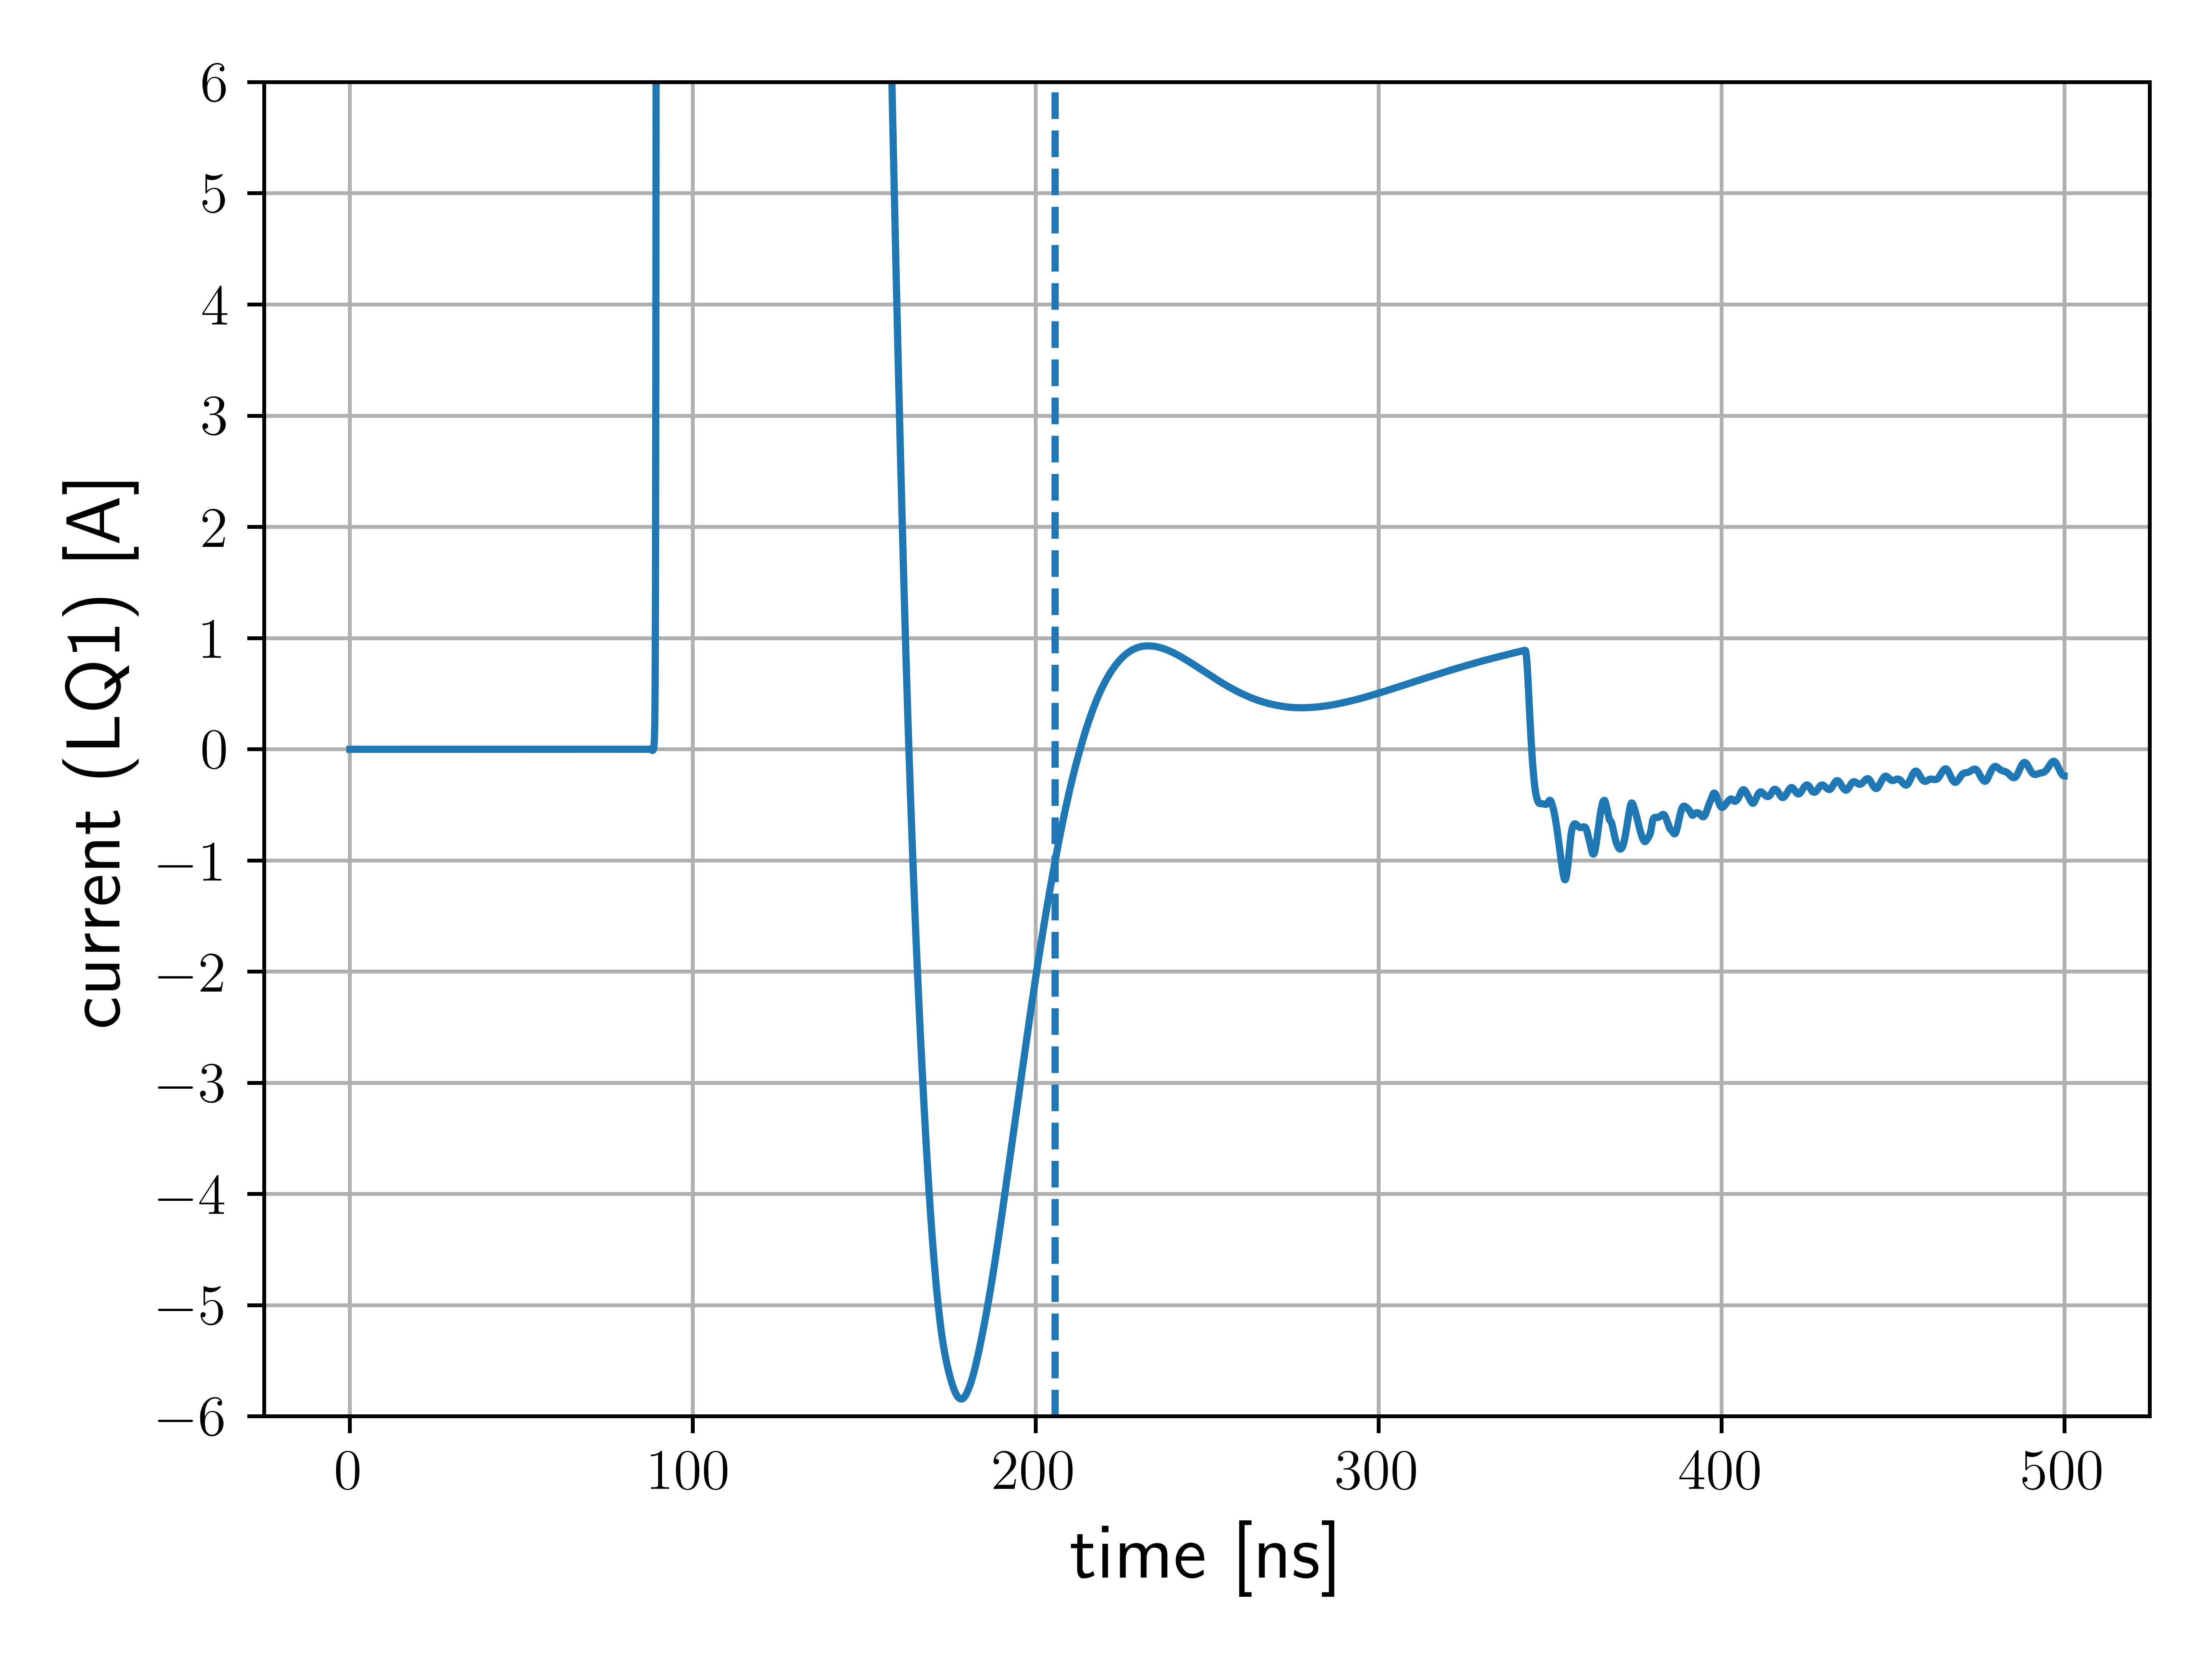
\includegraphics[width=0.3\textwidth]{Figures/muEDM/Pulser/pulse_zoom.png}}
        \hfill
        \subfloat[Charging voltage recovery ]{
        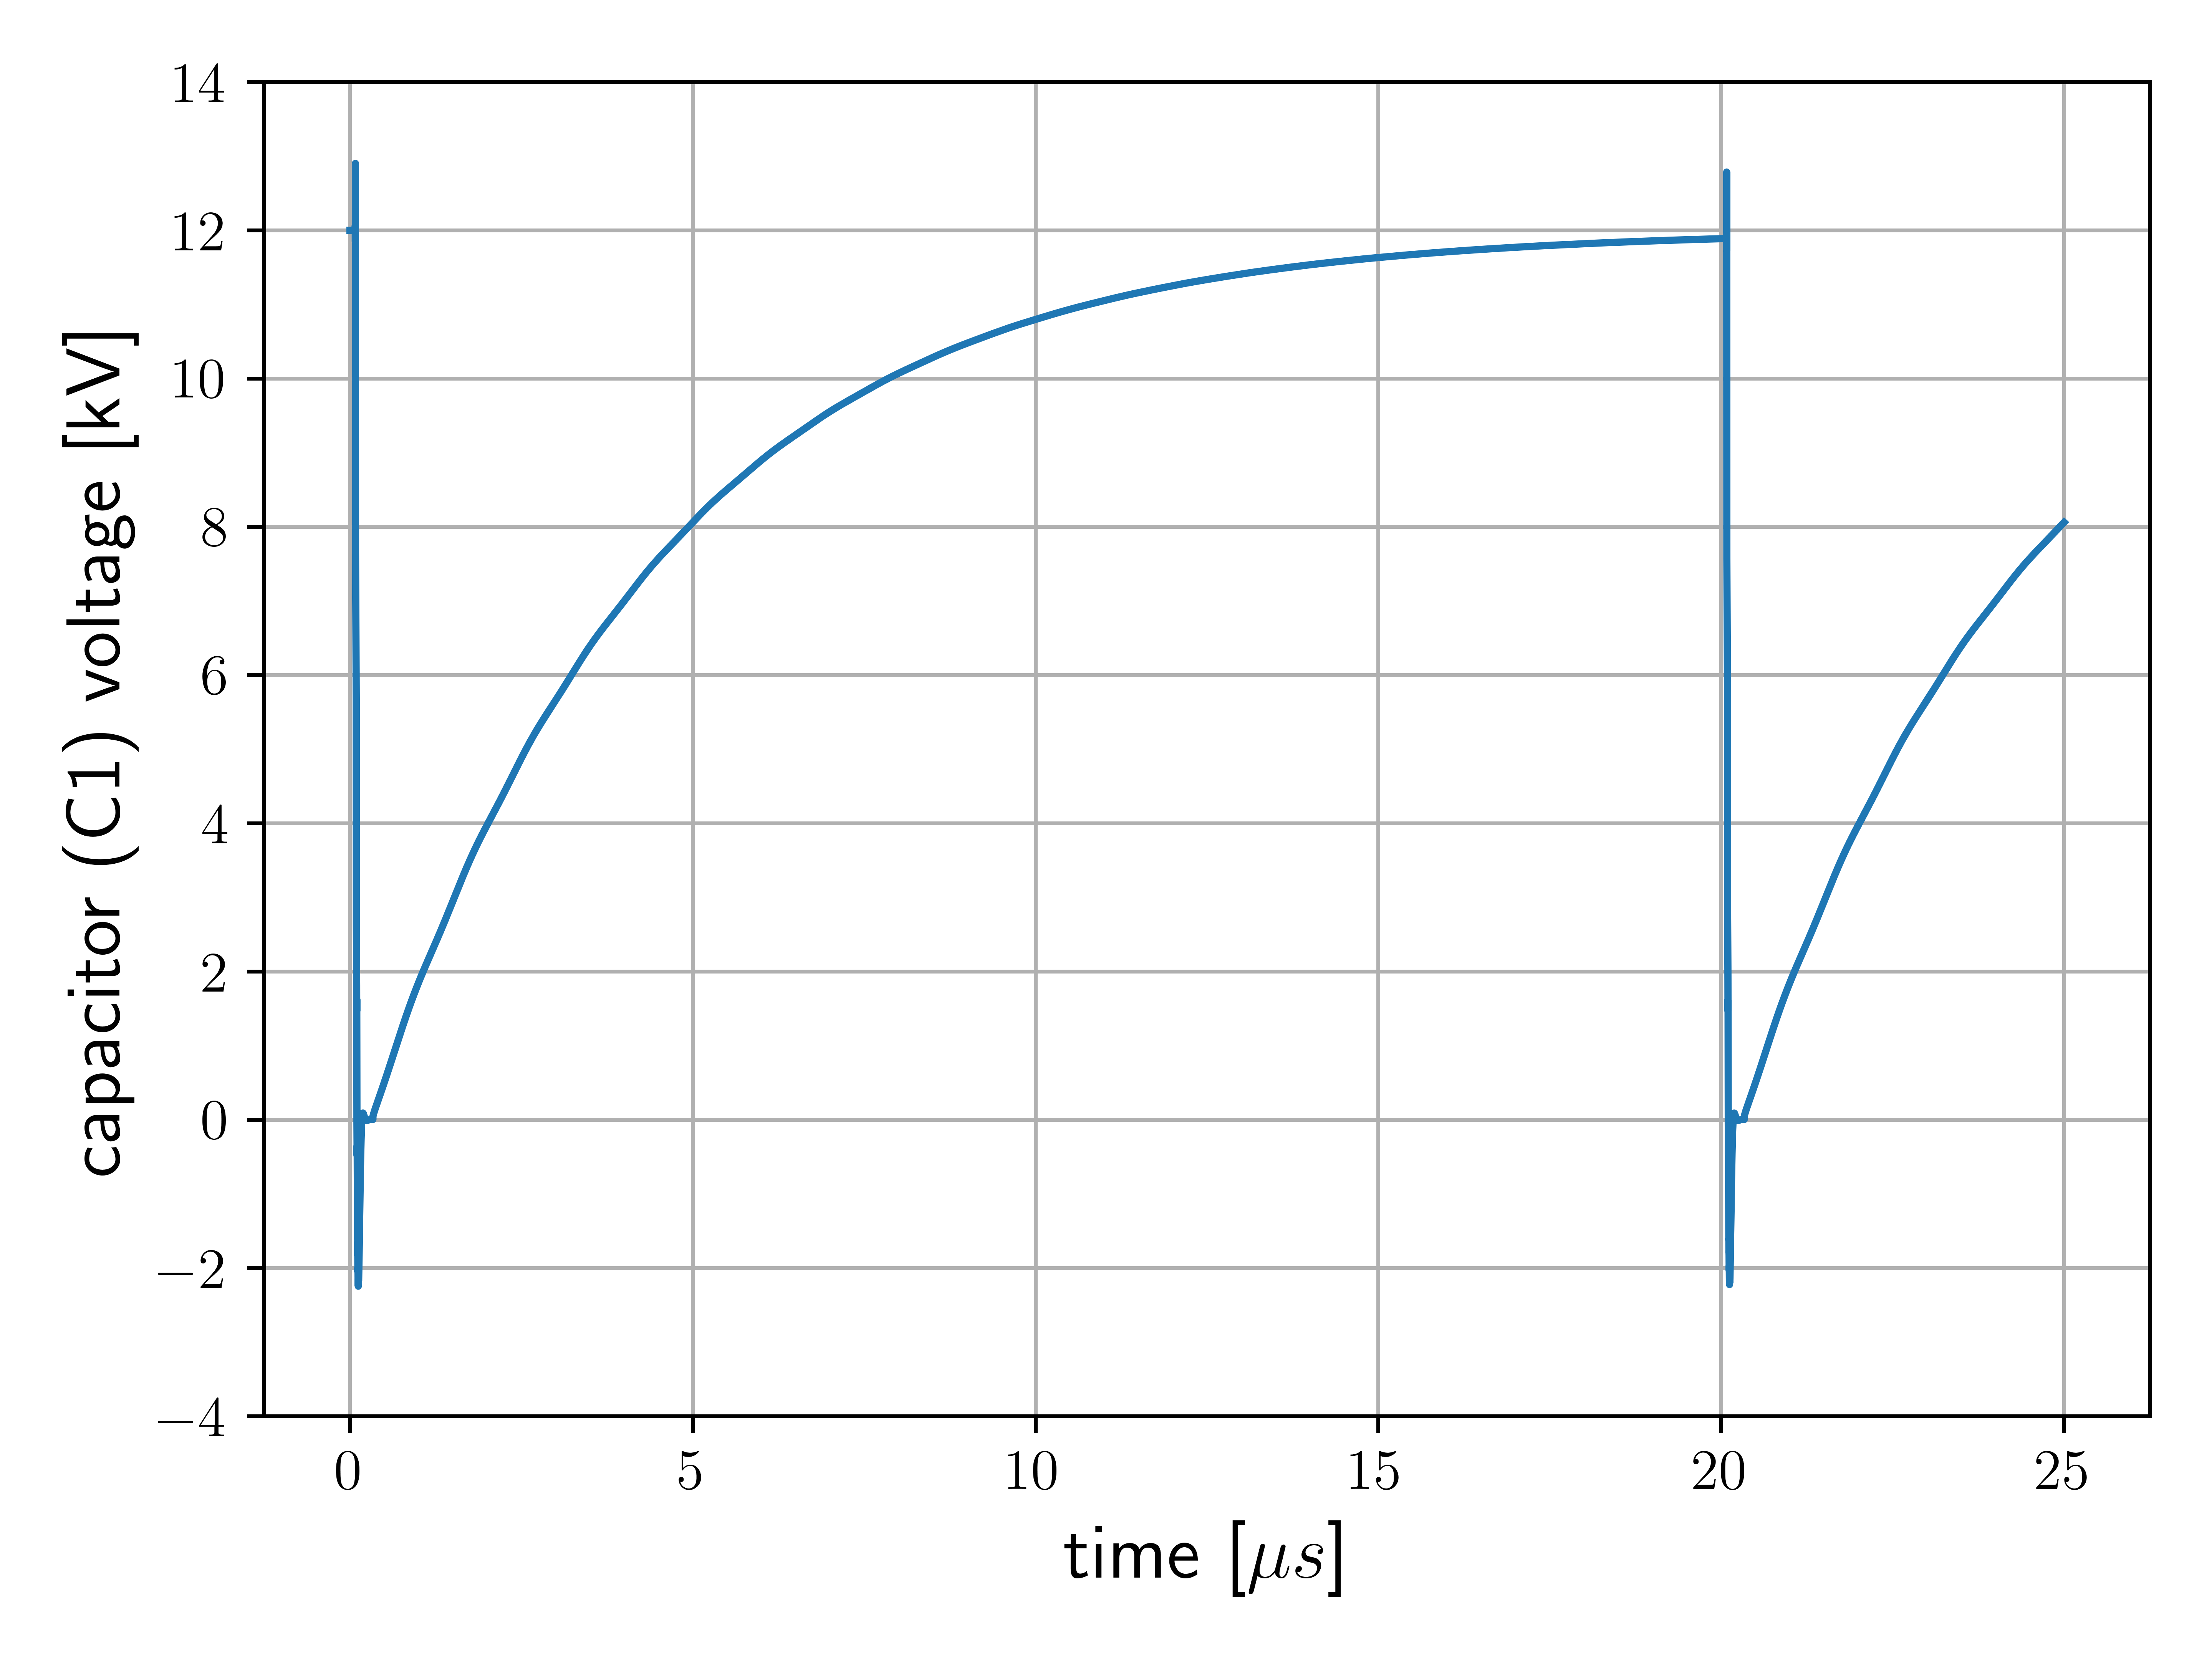
\includegraphics[width=0.3\textwidth]{Figures/muEDM/Pulser/chargingvoltage.png}}
        \caption{Pulse current profiles simulated using the LTspice circuit model with parameters as shown in Fig.~\ref{fig:circuit}. The current plotted in (a) and (b) from $t=0$ (entrance) to $t=\SI{500}{ns}$ is for the first quadrant, labeled \textit{LQ1} in Fig.~\ref{fig:circuit}. The dashed vertical line at \SI{210}{ns} indicates the time after which the current remains below $\sim 1\,A$. The voltage over the capacitor labeled \textit{C1} is plotted in (c), showing the recovery of the charging voltage within the desired \SI{20}{\micro s} duration.}
        \label{fig:pulses}
        \end{figure}

    \status{review}
    \subsection{Faraday rotator}
        To measure the field strength and time dependence of short high-intensity magnetic-field pulses, a compact sensor was designed. 
        The sensor, based on Faraday rotation\footnote{The Faraday effect causes a polarization rotation which is proportional to the projection of the magnetic field along the direction of the light propagation.}, aims for a sensitivity of a few microtesla up to 200 MHz. 
        Powered by a Toptica potassium laser, it employs a probe with a polarizer, a \SI{1}{\cm\cubed} TGG crystal with a high Verdet\footnote{The Verdet constant describes the strength of the Faraday effect in a material.} constant, a right-angle mirror, and an analyzer. 
        The laser beam passes twice through the crystal, enhancing sensitivity. 
        In Fig.~\ref{fig:faraday_probe} a picture of it.
        The angular shift in the polarization plane is measured by a ThorLabs photodiode.
        
        \noindent
        The sensor's performance was tested by applying a small AC magnetic field at \SI{100}{kHz} to the TGG crystal using a custom copper coil. 
        The setup, shown in Fig.~\ref{fig:faraday_probe}, achieved microtesla sensitivity, crucial for the \SI{100}{kHz} to \SI{10}{MHz} range. 
        The experimental results demonstrate efficient measurement of microtesla magnetic fields, enhanced by strong laser power and noise cancellation using a differential photodiode. 
        The compact design enables measurements in confined spaces, crucial for the muonEDM experimental setup.

        \begin{figure}[h]
            \centering
            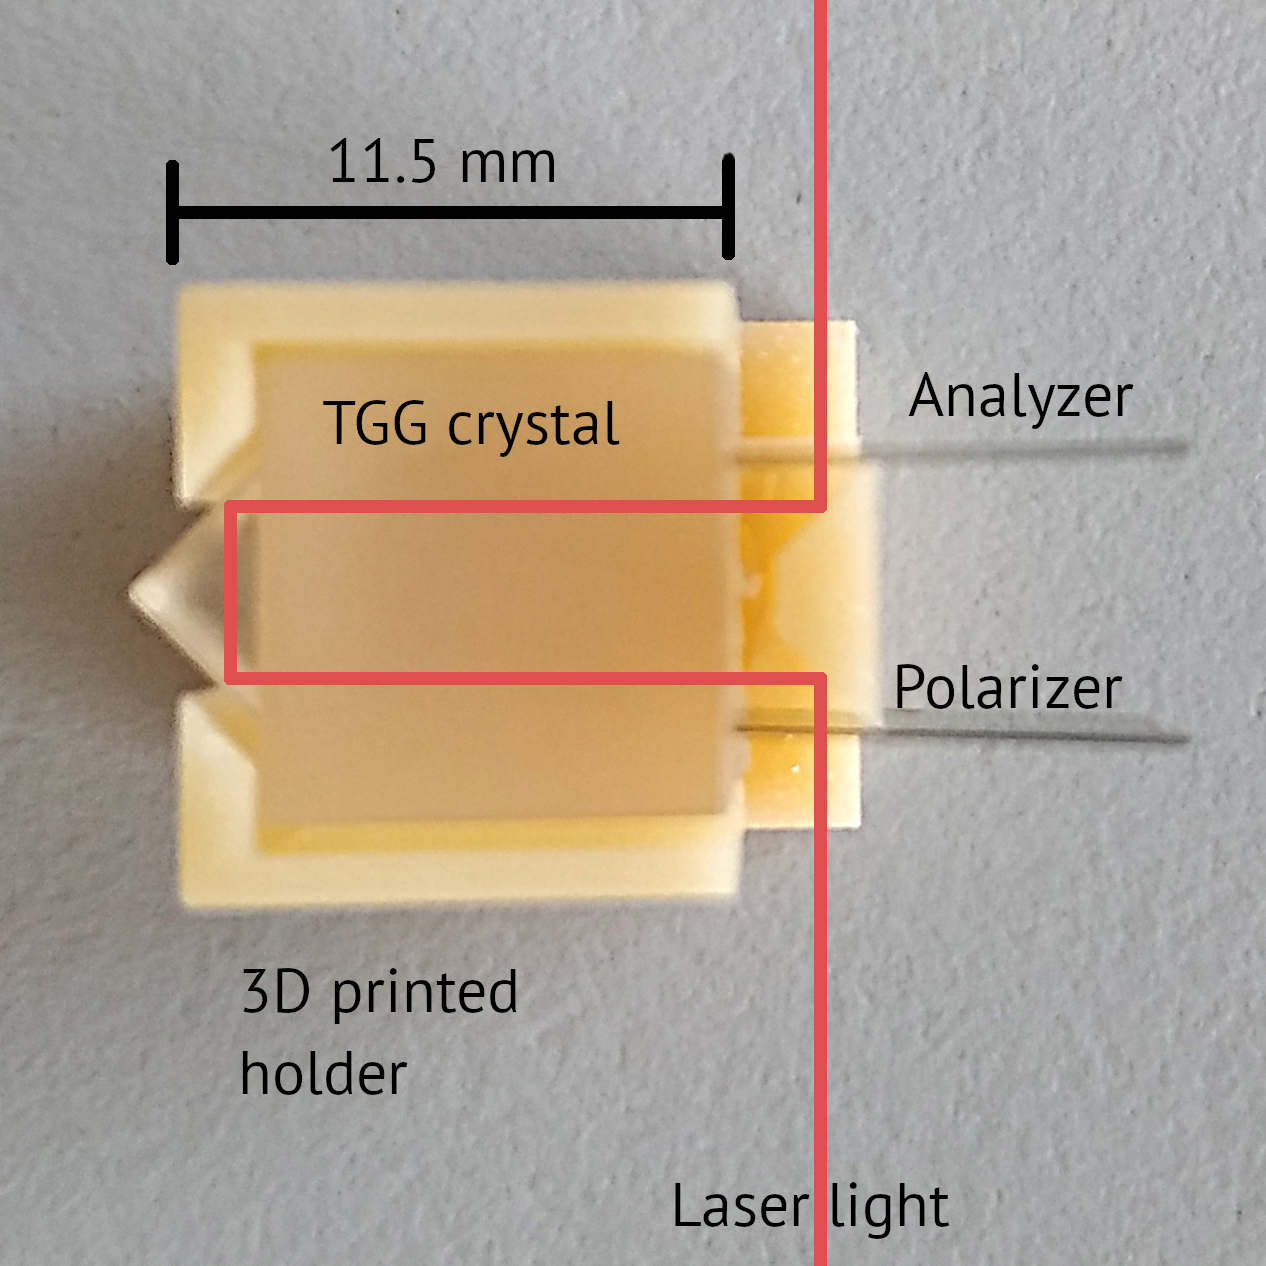
\includegraphics[height = 7cm]{Figures/muEDM/sensor.jpg}
            \hfill
            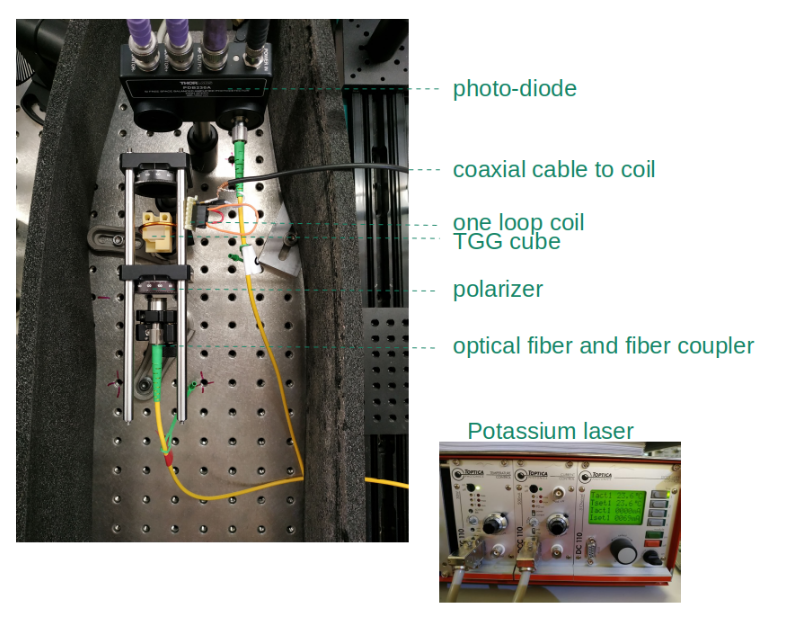
\includegraphics[height = 7cm]{Figures/muEDM/setup100kHz.png}
            \caption{Left: The TGG crystal holder with polarizer and analyzer. Center: Setup for characterization of the TGG crystal and verification of the performance of the magnetometer. The one loop coil serves to produce a micro-Tesla level field at \SI{100}{kHz}. Right: The potassium laser used to power the probe.}
        \label{fig:faraday_probe}
        \end{figure}

    \status{review}
    \subsection{Frozen-spin electrodes}
        After the muon has been successfully stored around the design orbit the next step is to apply a radial electric field. 
        The strength of this field is going to modify the frequency of the g-2 precession, eventually \textit{freezing} the spin (eq. \ref{eq:freezed}) along the momentum direction.
        The radial electric field will be induced by concentric cylindrical electrodes at $r=\SI{40}{mm}$ (grounded) and $r=\SI{20}{mm}$ (high voltage), requiring $\sim\SI{6}{kV}$ to achieve a frozen-spin field strength of $\approx\SI{3}{kV\per cm}$ at the nominal orbit radius ($\rho=\SI{31}{mm}$).
        A momentum bite of $0.5\%$ leads to a limit of approximately $1\%$ for matching the frozen-spin field strength over the momentum distribution, requiring a voltage precision better than $0.5\%$. 
        To control systematic effects from a longitudinal electric field, the applied voltage stability must be constrained to $\sim10^{-4}$.
        The 20HVA24-BP1-F high voltage amplifier by \textit{Advanced Energy}\footnote{\url{www.advancedenergy.com/en-us/products/dc-dc-conversion-products/high-voltage-boost-(u-v)/high-voltage-amplifiers/hva-series/}} meets these requirements with limited voltage ripple and a bipolar supply, enabling calibration of the frozen-spin field strength. 
        This calibration involves observing spin precession due to the anomalous magnetic moment when the electric field is offset from $E_f$. 
        The device will be tested with existing electrode prototypes to verify stability under applied high voltage in a vacuum, facilitating electric field measurements and geometric alignment. 
        This progress informs the final electrode system design for integration in 2024, with further development leading to incorporation into anticipated beam tests in 2025.

        \paragraph{Prototype}
        Prototype electrodes, made from aluminized Kapton films, were designed to study eddy currents induced by the magnetic field pulse. 
        To minimize eddy currents, material with higher resistivity or optimized geometry is crucial. 
        Measurement of the radial component at the muon orbit is necessary for shielding determination and design optimization.
        Using a \SI{5}{mm} radius pickup coil, voltages induced by a \SI{10}{\mega\hertz} sinusoidal current in the pulse coils were compared for various electrode configurations. 
        A ground electrode made from homogeneously aluminized Kapton exhibited a maximum shielding factor of $1.9(1)$, increasing to $3.0(2)$ with the HV electrode installed. 
        However, azimuthal asymmetry along the muon orbit was observed due to the discontinuity at the gluing seam.
        
        \noindent
        A new prototype with aluminum distributed in \SI{2}{mm} stripes (\SI{2.2}{mm} pitch) was prepared (see Fig.~\ref{fig:segmented}(a)). 
        Measurements with this segmented electrode showed shielding factors $<1.1$ ($90\%$ C.L.), indicating effective restriction of radial eddy-current flow across length scales comparable to the coils. 
        This allows near-complete transmission of the radial field at frequencies relevant to the magnetic field pulse, with no measurable shielding or azimuthal asymmetry.
        Noting that a segmented electrode introduces periodic field non-uniformity along the orbit, investigations were conducted to explore possible systematic effects arising from the accumulation of a geometric phase. 
        For instance, separating the electrodes into 100 longitudinal strands would induce $E$-field oscillations of approximately \SI{40}{\giga\hertz}.
        Implemented in ANSYS with 60 wires of \SI{1}{mm} diameter for the high voltage electrode and 120 for the ground (Fig.~\ref{fig:segmented}(b)), the transverse cross-section of the electric field shows negligible high-frequency oscillations for a displaced orbit (\SI{6}{mm}). The study demonstrates that a segmented electrode will not introduce additional systematic effects.
        
        \begin{figure}
            \centering
            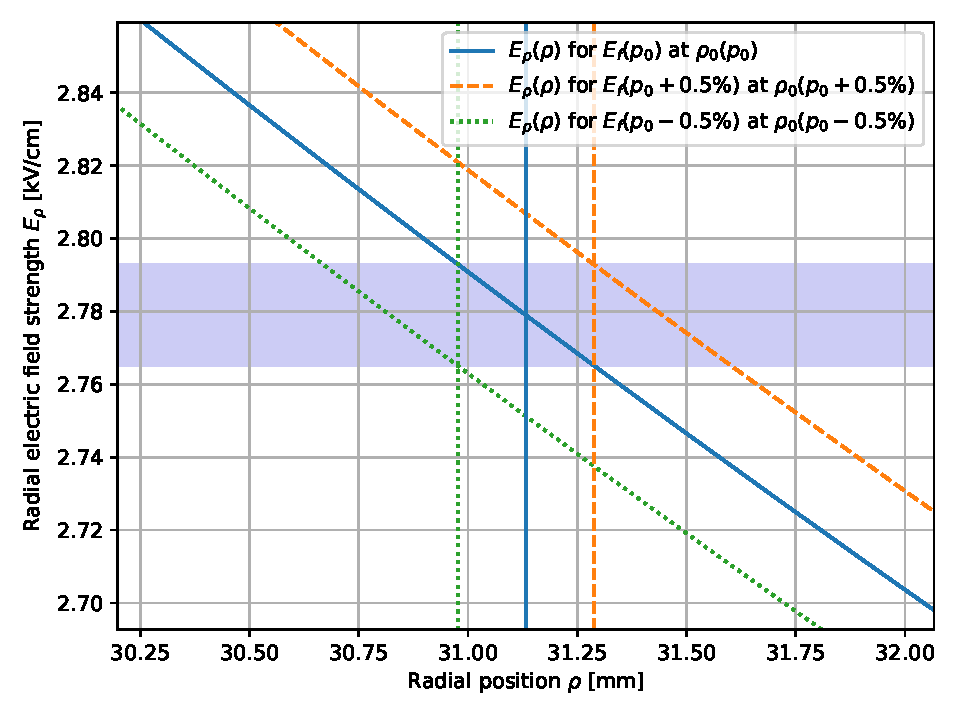
\includegraphics[width=0.8\textwidth]{Figures/muEDM/Electrode/ElectricField.pdf}
            \caption{The radial electric field corresponding to the frozen-spin field strength at the nominal orbit radius is plotted over the radial position. The dashed vertical lines indicate the radial offset due to changes in momentum $\pm0.5\%$. The dashed curves indicate the electric field which would satisfy the frozen-spin condition for these shifted momenta and radii. The resultant discrepancy is $\sim1\%$, limiting the precision necessary for the electric field strength given a momentum bite of $0.5\%$.}
            \label{fig:efieldprecision}
        \end{figure}
        
        \begin{figure}
            \centering
            \subfloat[Stripe-segmented electrode prototype]{
            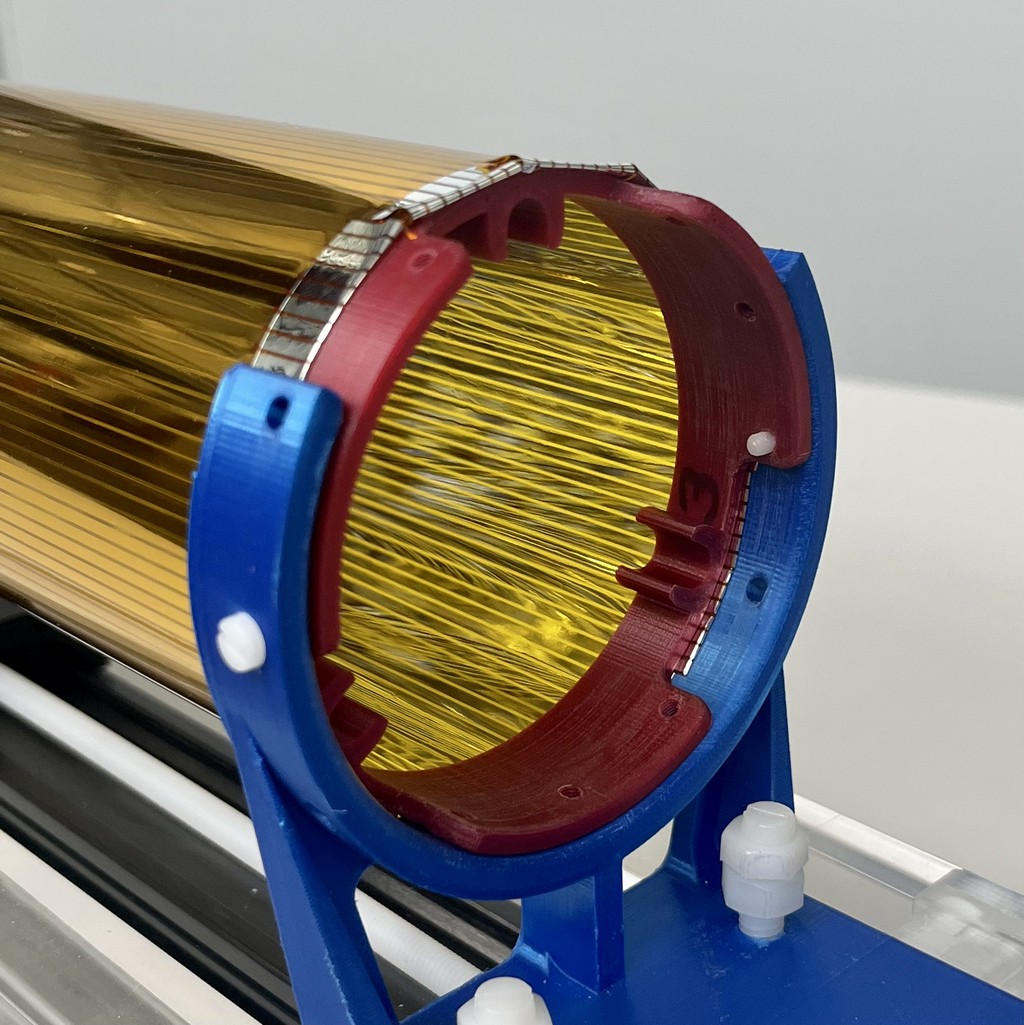
\includegraphics[height=0.4\textwidth]{Figures/muEDM/Electrode/stripedfoil.jpg}}
            \hfill
            \subfloat[Wire electrode simulation]{
            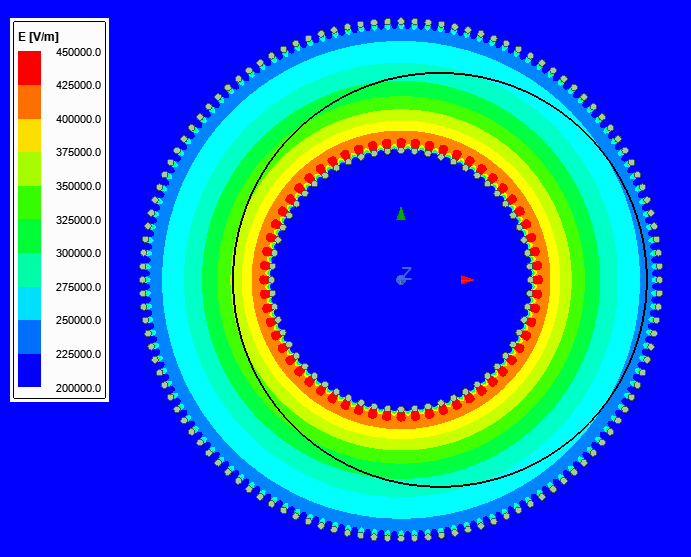
\includegraphics[height=0.4\textwidth]{Figures/muEDM/Electrode/ansys_striped_field.png}}
            \caption{A segmented electrode prevents eddy current shielding of the magnetic pulse, while preserving the required electric field properties. A prototype made from aluminized Kapton (a) showed negligible shielding, while simulation studies using a wire array electrode modeled in ANSYS (b) show no significant systematic effects and sufficient uniformity of the field in the storage region.}
        \label{fig:segmented}
        \end{figure}
    
    \status{review}
    \subsection{Positron tracking}
        The development of the positron tracker has been a big part of my work in the collaboration.
        For this reason, an in-depth description will follow in a dedicated chapter (see Ch.~\ref{ch:muEDM:tracker}) while here we will just outline the basic idea.
        The project started with a `two subsystems' approach:
        \begin{outline}
            \1 A silicon pixel external tracker will be used to track precisely the transverse position of the positron. 
            This sub-detector aims to measure the g-2 precession to fine-tune the radial electric field to achieve the frozen-spin condition.
            A straw-tube-based alternative design for this sub-detector as also been studied but later discarded.
            \1 An internal scintillating fiber detector (with comparable resolution on the transverse position) will complement the silicon pixel with additional hits. 
            The requirement is to have a better resolution on the longitudinal position of the hits to measure the EDM by looking at the pitch of the outgoing helical track.
            I dedicated most of my effort to this sub-detector.
        \end{outline}
        Unfortunately, the development of the Pixel detector met some complications and we will rely exclusively on the scintillating fibers during Phase I, prompting a review of the whole detector design.  

\status{review}
\section{Sensitivity}
\label{sec:muEDM:sensitivity}
    If the muon spin has a component parallel to the main magnetic field, the difference in probability $p$ for positron emission along ($p_\uparrow$) or opposite ($p_\downarrow$) the magnetic field will generate an asymmetry
    \begin{equation}
        A = \frac{p_\uparrow - p_\downarrow}{p_\uparrow + p_\downarrow}
    \label{eq:asym_theory}
    \end{equation}        
    For an EDM-induced spin precession, the observable is the time derivative of $A$.
    The variables $p_\uparrow$ and $p_\downarrow$ are the result of the angular distribution of Michel decay positrons
    \begin{equation}
        W(x, y)dxdy = x^2 \left((3-2x) + (2x - 1)y\right)dxdy,
    \end{equation}
    where $x = E/E_\mathrm{max}$, and $y = \lvert \vec p_\mu \cdot \vec p_e \rvert$ is the angle between the momenta of the muon and decay positron. 
    We can express the non-boosted variables in terms of the boosted ones, such as
    \begin{equation}
	u = \frac{E'}{E'_\mathrm{max}} = x\frac{\sqrt{\gamma^2 (y+\beta)^2 + 1 - y^2}}{\gamma(1+\beta)},\quad
	v = \cos\left(\arctan\frac{E'_x}{E'_z}\right) = \frac{1}{\sqrt{(E'_x/E'_z)^2 + 1}}.
    \end{equation}
    Expressing non-boosted variables with these, and with some manipulation, we obtain the boosted energy spectrum $N(u)$, the asymmetry $A(u, v)$, and its rate of change $\partial_\Psi A$ with respect to the polar angle $\Psi$ of the spin.
    For details, see \cite{chavdar:2023}.
    These variables are shown in Fig.~\ref{fig:n_dot_a} for phases I and II.
    \noindent
    The aim is then to optimize the sensitivity by applying a selection of positron energies and emission angles at the cost of statistics. Therefore, we optimize the sensitivity to $d_\mu$: $\sigma(d_\mu) \sim 1/(\alpha\sqrt{N})$ and define the figure of merit, where $N_{e^+}$ is the number of detected decay positrons, $N_{\mu^+}$ is the total number of muons stored, and $\tilde\alpha$ is the weighted average of the rate of change of the parity-violating decay asymmetry. 

    \begin{equation}
	F = \tilde\alpha \sqrt{\frac{N_{e^+}}{N_{\mu^+}}}; \ 
    \tilde\alpha = \frac{1}{N_{\mu^+}} \int \partial_\Psi A(u) N(u)
	du,
	\label{eq:figure_of_merit}
    \end{equation}

    At this point, we have a few options:
    \begin{outline}
        \1[A] The first option is to count all positrons, independently of the emission variables. This leads to $F=\tilde\alpha \approx 0.166$ for both phases I and II
        \1[T] The second option is to count only positrons above a given fractional energy $u_0$. For the two phases, maximizing the figure of merit results in 0.22 for $u_0\approx0.60$ and 0.17 for $u_0=0.18$
        \1[W] Last option is to define emission angle and/or fractional energy bins. 
        For each bin $(u, \theta, \phi)$ we can define a figure of merit $W_{ijk} = \alpha_{ijk} \sqrt{N_{ijk}}$, with $N_{ijk}$ as integral of $ N(u, \theta, \phi)$ on the $ijk$ bin, and $\alpha_{ijk}$ the integral of $ \partial_\Psi A(u,
	\theta, \phi) N(u, \theta, \phi) / N_{ijk}$.\\
        The resulting figure of merit is then $\mathcal{W} =  \sqrt{\sum_{ijk} W_{ijk}^2}$ and it's maximum is $\approx0.29$.
        On a practical level, it depends on the reconstruction in the different bins and is evaluated as:
        $$W^2_{ijk} = \frac{(N_\uparrow - N_\downarrow)^2}{N_\uparrow + N_\downarrow},\text{ and }  \dot A_{ijk} = \frac{d}{dt} \left( \frac{N_\uparrow - N_\downarrow}{N_\uparrow + N_\downarrow} \right)$$
    \end{outline}
    All these values are illustrated in Tab.~\ref{tab:AnalysisMethods}. 
    The key aspects are clearly shown in Fig.~\ref{fig:n_dot_a} and here summarized.
    In Phase I, the impact of positrons with energy below \SI{27.6}{MeV} on measurement asymmetry is negligible. 
    Optimal sensitivity is achieved when considering positrons within an opening angle range of \SI{30}{\degree} to \SI{90}{\degree}, provided their energy exceeds \SI{41}{MeV}. 
    For Phase II, valuable asymmetry information is present in emission angles up to \SI{135}{\degree} and energies surpassing \SI{21}{MeV}.
    
\begin{figure}
	\subfloat[Phase~I, $p = \SI{28}{MeV/c}$]{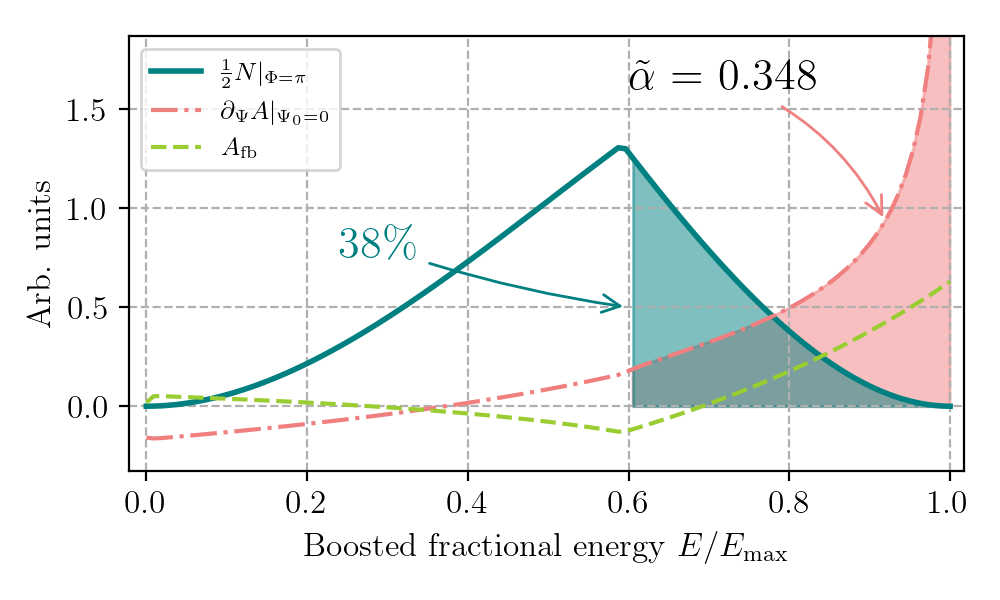
\includegraphics[width=0.49\columnwidth]{Figures/muEDM/Tracker/n_a_afb.png}}
	\hfill
	\subfloat[Phase~II, $p = \SI{125}{MeV/c}$]{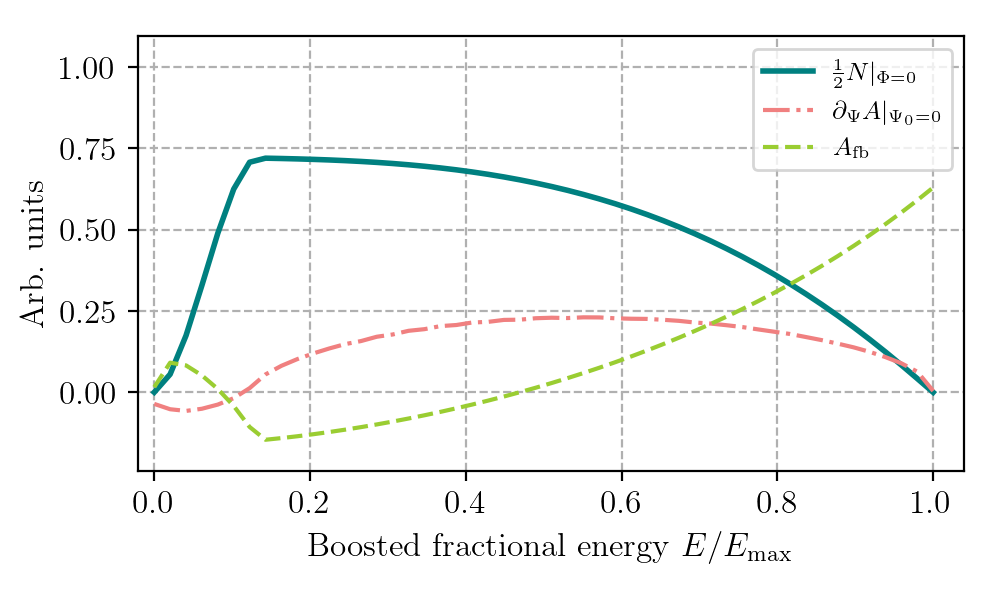
\includegraphics[width=0.49\columnwidth]{Figures/muEDM/Tracker/n_a_afb_PhaseII.png}}
	\caption{Positron energy distribution $N$, rate of change of asymmetry $\partial_\Psi A$ evaluated for spin pointing opposite and along the momentum, respectively for Phase~I and II\@. The g-2 precession is deduced from the asymmetry~($A_\mathrm{fb}$ green) between the energy distributions, while the EDM signal is proportional to the directional asymmetry~(red). The spectrum is divided into two to improve the visibility of the plot. The arrows point to the mean rate of change of asymmetry $\tilde \alpha$ and the fraction of the positron spectrum at the optimal threshold using the T-method. }
	\label{fig:n_dot_a}
\end{figure}


\begin{table}[ht]
    \begin{tabular}{@{}p{2.2cm}p{2cm}ccc@{\hspace{10pt}}p{2cm}ccc@{}}
    \toprule
    \multicolumn{1}{c}{\multirow{2}{*}{Method}} & \multicolumn{4}{c}{Phase I} & \multicolumn{4}{c}{Phase II} \\ \cmidrule(l{2pt}r{10pt}){2-5} \cmidrule(l{2pt}r{2pt}){6-9} 
    \multicolumn{1}{c}{} & Threshold \scriptsize$\times \SI{68.9}{MeV}$ & \multicolumn{1}{c}{$\tilde \alpha$} & \multicolumn{1}{c}{$N_{e^+}/N_{\mu^+}$} & \multicolumn{1}{l}{FoM} & Threshold \scriptsize$\times \SI{140.2}{MeV}$ & \multicolumn{1}{c}{$\tilde \alpha$} & \multicolumn{1}{c}{$N_{e^+}/N_{\mu^+}$} & \multicolumn{1}{c}{FoM} \\ \midrule
    Simple & None & 0.166 & 1.0 & 0.166 & None & 0.166 & 1.0 & 0.166 \\ \midrule
    T-method & 0.596 & 0.348 & 0.384 & 0.216 & 0.183 & 0.195 & 0.835 & 0.178 \\ \midrule
    W-method \scriptsize(20 energy bins) & None & 0.251 & 1.0 & 0.251 & None & 0.183 & 1.0 & 0.183 \\
    W-method \scriptsize (20 energy bins) & 0.4 & 0.280 & 0.800 & 0.250 & 0.15 & 0.194 & 0.876 & 0.183 \\ \midrule
    W-method \scriptsize (20x20x20 bins) & None & 0.292 & 1.0 & 0.292 & None & 0.280 & 1.0 & 0.280 \\
    W-method \scriptsize (20x20x20 bins) & 0.4 & 0.326 & 0.800 & 0.291 & 0.15 & 0.299 & 0.876 & 0.280 \\ \bottomrule
    \end{tabular}
    \caption[Analysis method for the muEDM search]{Summary of analysis methods. The ratio $N_{e^+}/N_{\mu^+}$ is the fraction of detected positrons with respect to the total number of injected muons and $\tilde \alpha$ is the mean asymmetry above a threshold. The presented values are the theoretical maximum and do not include the effects of multiple scattering of positrons or limited detector acceptance.}\label{tab:AnalysisMethods}
\end{table}
    
\status{review}
\section{Systematics}
\label{sec:muEDM:systematics}
    Like for the majority of the experiment at the edge of our current understanding, the systematic effects play a key role.
    Most of the studies on this topic were performed by Chavdar Dustov, Post Doc at PSI. 
    The key aspects have been compiled in a recent publication \cite{chavdar:2023}, on which this section relies. 
    For the precursor and final experiment, the expected angular velocity of the spin induced by the EDM is here evaluated. These values give us a benchmark for the systematic effects.
    \begin{equation*}
        \dot{\Pi} = 
        \begin{cases}
            \SI{21.15}{\micro rad \per \micro s};&\text{for $\beta=0.26$ and $d_\upmu=\SI{3e-21}{e cm}$} \\
            \SI{1.26}{\micro rad \per \micro s};&\text{for $\beta=0.77$ and $d_\upmu=\SI{6e-23}{e cm}$}
        \end{cases}
    \end{equation*}
    

    \status{review}
    \subsection{Possible sources of spin precessions}
    We will now outline different sources of possible spin precession. 
    From each of these sources, a limit on a specific aspect of the experiment was extracted. 
    
        \paragraph{Radial} If the particle stays at a constant radius, the coupling of the MDM with the radial component of the weakly focusing field generates a precession.
        A similar effect arises from the non-zero longitudinal electric field. This component, seen from the muon reference frame, corresponds to a radial magnetic field and also leads to a radial precession.

        \paragraph{Azimuthal} When stored in the equilibrium orbit the muons oscillate. Because of this oscillation, the momentum is not perfectly perpendicular to the longitudinal magnetic field. 
        This produces a non-zero projection of the magnetic field along the trajectory.
        On top of this, if the radial electric field is not \textit{exactly} set to the value required to freeze the spin, it will interact with the longitudinal momentum of the particle.
        
        \paragraph{$\bm{E}$ imperfections} Another source of precession can be the change of the electric field along the orbit.
        This can be the case if the axes of the magnetic field and electric fields are displaced or at an angle.
        The effect of such imperfections can be mitigated by developing two injection channels and inverting the $B$ field, obtaining `specular' trajectories (CW and CCW).
        Just like for the other sources, we will omit the calculations, which can be found in the reference \cite{chavdar:2023}. 
        In these effects, is important to consider the cylindrical symmetry of the problem and evaluate the effects averaged over the circular orbit.
        In the next order, the deviations from circular to distorted orbits are also an interesting exercise, although the approximation holds quite well.

        \paragraph{Apparent spin precession} As already discussed, a longitudinal component of the spin produces an asymmetry. 
        This asymmetry changes in time because of the coupling of the spin with the EM fields. 
        What is measured is this rate of change of the asymmetry.
        The number of observed particles in a direction will be $N_\uparrow = \Omega_\uparrow\varepsilon_\uparrow p_\uparrow N_{\mu^+} =  \kappa_\uparrow p_\uparrow N_{\mu^+}$, where $\kappa$ takes into account the acceptance and efficiency of the detector, while $p$ is the probability and $N_{\mu^+}$ the number of stopped muons.
        \begin{equation}
            A_m = \frac{1}{N_{\mu^+}} \left( \frac{n_\uparrow}{\kappa_\uparrow} - \frac{n_\downarrow}{\kappa_\downarrow} \right)
        \end{equation}
        This equation highlights why a requirement on the temporal stability of the detectors is necessary to avoid detecting apparent asymmetry.

    \status{review}
    \subsection{Comparison with \gf}
        The analytical part of this study has two types of parameters: 8 stochastic, defining the initial condition of every stored particle, and 10 constant/slowly changing parameters of the experimental setup. 
        To verify the results of the analytical mode, a \gf simulation was developed.
        In this simulation, the EM fields can be calculated or interpolated from ANSYS field maps.
        The simulation tracks the spin orientation in the muon and in the laboratory reference frame, which can be then compared with the analytic results.
        The example in Fig.~\ref{fig:muEDM:systematics} shows very good agreement.

        \begin{figure}
            \centering
            \subfloat[Comparison between the spin precession analytical description and the \gf  tracking.]{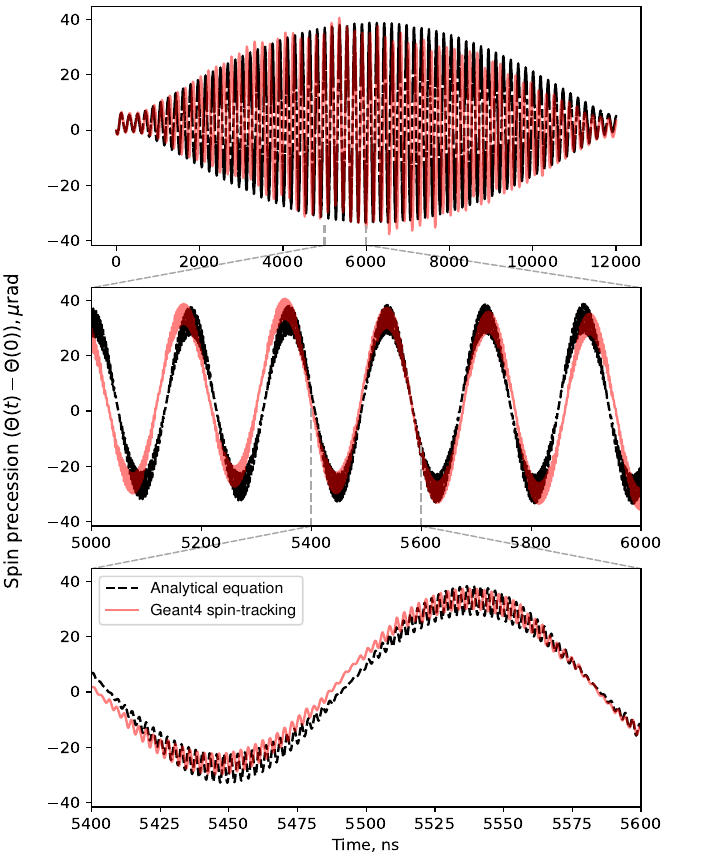
\includegraphics[height = 8.5cm]{Figures/muEDM/gf_systematics.png}}
            \hfill
            \subfloat[Constraints to avoid asymmetry rising from the electric fields. The vertical lines refer to the two Phases I and II.]{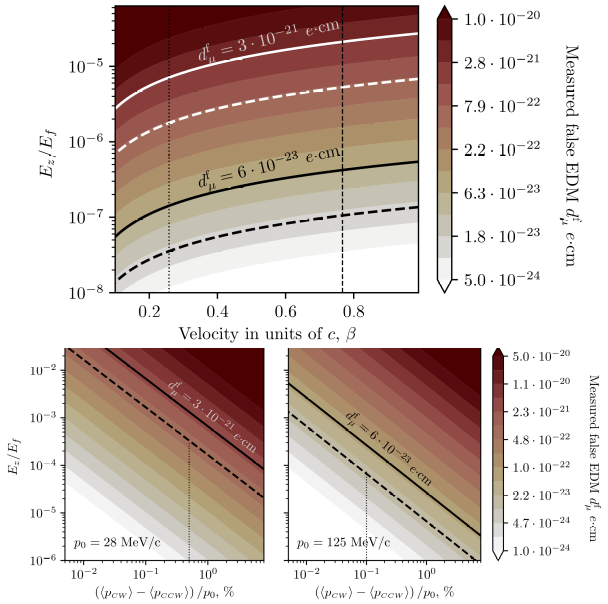
\includegraphics[height = 8.5cm]{Figures/muEDM/systemtacti_constraints.png}}
            \caption{The study on systematics has two main parts:  (a) developing and crosschecking the results extracted analytically and (b) extracting limits on the relevant parameters.}
            \label{fig:muEDM:systematics}
        \end{figure}

    \status{review}
    \subsection{Constraits} 
        To extract from each aspect a constraint on the variables at play in the experiment is not an easy task.
        Although we highlighted some key sources of real/apparent spin precession, we will not delve into the evaluation of the actual constraints and the way they can be extracted, which is partially described in \cite{chavdar:2023}.
        An example of the plot showing this type of study is in Fig.~\ref{fig:muEDM:systematics}, in which the measured `false' EDM is shown as a function of the longitudinal E field and $\beta$ of the muons.
        The introduction of the CW and CCW injection brings us to the plot in Fig.~\ref{fig:muEDM:omz_ez_limit}.
        The summary of the current understanding of the systematics is shown in Tab.~\ref{tab:SystematicEffects}.
        Fo each entry of this table plots similar to Fig.~\ref{fig:muEDM:systematics} or Fig.~\ref{fig:muEDM:omz_ez_limit} have been used, but we will not include them.
        For the detail see \cite{chavdar:2023}.

        \begin{figure}
            \centering
            \subfloat[]{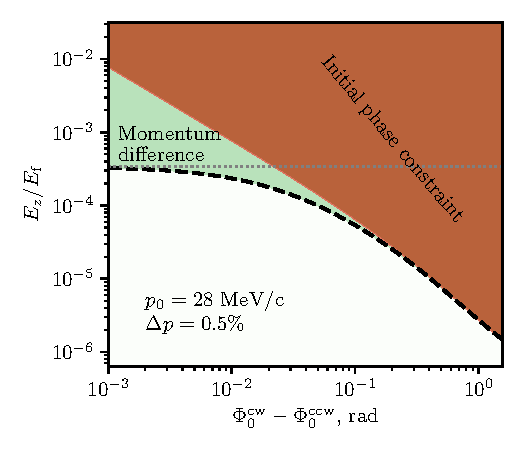
\includegraphics[width=0.526\linewidth]{Figures/muEDM/omz_ez_limit.pdf}\label{fig:omz_ez_limit_a}}
            \hfill
            \subfloat[]{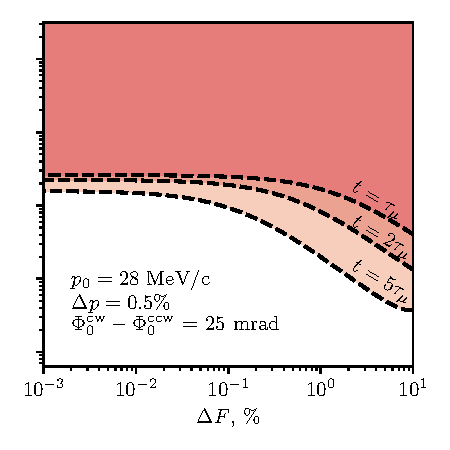
\includegraphics[width=0.451\linewidth]{Figures/muEDM/omz_speed.pdf}\label{fig:omz_ez_limit_b}}
            \caption{ Limit on the longitudinal $E$-field, $E_z$, when considering alternating CW/CCW injections, where the difference in mean momentum averaged over all injected muons for injections of CW and CCW beams is fixed at $\Delta p = 0.5\%$. 
            a)~Shows the limit as a function of the initial phase difference$\Phi_0^\mathrm{cw} - \Phi_0^\mathrm{ccw}$. 
            The horizontal dashed line indicates the limit coming from $\Delta$, keeping all other parameters equal between the two injection modes. 
            The brown area is the constraint that results from the difference in the initial phase at $\Delta p = 0\%$. 
            The green area and its thick dashed line edge show the combined limits of the two effects. 
            b)~Shows the limit as a function of the difference in $E$- or $B$-field for CW and CCW orbits, at various times. $\Delta F = 2 (F^\mathrm{cw} - F^\mathrm{ccw})/(F^\mathrm{cw} + F^\mathrm{ccw})$, where $F \in \{B_z, \tilde E_\rho \}$, while the difference in initial phases was fixed at \SI{25}{mrad}.
            }
        \label{fig:muEDM:omz_ez_limit}
        \end{figure}

        \begin{table}
            \centering
            \scriptsize
            {\renewcommand{\arraystretch}{1.2} %<- table feels too clumped without
                \begin{tabular}{@{}llcccc@{}}
                    \toprule
                    \multicolumn{1}{l}{\multirow{2}{*}{\textbf{Systematic effect}}} & \multicolumn{1}{l}{\multirow{2}{*}{\textbf{Constraints}}} & \multicolumn{2}{c}{\textbf{Phase I}} & \multicolumn{2}{c}{\textbf{Phase II}} \\ \cmidrule(l){3-6}
                    \multicolumn{1}{c}{} & \multicolumn{1}{c}{} & \multicolumn{1}{c}{\textbf{\begin{tabular}[c]{@{}c@{}}Expected\\ value\end{tabular}}} & \multicolumn{1}{c}{\textbf{\begin{tabular}[c]{@{}c@{}}Syst.\\ \scriptsize(\boldmath$\times 10^{-21} e\cdot$cm)\end{tabular}}} & \multicolumn{1}{c}{\textbf{\begin{tabular}[c]{@{}c@{}}Expected\\ value\end{tabular}}} & \multicolumn{1}{c}{\textbf{\begin{tabular}[c]{@{}c@{}}Syst.\\ \scriptsize(\boldmath$\times 10^{-23} e\cdot$cm)\end{tabular}}} \\ \midrule
                    \begin{tabular}[c]{@{}l@{}}Cone shaped electrodes\\ (longitudinal E-field)\end{tabular} & \begin{tabular}[c]{@{}l@{}}Up-down asymmetry\\ in the electrode shape\end{tabular} & $\Delta_R < 30$ \textmu m & 0.75 & $\Delta_R < 7$ \textmu m & 1.5 \\ \midrule
                    \begin{tabular}[c]{@{}l@{}}Electrode local smoothness\\ (longitudinal E-field)\end{tabular} & \begin{tabular}[c]{@{}l@{}}Local longitudinal\\ electrode smoothness\end{tabular} & $\delta_R < 3$ \textmu m & 0.75 & $\delta_R < 0.7$ \textmu m & 1.5 \\ \midrule
                    Residual B-field from kick & \begin{tabular}[c]{@{}l@{}}Decay time of\\ kicker field\end{tabular} & < 50 ns & $< 10^{-2}$ & < 50 ns & 0.5 \\ \midrule
                    \begin{tabular}[c]{@{}l@{}}Net current flowing\\ muon orbit area\end{tabular} & \begin{tabular}[c]{@{}l@{}}Wiring of electronics\\ inside the orbit\end{tabular} & < 10 mA & $< 10^{-2}$ & < 10 mA & 0.3 \\ \midrule
                    \begin{tabular}[c]{@{}l@{}}Early-to-late detection\\ efficiency change\end{tabular} & \begin{tabular}[c]{@{}l@{}}Shielding and cooling\\ of detectors\end{tabular} & -- & & -- & \\ \midrule
                    \begin{tabular}[c]{@{}l@{}}Resonant geometrical\\ phase accumulation\end{tabular} & \begin{tabular}[c]{@{}l@{}}Misalignment of\\ central axes\end{tabular} & \begin{tabular}[c]{@{}l@{}}Pitch < 1 mrad\\ Offset < 2 mm\end{tabular} & $2\times 10^{-2}$ & \begin{tabular}[c]{@{}l@{}}Pitch < 1 mrad\\ Offset < 2 mm\end{tabular} & 0.15 \\ \midrule
                    TOTAL & & & 1.1 & & 2.2 \\ \bottomrule
                \end{tabular}
            }
            \caption[Systematic effects for the muEDM search]{Summary of systematic effects for both phases of the experiment. The determination of the effects related to early-to-late detection efficiency changes is currently under evaluation.}
            \label{tab:SystematicEffects}
        \end{table}


\status{review}
\section{Schedule}
    As we just saw, although the development of the precursor is moving at a very nice speed, the tasks are very challenging.
    To put in perspective the current understanding of the different challenges and time constraints, we add here the schedule that was included in the proposal of the experiment in 2022.
    Fig.~\ref{fig:muEDM:schedule:short} is a schedule on the short period up to the long shut-down, in which 6 main milestones are highlighted:
    \begin{outline}
        \1[1] Demonstration of off-axis injection
        \1[2] Muon selection and generation of trigger
        \1[3] Generation of the pulsed magnetic field and measurement of eddy-currents
        \1[4] Stopping of muons and detection of $(g - 2)$ precession
        \1[5] Adjusting the electric field by tuning $(g - 2)$ precession to zero
        \1[6] Data-taking in muon EDM mode
    \end{outline}
    Fig.~\ref{fig:muEDM:schedule:long} goes beyond the long shut-down and covers the full life of the experiment, up to 2033.
    
    \begin{figure}
        \centering
        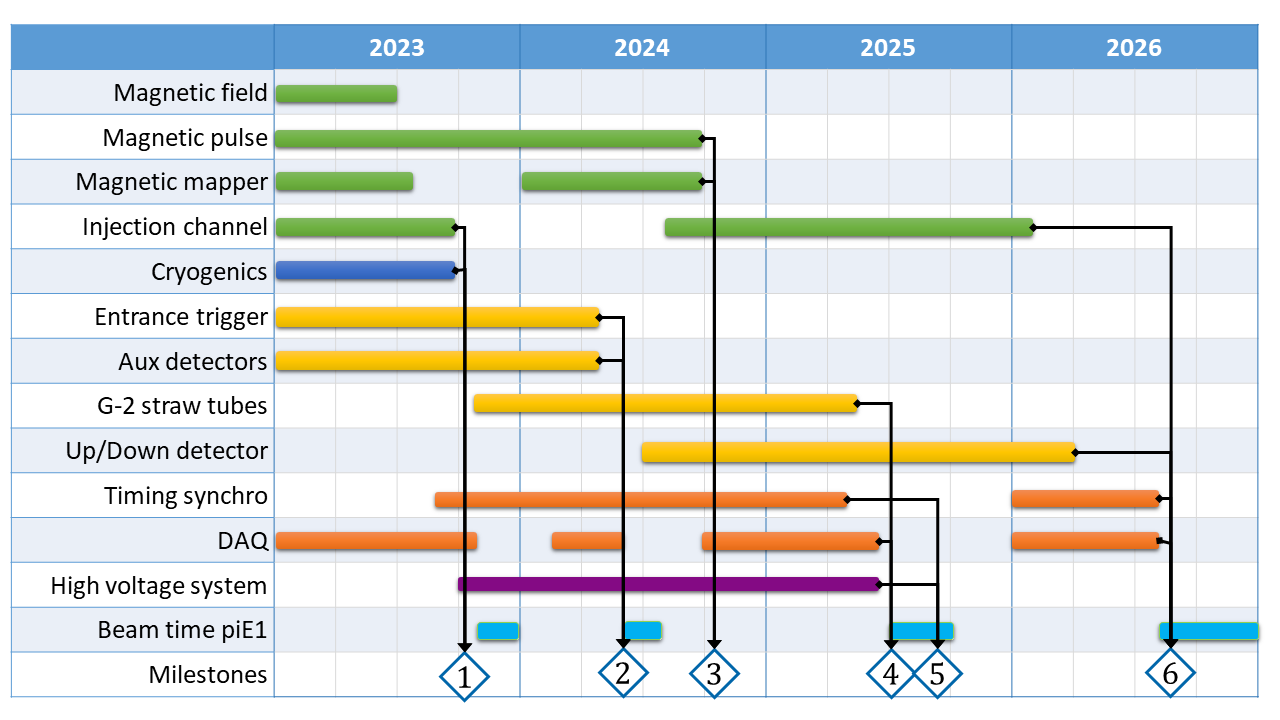
\includegraphics[width = \textwidth]{Figures/muEDM/Schedule2023-2026.png}
        \caption{`Short' term muEDM schedule, with highlighted the 6 main milestones up to the \textit{long shutdown}. Milestones: 1) off-axis injection; 2) generation of the entrance trigger; 3) generation of the pulsed B field; 4) detection of $g-2$; 5) adjust $g-2$ to zero; 6) EDM data taking.}
        \label{fig:muEDM:schedule:short}
    \end{figure}
       
    \begin{figure}
        \centering
        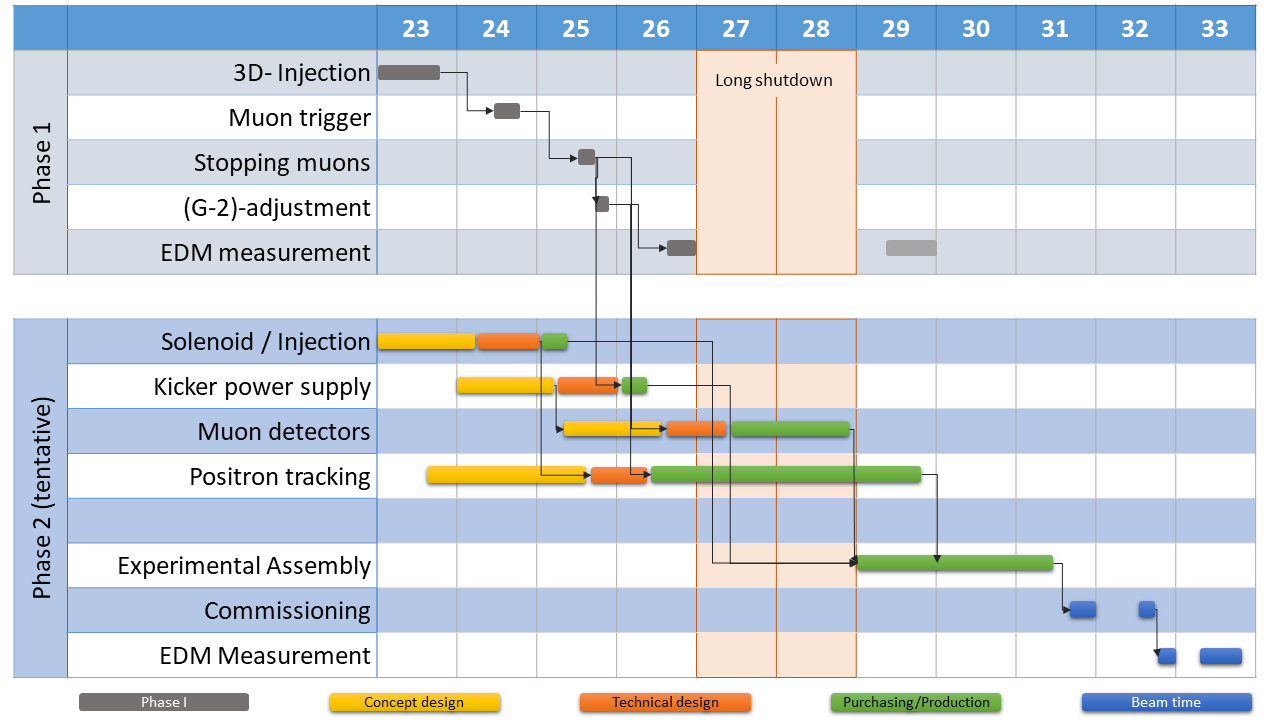
\includegraphics[width = \textwidth]{Figures/muEDM/SchedPropLongTerm23.png}
        \caption{`Long' term muEDM schedule, with the different phases up to the end of the experiment.}
        \label{fig:muEDM:schedule:long}
    \end{figure}

\status{review}
\section{Conclusions}
    After reviewing the concept of EDM, the current limits, and the frozen spin technique, we described the MuEDM experiment.
    A description of the different subsistem and their current status was given, leaving the muon detection and the positron tracking for the Ch.~\ref{ch:muEDM:entrance} and Ch.~\ref{ch:muEDM:tracker}.
    A status on the study of the systematics and a brief section on the upcoming schedule end the chapter.
    The experiment is still in an early phase but a lot of progress has been made during the last 2/3 years.
\status{started}
\printbibliography[
    heading = bibliographychapter,
    title=Bibliography on muEDM
]

\end{refsection}
